\documentclass[]{book}
\usepackage{lmodern}
\usepackage{amssymb,amsmath}
\usepackage{ifxetex,ifluatex}
\usepackage{fixltx2e} % provides \textsubscript
\ifnum 0\ifxetex 1\fi\ifluatex 1\fi=0 % if pdftex
  \usepackage[T1]{fontenc}
  \usepackage[utf8]{inputenc}
\else % if luatex or xelatex
  \ifxetex
    \usepackage{mathspec}
  \else
    \usepackage{fontspec}
  \fi
  \defaultfontfeatures{Ligatures=TeX,Scale=MatchLowercase}
\fi
% use upquote if available, for straight quotes in verbatim environments
\IfFileExists{upquote.sty}{\usepackage{upquote}}{}
% use microtype if available
\IfFileExists{microtype.sty}{%
\usepackage{microtype}
\UseMicrotypeSet[protrusion]{basicmath} % disable protrusion for tt fonts
}{}
\usepackage[margin=1in]{geometry}
\usepackage{hyperref}
\hypersetup{unicode=true,
            pdftitle={Machine Learning with the MicrosoftML Package},
            pdfauthor={Ali Zaidi},
            pdfborder={0 0 0},
            breaklinks=true}
\urlstyle{same}  % don't use monospace font for urls
\usepackage{natbib}
\bibliographystyle{apalike}
\usepackage{color}
\usepackage{fancyvrb}
\newcommand{\VerbBar}{|}
\newcommand{\VERB}{\Verb[commandchars=\\\{\}]}
\DefineVerbatimEnvironment{Highlighting}{Verbatim}{commandchars=\\\{\}}
% Add ',fontsize=\small' for more characters per line
\usepackage{framed}
\definecolor{shadecolor}{RGB}{248,248,248}
\newenvironment{Shaded}{\begin{snugshade}}{\end{snugshade}}
\newcommand{\KeywordTok}[1]{\textcolor[rgb]{0.13,0.29,0.53}{\textbf{#1}}}
\newcommand{\DataTypeTok}[1]{\textcolor[rgb]{0.13,0.29,0.53}{#1}}
\newcommand{\DecValTok}[1]{\textcolor[rgb]{0.00,0.00,0.81}{#1}}
\newcommand{\BaseNTok}[1]{\textcolor[rgb]{0.00,0.00,0.81}{#1}}
\newcommand{\FloatTok}[1]{\textcolor[rgb]{0.00,0.00,0.81}{#1}}
\newcommand{\ConstantTok}[1]{\textcolor[rgb]{0.00,0.00,0.00}{#1}}
\newcommand{\CharTok}[1]{\textcolor[rgb]{0.31,0.60,0.02}{#1}}
\newcommand{\SpecialCharTok}[1]{\textcolor[rgb]{0.00,0.00,0.00}{#1}}
\newcommand{\StringTok}[1]{\textcolor[rgb]{0.31,0.60,0.02}{#1}}
\newcommand{\VerbatimStringTok}[1]{\textcolor[rgb]{0.31,0.60,0.02}{#1}}
\newcommand{\SpecialStringTok}[1]{\textcolor[rgb]{0.31,0.60,0.02}{#1}}
\newcommand{\ImportTok}[1]{#1}
\newcommand{\CommentTok}[1]{\textcolor[rgb]{0.56,0.35,0.01}{\textit{#1}}}
\newcommand{\DocumentationTok}[1]{\textcolor[rgb]{0.56,0.35,0.01}{\textbf{\textit{#1}}}}
\newcommand{\AnnotationTok}[1]{\textcolor[rgb]{0.56,0.35,0.01}{\textbf{\textit{#1}}}}
\newcommand{\CommentVarTok}[1]{\textcolor[rgb]{0.56,0.35,0.01}{\textbf{\textit{#1}}}}
\newcommand{\OtherTok}[1]{\textcolor[rgb]{0.56,0.35,0.01}{#1}}
\newcommand{\FunctionTok}[1]{\textcolor[rgb]{0.00,0.00,0.00}{#1}}
\newcommand{\VariableTok}[1]{\textcolor[rgb]{0.00,0.00,0.00}{#1}}
\newcommand{\ControlFlowTok}[1]{\textcolor[rgb]{0.13,0.29,0.53}{\textbf{#1}}}
\newcommand{\OperatorTok}[1]{\textcolor[rgb]{0.81,0.36,0.00}{\textbf{#1}}}
\newcommand{\BuiltInTok}[1]{#1}
\newcommand{\ExtensionTok}[1]{#1}
\newcommand{\PreprocessorTok}[1]{\textcolor[rgb]{0.56,0.35,0.01}{\textit{#1}}}
\newcommand{\AttributeTok}[1]{\textcolor[rgb]{0.77,0.63,0.00}{#1}}
\newcommand{\RegionMarkerTok}[1]{#1}
\newcommand{\InformationTok}[1]{\textcolor[rgb]{0.56,0.35,0.01}{\textbf{\textit{#1}}}}
\newcommand{\WarningTok}[1]{\textcolor[rgb]{0.56,0.35,0.01}{\textbf{\textit{#1}}}}
\newcommand{\AlertTok}[1]{\textcolor[rgb]{0.94,0.16,0.16}{#1}}
\newcommand{\ErrorTok}[1]{\textcolor[rgb]{0.64,0.00,0.00}{\textbf{#1}}}
\newcommand{\NormalTok}[1]{#1}
\usepackage{longtable,booktabs}
\usepackage{graphicx,grffile}
\makeatletter
\def\maxwidth{\ifdim\Gin@nat@width>\linewidth\linewidth\else\Gin@nat@width\fi}
\def\maxheight{\ifdim\Gin@nat@height>\textheight\textheight\else\Gin@nat@height\fi}
\makeatother
% Scale images if necessary, so that they will not overflow the page
% margins by default, and it is still possible to overwrite the defaults
% using explicit options in \includegraphics[width, height, ...]{}
\setkeys{Gin}{width=\maxwidth,height=\maxheight,keepaspectratio}
\IfFileExists{parskip.sty}{%
\usepackage{parskip}
}{% else
\setlength{\parindent}{0pt}
\setlength{\parskip}{6pt plus 2pt minus 1pt}
}
\setlength{\emergencystretch}{3em}  % prevent overfull lines
\providecommand{\tightlist}{%
  \setlength{\itemsep}{0pt}\setlength{\parskip}{0pt}}
\setcounter{secnumdepth}{5}
% Redefines (sub)paragraphs to behave more like sections
\ifx\paragraph\undefined\else
\let\oldparagraph\paragraph
\renewcommand{\paragraph}[1]{\oldparagraph{#1}\mbox{}}
\fi
\ifx\subparagraph\undefined\else
\let\oldsubparagraph\subparagraph
\renewcommand{\subparagraph}[1]{\oldsubparagraph{#1}\mbox{}}
\fi

%%% Use protect on footnotes to avoid problems with footnotes in titles
\let\rmarkdownfootnote\footnote%
\def\footnote{\protect\rmarkdownfootnote}

%%% Change title format to be more compact
\usepackage{titling}

% Create subtitle command for use in maketitle
\newcommand{\subtitle}[1]{
  \posttitle{
    \begin{center}\large#1\end{center}
    }
}

\setlength{\droptitle}{-2em}
  \title{Machine Learning with the \texttt{MicrosoftML} Package}
  \pretitle{\vspace{\droptitle}\centering\huge}
  \posttitle{\par}
  \author{Ali Zaidi}
  \preauthor{\centering\large\emph}
  \postauthor{\par}
  \predate{\centering\large\emph}
  \postdate{\par}
  \date{2017-09-14}

\usepackage{booktabs}
\usepackage{amsthm}
\makeatletter
\def\thm@space@setup{%
  \thm@preskip=8pt plus 2pt minus 4pt
  \thm@postskip=\thm@preskip
}
\makeatother

\usepackage{amsthm}
\newtheorem{theorem}{Theorem}[chapter]
\newtheorem{lemma}{Lemma}[chapter]
\theoremstyle{definition}
\newtheorem{definition}{Definition}[chapter]
\newtheorem{corollary}{Corollary}[chapter]
\newtheorem{proposition}{Proposition}[chapter]
\theoremstyle{definition}
\newtheorem{example}{Example}[chapter]
\theoremstyle{definition}
\newtheorem{exercise}{Exercise}[chapter]
\theoremstyle{remark}
\newtheorem*{remark}{Remark}
\newtheorem*{solution}{Solution}
\begin{document}
\maketitle

{
\setcounter{tocdepth}{1}
\tableofcontents
}
\chapter{Prerequisites}\label{prerequisites}

This workshop covers the fundamentals of statistical machine learning
with the
\href{https://msdn.microsoft.com/en-us/microsoft-r/microsoftml-introduction}{MicrosoftML
package}.

MicrosoftML is a package that works in tandem with the
\href{https://msdn.microsoft.com/en-us/microsoft-r/scaler-getting-started}{RevoScaleR}
package and Microsoft R Server. In order to use the \texttt{MicrosoftML}
and \texttt{RevoScaleR} libraries, you need an installation of Microsoft
R Server or Microsoft R Client. You can download \textbf{Microsoft R
Server} through MSDN here:

\begin{enumerate}
\def\labelenumi{\arabic{enumi}.}
\tightlist
\item
  \href{https://msdn.microsoft.com/en-us/microsoft-r/rserver-install-linux-server}{R
  Server for Linux}
\item
  \href{https://msdn.microsoft.com/en-us/microsoft-r/rserver-install-hadoop}{R
  Server for Hadoop}
\item
  \href{https://msdn.microsoft.com/en-us/microsoft-r/rserver-install-windows}{R
  Server for Windows}
\item
  \href{https://docs.microsoft.com/en-us/sql/advanced-analytics/r/set-up-sql-server-r-services-in-database}{R
  Server for SQL Server (In-Database)}
\end{enumerate}

You can download \textbf{Microsoft R Client} through the following
sources:

\begin{enumerate}
\def\labelenumi{\arabic{enumi}.}
\tightlist
\item
  \href{https://msdn.microsoft.com/en-us/microsoft-r/r-client-install-windows}{R
  Client for Windows}
\item
  \href{https://msdn.microsoft.com/en-us/microsoft-r/r-client-install-linux}{R
  Client for Linux}
\item
  \href{https://github.com/akzaidi/mrclient-docker}{R Client Docker
  Image}
\end{enumerate}

\section{MicrosoftML References}\label{microsoftml-references}

\begin{itemize}
\tightlist
\item
  \href{https://msdn.microsoft.com/en-us/microsoft-r/microsoftml-algorithm-cheat-sheet}{Cheat
  Sheet}
\item
  \href{https://msdn.microsoft.com/en-us/microsoft-r/overview-microsoftml-functions}{Overview
  of MicrosoftML Functions}
\item
  \href{https://msdn.microsoft.com/en-us/microsoft-r/microsoftml/microsoftml}{Function
  Reference}
\item
  \href{https://msdn.microsoft.com/en-us/microsoft-r/microsoftml-quickstarts}{Quickstarts}
\item
  \href{https://msdn.microsoft.com/en-us/microsoft-r/}{MSDN Site for
  Microsoft R Server}
\item
  \href{https://msdn.microsoft.com/en-us/microsoft-r/r-client}{MSDN Site
  for Microsoft R Client}

  \begin{itemize}
  \tightlist
  \item
    \href{https://channel9.msdn.com/blogs/MicrosoftR/Microsoft-Introduces-new-free-Microsoft-R-Client}{R
    Client Overview}
  \end{itemize}
\end{itemize}

\section{Useful Resources}\label{useful-resources}

\begin{itemize}
\tightlist
\item
  \href{https://lagunita.stanford.edu/courses/HumanitiesSciences/StatLearning/Winter2016/about}{Introduction
  to Statistical Learning Video Lectures}

  \begin{itemize}
  \tightlist
  \item
    My favorite course on statistical learning
  \item
    Worth doing twice!
  \end{itemize}
\item
  \href{http://www-bcf.usc.edu/~gareth/ISL/}{Introduction to Statistical
  Learning Textbook}

  \begin{itemize}
  \tightlist
  \item
    \emph{Baby Statistical Learning}
  \end{itemize}
\item
  \href{http://statweb.stanford.edu/~tibs/ElemStatLearn/}{Elements of
  Statistical Learning Textbook}

  \begin{itemize}
  \tightlist
  \item
    \textbf{Papa Statistical Learning}
  \end{itemize}
\item
  \href{http://r4ds.had.co.nz/}{R for Data Science}

  \begin{itemize}
  \tightlist
  \item
    Covers the core tools in the
    \href{http://tidyverse.org/}{\texttt{tidyverse}} ecosystem for data
    science and analytics
  \end{itemize}
\item
  \href{https://github.com/Azure/LearnAnalytics-mr4ds}{Microsoft R for
  Data Science}

  \begin{itemize}
  \tightlist
  \item
    My two-day workshop on Microsoft R Server for Data Science
  \end{itemize}
\item
  \href{https://github.com/Azure/LearnAnalytics-mrs-spark}{Microsoft R
  Server and Spark}

  \begin{itemize}
  \tightlist
  \item
    My 1.5 day course on Microsoft R Server and Spark Integration
  \end{itemize}
\item
  \href{https://bookdown.org/alizaidi/mrs-spark-ml/}{Scalable Data
  Science with Microsoft R Server and Spark}

  \begin{itemize}
  \tightlist
  \item
    In progress book on data science with Microsoft R Server and Spark
  \end{itemize}
\end{itemize}

\chapter{Exploratory Data Analysis and Feature
Engineering}\label{exploratory-data-analysis-and-feature-engineering}

Import your favorite libraries and set up your favorite plotting theme.

\begin{Shaded}
\begin{Highlighting}[]
\KeywordTok{library}\NormalTok{(tidyverse)}
\KeywordTok{theme_set}\NormalTok{(}\KeywordTok{theme_minimal}\NormalTok{())}
\end{Highlighting}
\end{Shaded}

Now let's import some data. Our
\href{http://www.dcc.fc.up.pt/~ltorgo/Regression/cal_housing.html}{data
source} is 1990-census level of housing in California.

We'll use easy the \texttt{readr} package to load in our data. You could
equivalently use \texttt{read.csv}, or \texttt{data.table::fread} if you
wanted incredible speed. We'll later see how to use data sources using
the \texttt{RevoScaleR} readers.

Since we're using \texttt{readr}, our data is a \texttt{tbl}. This means
we will get some \texttt{dplyr} and \texttt{tibble} features, and it'll
behave a little differently than a traditional \texttt{data.frame}.

\begin{Shaded}
\begin{Highlighting}[]
\NormalTok{housing <-}\StringTok{ }\KeywordTok{read_csv}\NormalTok{(}\StringTok{"data/housing.csv"}\NormalTok{)}
\KeywordTok{class}\NormalTok{(housing)}
\end{Highlighting}
\end{Shaded}

\begin{verbatim}
## [1] "tbl_df"     "tbl"        "data.frame"
\end{verbatim}

\begin{Shaded}
\begin{Highlighting}[]
\KeywordTok{glimpse}\NormalTok{(housing)}
\end{Highlighting}
\end{Shaded}

\begin{verbatim}
## Observations: 20,640
## Variables: 10
## $ longitude          <dbl> -122.23, -122.22, -122.24, -122.25, -122.25...
## $ latitude           <dbl> 37.88, 37.86, 37.85, 37.85, 37.85, 37.85, 3...
## $ housing_median_age <dbl> 41, 21, 52, 52, 52, 52, 52, 52, 42, 52, 52,...
## $ total_rooms        <dbl> 880, 7099, 1467, 1274, 1627, 919, 2535, 310...
## $ total_bedrooms     <dbl> 129, 1106, 190, 235, 280, 213, 489, 687, 66...
## $ population         <dbl> 322, 2401, 496, 558, 565, 413, 1094, 1157, ...
## $ households         <dbl> 126, 1138, 177, 219, 259, 193, 514, 647, 59...
## $ median_income      <dbl> 8.3252, 8.3014, 7.2574, 5.6431, 3.8462, 4.0...
## $ median_house_value <dbl> 452600, 358500, 352100, 341300, 342200, 269...
## $ ocean_proximity    <chr> "NEAR BAY", "NEAR BAY", "NEAR BAY", "NEAR B...
\end{verbatim}

\begin{Shaded}
\begin{Highlighting}[]
\NormalTok{housing}
\end{Highlighting}
\end{Shaded}

\begin{verbatim}
## # A tibble: 20,640 x 10
##    longitude latitude housing_median_age total_rooms total_bedrooms
##        <dbl>    <dbl>              <dbl>       <dbl>          <dbl>
##  1   -122.23    37.88                 41         880            129
##  2   -122.22    37.86                 21        7099           1106
##  3   -122.24    37.85                 52        1467            190
##  4   -122.25    37.85                 52        1274            235
##  5   -122.25    37.85                 52        1627            280
##  6   -122.25    37.85                 52         919            213
##  7   -122.25    37.84                 52        2535            489
##  8   -122.25    37.84                 52        3104            687
##  9   -122.26    37.84                 42        2555            665
## 10   -122.25    37.84                 52        3549            707
## # ... with 20,630 more rows, and 5 more variables: population <dbl>,
## #   households <dbl>, median_income <dbl>, median_house_value <dbl>,
## #   ocean_proximity <chr>
\end{verbatim}

\section{Visualize Densities}\label{visualize-densities}

Suppose we want to visualize the distribution of the numeric columns,
such as \textbf{housing\_median\_age}. How would you visualize that
density?

\begin{Shaded}
\begin{Highlighting}[]
\NormalTok{housing }\OperatorTok\StringTok{ }\KeywordTok{keep}\NormalTok{(is_double) }\OperatorTok\StringTok{ }
\StringTok{  }\NormalTok{gather }\OperatorTok\StringTok{ }
\StringTok{  }\KeywordTok{ggplot}\NormalTok{(}\KeywordTok{aes}\NormalTok{(}\DataTypeTok{x =}\NormalTok{ value)) }\OperatorTok{+}\StringTok{ }\KeywordTok{geom_histogram}\NormalTok{() }\OperatorTok{+}\StringTok{ }\KeywordTok{facet_wrap}\NormalTok{(}\OperatorTok{~}\NormalTok{key, }\DataTypeTok{scales =} \StringTok{"free"}\NormalTok{)}
\end{Highlighting}
\end{Shaded}

\begin{verbatim}
## Warning: Removed 207 rows containing non-finite values (stat_bin).
\end{verbatim}

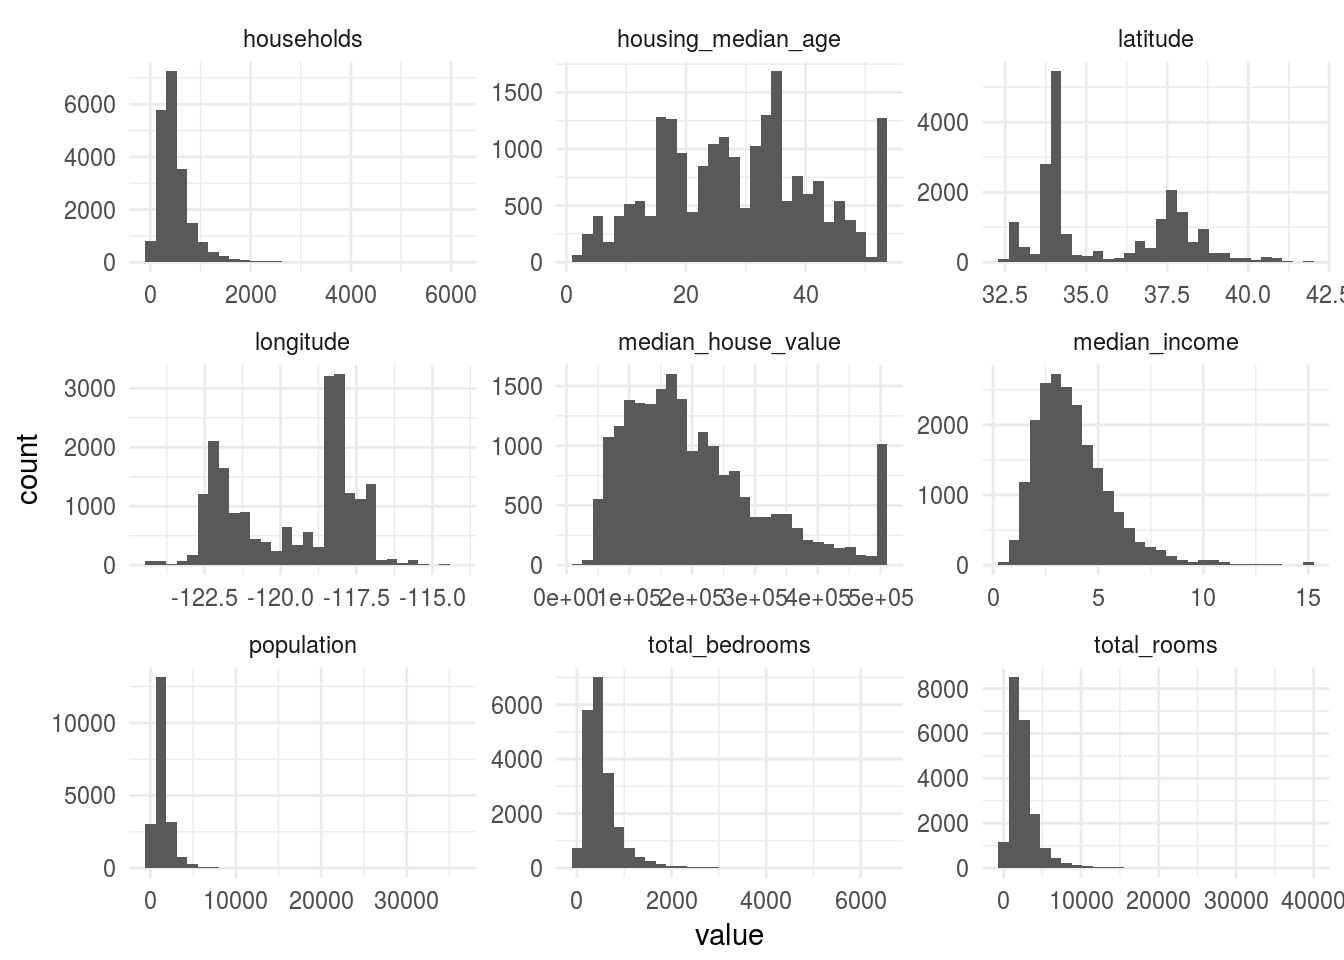
\includegraphics{mml-tutorial_files/figure-latex/gather-1.pdf}

\section{Spatial Visualizations}\label{spatial-visualizations}

The histograms of the longitude and latitude columns seem like they are
in some reasonable range of data. Let's visualize the locations.

\begin{Shaded}
\begin{Highlighting}[]
\NormalTok{housing }\OperatorTok\StringTok{ }\KeywordTok{ggplot}\NormalTok{(}\KeywordTok{aes}\NormalTok{(}\DataTypeTok{x =}\NormalTok{ longitude, }\DataTypeTok{y =}\NormalTok{ latitude)) }\OperatorTok{+}\StringTok{ }
\StringTok{  }\KeywordTok{geom_point}\NormalTok{()}
\end{Highlighting}
\end{Shaded}

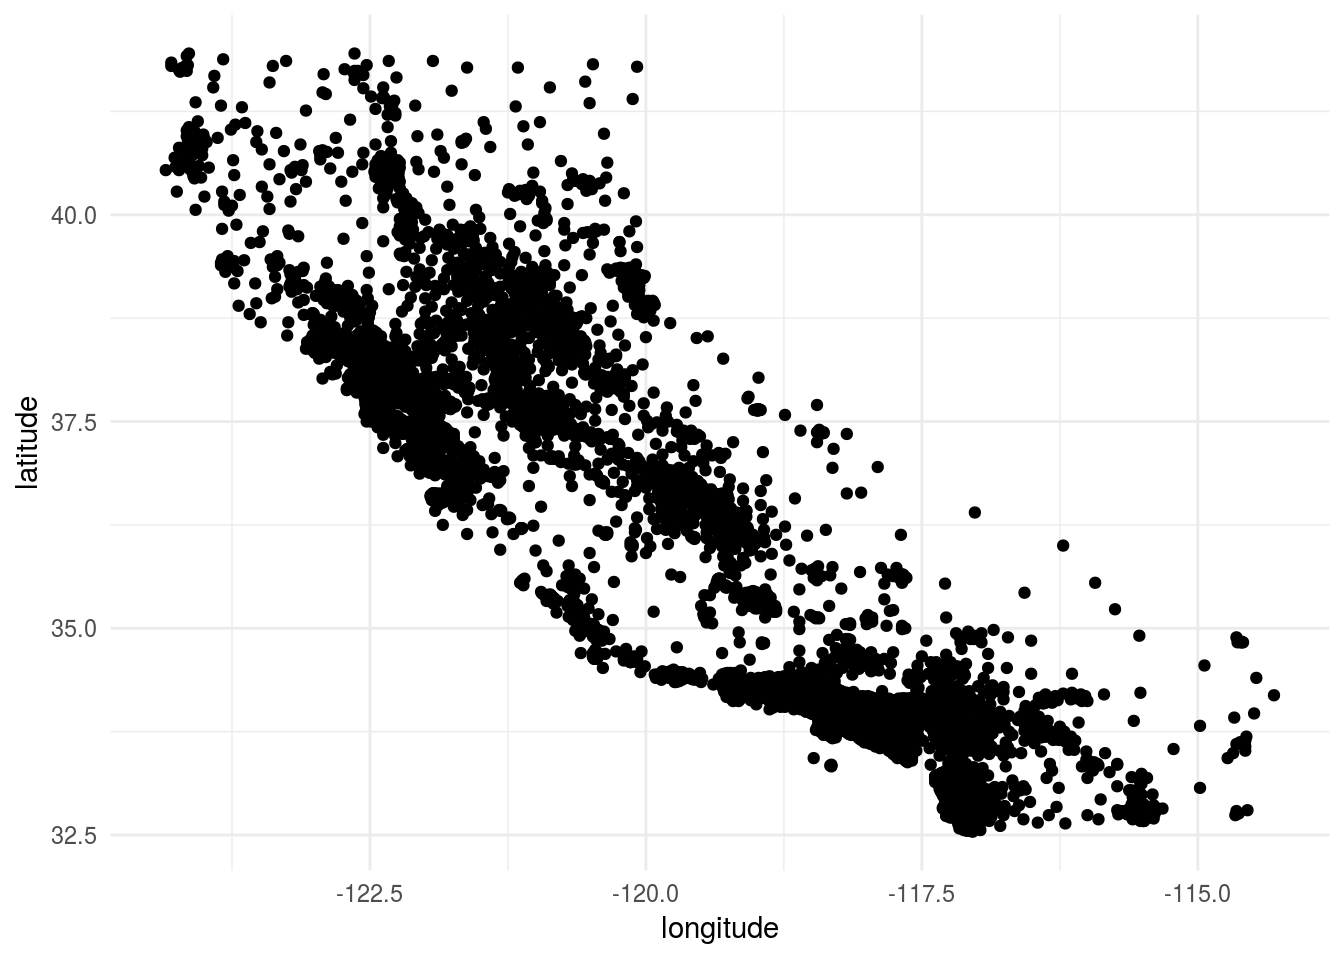
\includegraphics{mml-tutorial_files/figure-latex/spatial-visuals-1.pdf}

Looks indeed like California!

We can improve this chart in many ways. Let's first add some
transparency so we can get a better sense of the \emph{density} of
points:

\begin{Shaded}
\begin{Highlighting}[]
\NormalTok{housing }\OperatorTok\StringTok{ }\KeywordTok{ggplot}\NormalTok{(}\KeywordTok{aes}\NormalTok{(}\DataTypeTok{x =}\NormalTok{ longitude, }\DataTypeTok{y =}\NormalTok{ latitude)) }\OperatorTok{+}\StringTok{ }
\StringTok{  }\KeywordTok{geom_point}\NormalTok{(}\DataTypeTok{alpha =} \FloatTok{0.15}\NormalTok{)}
\end{Highlighting}
\end{Shaded}

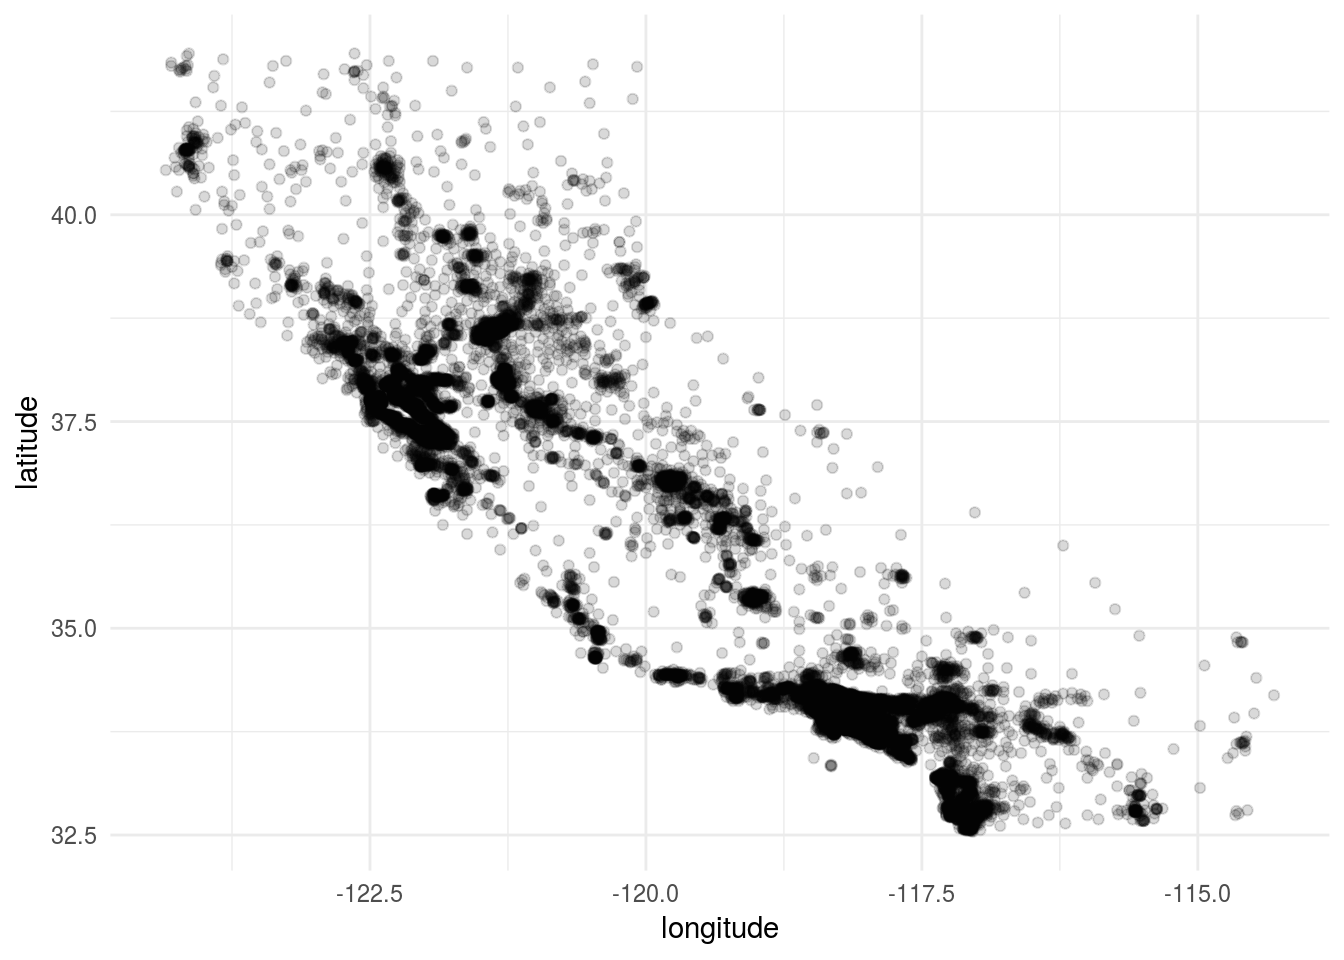
\includegraphics{mml-tutorial_files/figure-latex/alpha-1.pdf}

Nice, we can already see some dense clusters for higher population
regions like the Bay Area, Sacramento and Los Angeles.

Let's add some additional attributes, like the population:

\begin{Shaded}
\begin{Highlighting}[]
\NormalTok{housing }\OperatorTok\StringTok{ }\KeywordTok{ggplot}\NormalTok{(}\KeywordTok{aes}\NormalTok{(}\DataTypeTok{x =}\NormalTok{ longitude, }\DataTypeTok{y =}\NormalTok{ latitude,}
                       \DataTypeTok{size =}\NormalTok{ population)) }\OperatorTok{+}\StringTok{ }
\StringTok{  }\KeywordTok{geom_point}\NormalTok{(}\DataTypeTok{alpha =} \FloatTok{0.15}\NormalTok{)}
\end{Highlighting}
\end{Shaded}

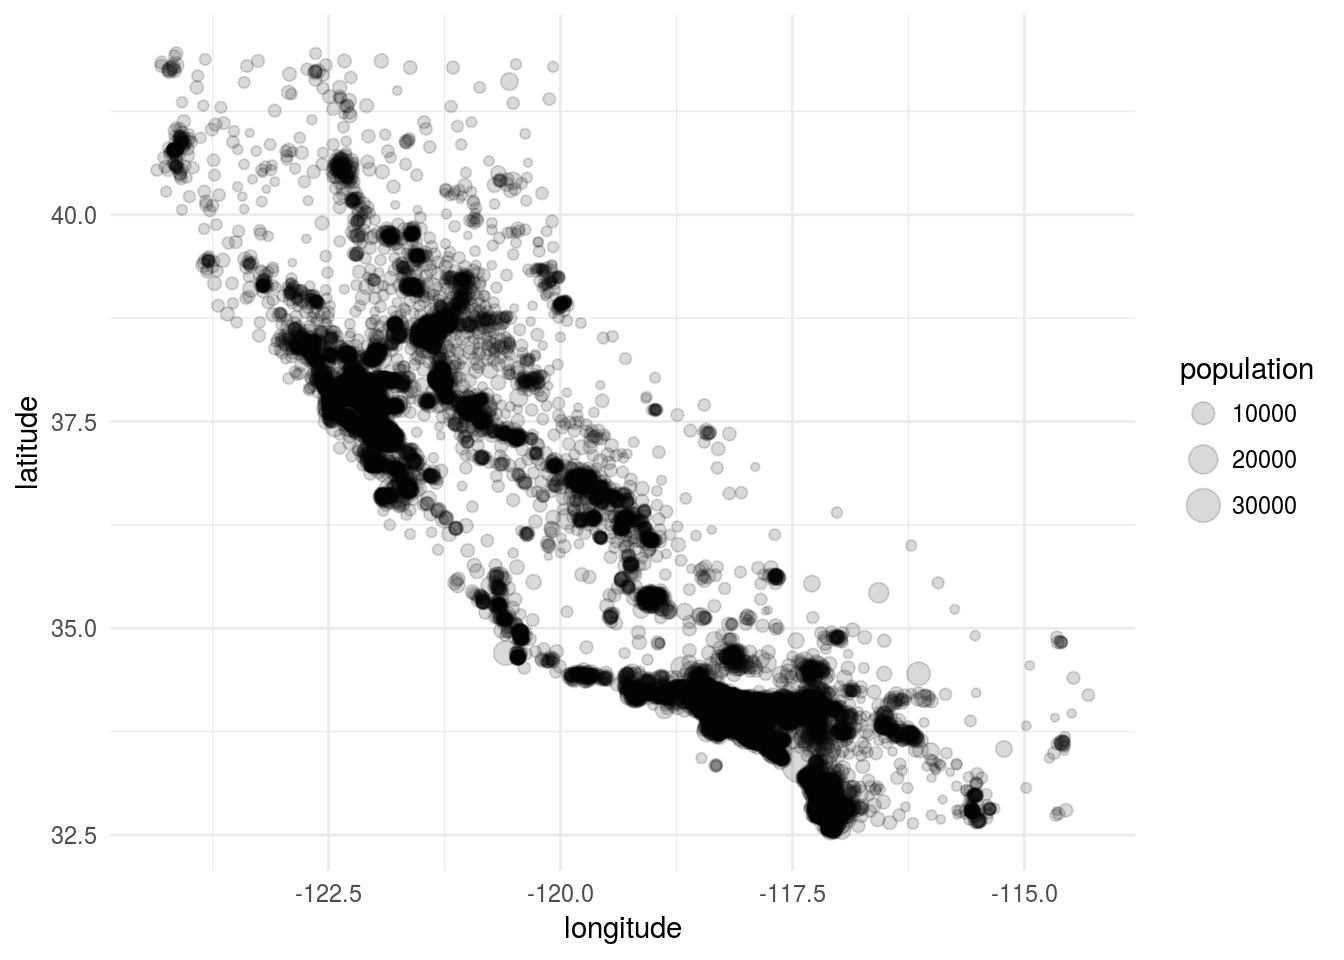
\includegraphics{mml-tutorial_files/figure-latex/population-1.pdf}

And now let's see if we can add a gradient fill for another numeric
value, like the median housing price:

\begin{Shaded}
\begin{Highlighting}[]
\NormalTok{housing }\OperatorTok\StringTok{ }\KeywordTok{ggplot}\NormalTok{(}\KeywordTok{aes}\NormalTok{(}\DataTypeTok{x =}\NormalTok{ longitude, }\DataTypeTok{y =}\NormalTok{ latitude,}
                       \DataTypeTok{size =}\NormalTok{ population,}
                       \DataTypeTok{colour =}\NormalTok{ median_house_value)) }\OperatorTok{+}\StringTok{ }
\StringTok{  }\KeywordTok{geom_point}\NormalTok{(}\DataTypeTok{alpha =} \FloatTok{0.095}\NormalTok{)}
\end{Highlighting}
\end{Shaded}

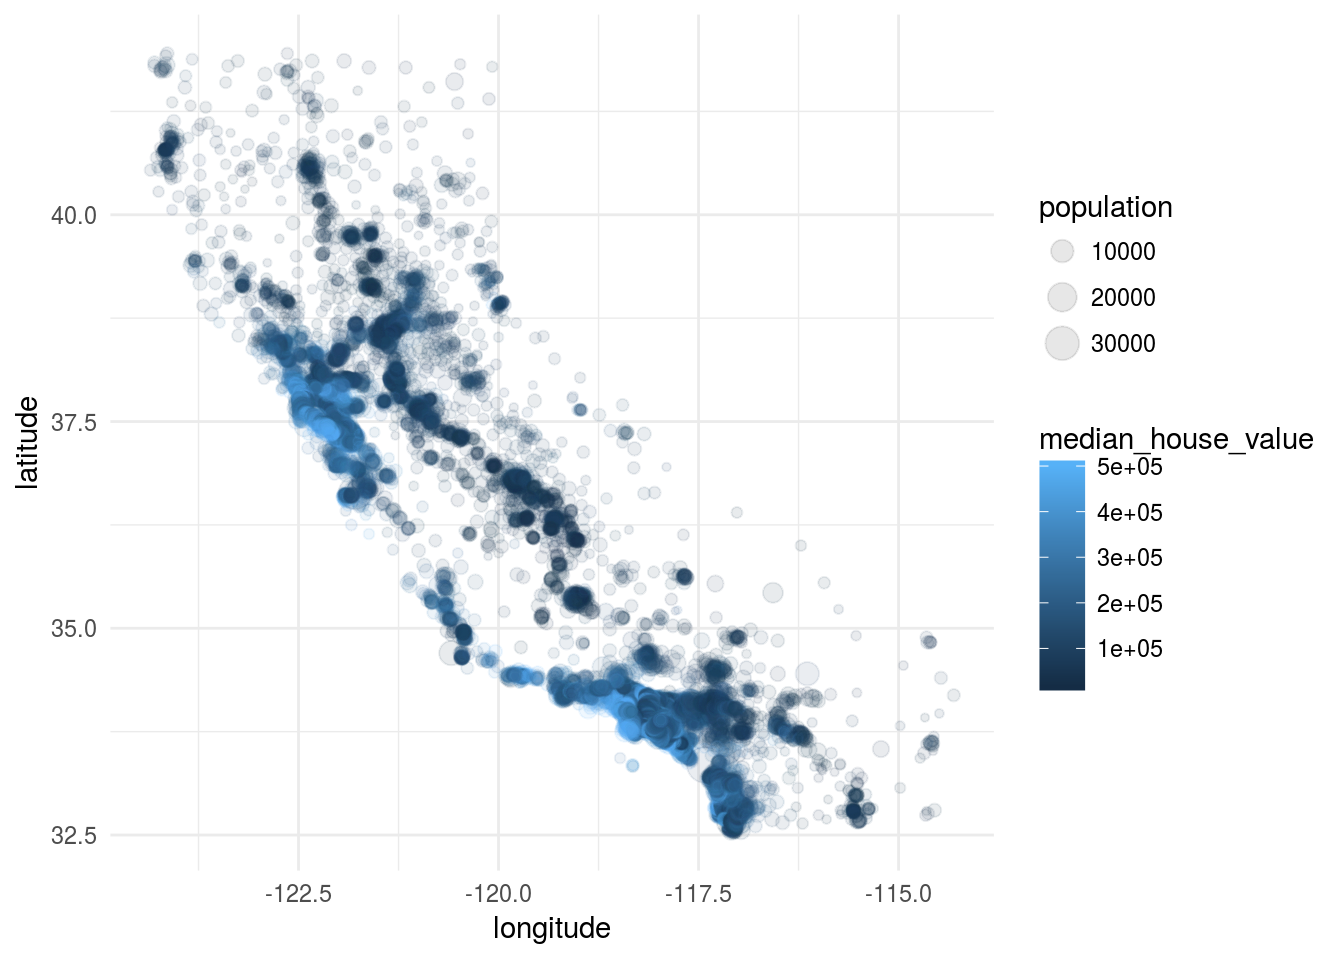
\includegraphics{mml-tutorial_files/figure-latex/gradient-fill-1.pdf}

Interesting, we can definitely see the higher price ranges in LA and the
Bay Area. Let's see if we can change the colour scheme to get an even
better visualization:

\begin{Shaded}
\begin{Highlighting}[]
\NormalTok{housing }\OperatorTok\StringTok{ }\KeywordTok{ggplot}\NormalTok{(}\KeywordTok{aes}\NormalTok{(}\DataTypeTok{x =}\NormalTok{ longitude, }\DataTypeTok{y =}\NormalTok{ latitude,}
                       \DataTypeTok{size =}\NormalTok{ population,}
                       \DataTypeTok{colour =}\NormalTok{ median_house_value)) }\OperatorTok{+}\StringTok{ }
\StringTok{  }\KeywordTok{geom_point}\NormalTok{(}\DataTypeTok{alpha =} \FloatTok{0.095}\NormalTok{) }\OperatorTok{+}
\StringTok{  }\KeywordTok{scale_colour_gradient}\NormalTok{(}\DataTypeTok{low =} \StringTok{"yellow"}\NormalTok{, }\DataTypeTok{high =} \StringTok{"red"}\NormalTok{)}
\end{Highlighting}
\end{Shaded}

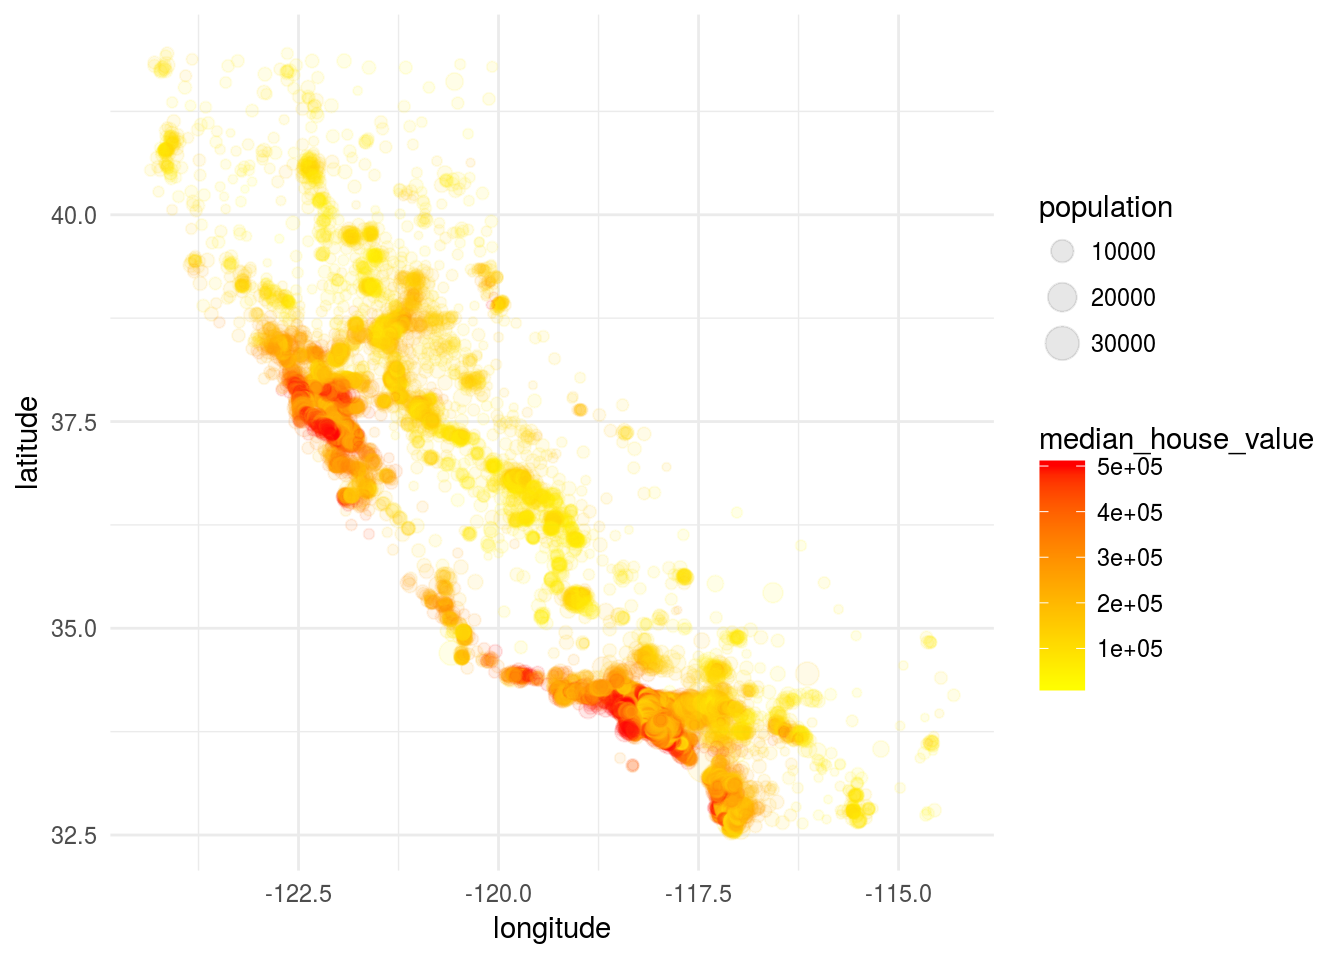
\includegraphics{mml-tutorial_files/figure-latex/colour-1.pdf}

If you want to plot the points on top of an actual polygon of the state
map, you can do that using \texttt{geom\_map} and using the
\texttt{map\_data} function in ggplot2. I find it a bit messy, but it
might be worthwile if you are plotting various regions/states.

While we're at it, let's put some final themes on our plot to make it
more aesthetically pleasing.

\begin{Shaded}
\begin{Highlighting}[]
\NormalTok{housing }\OperatorTok\StringTok{ }
\StringTok{  }\KeywordTok{mutate}\NormalTok{(}\DataTypeTok{state =} \StringTok{"california"}\NormalTok{) }\OperatorTok\StringTok{ }
\StringTok{  }\KeywordTok{ggplot}\NormalTok{(}\KeywordTok{aes}\NormalTok{(}\DataTypeTok{x =}\NormalTok{ longitude, }\DataTypeTok{y =}\NormalTok{ latitude,}
             \DataTypeTok{size =}\NormalTok{ population,}
             \DataTypeTok{colour =}\NormalTok{ median_house_value)) }\OperatorTok{+}
\StringTok{  }\KeywordTok{geom_map}\NormalTok{(}\DataTypeTok{map =} \KeywordTok{filter}\NormalTok{(}\KeywordTok{map_data}\NormalTok{(}\StringTok{"state"}\NormalTok{), region }\OperatorTok{==}\StringTok{ "california"}\NormalTok{),}
           \KeywordTok{aes}\NormalTok{(}\DataTypeTok{map_id =}\NormalTok{ state), }
           \DataTypeTok{fill =} \StringTok{"lightgrey"}\NormalTok{,}
           \DataTypeTok{colour =} \StringTok{"lightgrey"}\NormalTok{) }\OperatorTok{+}
\StringTok{  }\KeywordTok{geom_point}\NormalTok{(}\DataTypeTok{alpha =} \FloatTok{0.1}\NormalTok{) }\OperatorTok{+}
\StringTok{  }\KeywordTok{theme}\NormalTok{(}\DataTypeTok{panel.grid.major =} \KeywordTok{element_blank}\NormalTok{(),}
        \DataTypeTok{panel.grid.minor =} \KeywordTok{element_blank}\NormalTok{()) }\OperatorTok{+}\StringTok{ }
\StringTok{  }\KeywordTok{scale_size_continuous}\NormalTok{(}\DataTypeTok{labels =}\NormalTok{ scales}\OperatorTok{::}\NormalTok{comma) }\OperatorTok{+}
\StringTok{  }\KeywordTok{scale_colour_gradient}\NormalTok{(}\DataTypeTok{low =} \StringTok{"yellow"}\NormalTok{, }\DataTypeTok{high =} \StringTok{"red"}\NormalTok{,}
                        \DataTypeTok{labels =}\NormalTok{ scales}\OperatorTok{::}\NormalTok{dollar)}
\end{Highlighting}
\end{Shaded}

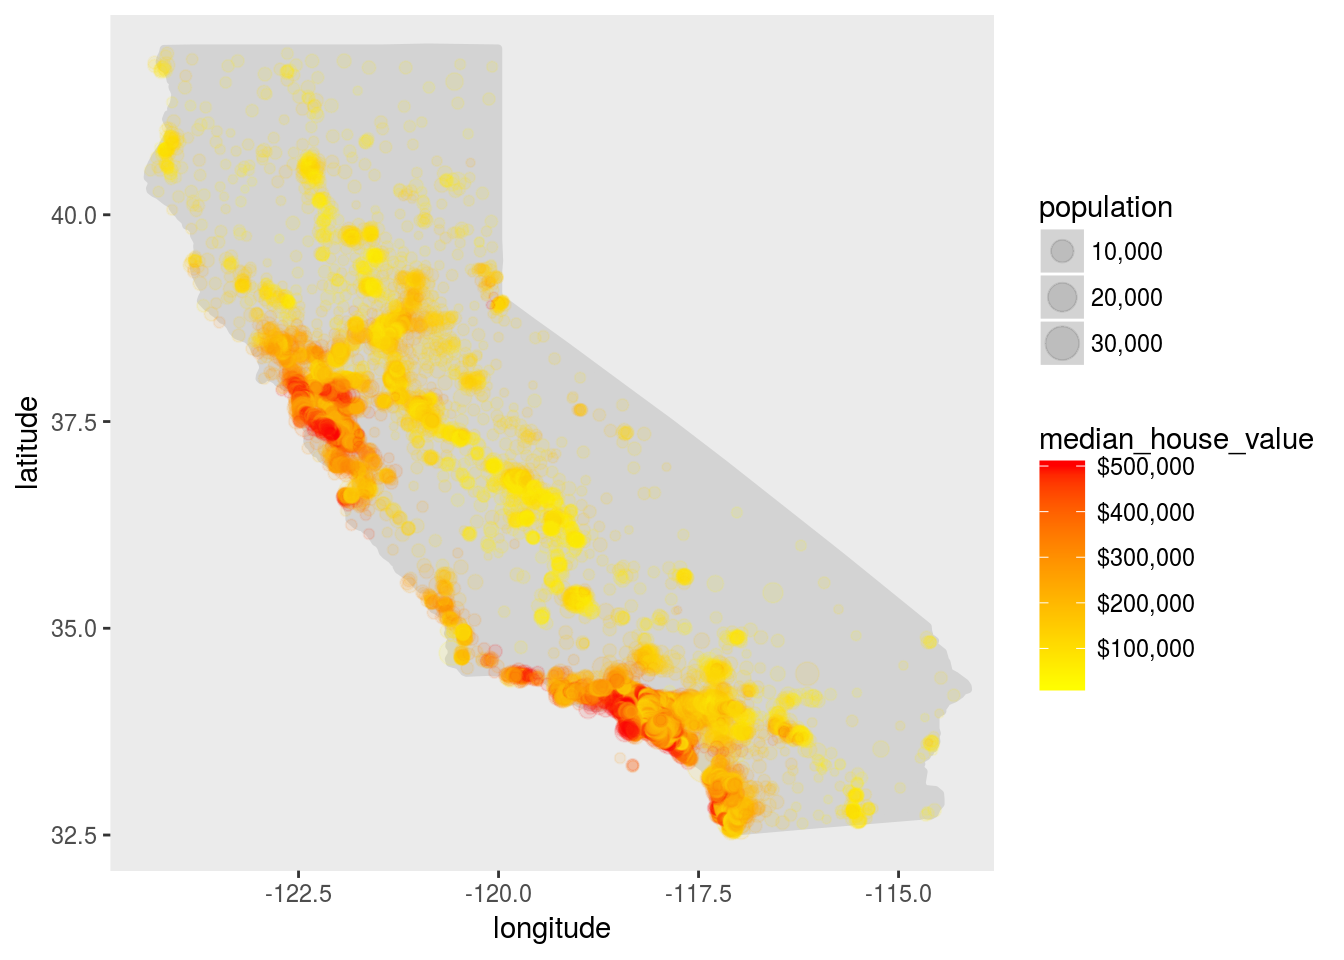
\includegraphics{mml-tutorial_files/figure-latex/geommap-1.pdf}

\section{Exercises}\label{exercises}

\begin{enumerate}
\def\labelenumi{\arabic{enumi}.}
\tightlist
\item
  How does proximity to the ocean effect median house values? Try to
  visualize housing prices the above using the ocean proximity variable
  as the colour/fill aesthetic and median\_house\_value as the size
  aesthetic.
\item
  We saw that faceting could allow us to compare distributions rather
  easily. Try a facetted plot where you facet by quantiles of the
  \texttt{median\_income} column. This will allow you to compare the
  distribution of housing values, populations/demographics across
  different income groups. The \texttt{dplyr::mutate},
  \texttt{stats::quntile}, and \texttt{ggplot2::facet\_wrap} functions
  should be useful here.
\end{enumerate}

\chapter{Regression Models}\label{regression-models}

\section{Splitting into Train and Test
Sets}\label{splitting-into-train-and-test-sets}

Let's sample our data into train and test sets. In order to do this
efficiently, we will use the \texttt{RevoScaleR} package.

We'll first create a \texttt{RxXdfData} object, which is a more
efficient and scalable data structure than R \texttt{data.frames}. Their
primary distinction is that they do not reside in memory, but on-disk.

\begin{Shaded}
\begin{Highlighting}[]
\KeywordTok{library}\NormalTok{(tidyverse)}
\KeywordTok{library}\NormalTok{(dplyrXdf)}
\KeywordTok{library}\NormalTok{(foreach)}
\KeywordTok{library}\NormalTok{(doRSR)}
\KeywordTok{library}\NormalTok{(MicrosoftML)}
\KeywordTok{theme_set}\NormalTok{(}\KeywordTok{theme_minimal}\NormalTok{())}

\NormalTok{out_xdf <-}\StringTok{ }\KeywordTok{file.path}\NormalTok{(}
                     \StringTok{"data"}\NormalTok{,}
                     \StringTok{"housing.xdf"}\NormalTok{)}

\NormalTok{housing_xdf <-}\StringTok{ }\KeywordTok{rxDataStep}\NormalTok{(}\DataTypeTok{inData =}\NormalTok{ housing,}
                          \DataTypeTok{outFile =}\NormalTok{ out_xdf,}
                          \DataTypeTok{maxRowsByCols =} \KeywordTok{nrow}\NormalTok{(housing)}\OperatorTok{*}\KeywordTok{ncol}\NormalTok{(housing),}
                          \DataTypeTok{rowsPerRead =} \DecValTok{5000}\NormalTok{,}
                          \DataTypeTok{overwrite =} \OtherTok{TRUE}\NormalTok{)}

\NormalTok{housing_xdf }\OperatorTok\StringTok{ }\KeywordTok{factorise}\NormalTok{(ocean_proximity) }\OperatorTok\StringTok{ }
\StringTok{  }\KeywordTok{persist}\NormalTok{(out_xdf, }\DataTypeTok{overwrite =} \OtherTok{TRUE}\NormalTok{)}
\end{Highlighting}
\end{Shaded}

The \texttt{RevoScaleR} and \texttt{MicrosoftML} functions are primarily
prefixed with \texttt{rx}. In this function below, we will use the
\texttt{rxSplit} function to split our data into train and test sets.
Observe that since our data is now on-disk, and compromises of multiple
blocks, we have to use the \texttt{.rxNumRows} argument to inform the
session how many rows are currently being processed in the current
block:

\begin{Shaded}
\begin{Highlighting}[]
\NormalTok{split_xdf <-}\StringTok{ }\ControlFlowTok{function}\NormalTok{(data) \{}

\NormalTok{    splits <-}\StringTok{ }\KeywordTok{rxSplit}\NormalTok{(data,}
                      \DataTypeTok{outFileSuffixes =} \KeywordTok{c}\NormalTok{(}\StringTok{"Train"}\NormalTok{, }\StringTok{"Test"}\NormalTok{, }\StringTok{"Validate"}\NormalTok{),}
                         \DataTypeTok{splitByFactor =} \StringTok{"splitVar"}\NormalTok{,}
                         \DataTypeTok{overwrite =} \OtherTok{TRUE}\NormalTok{,}
                         \DataTypeTok{transforms =} \KeywordTok{list}\NormalTok{(}\DataTypeTok{splitVar =} \KeywordTok{factor}\NormalTok{(}
                           \KeywordTok{sample}\NormalTok{(}\KeywordTok{c}\NormalTok{(}\StringTok{"Train"}\NormalTok{, }\StringTok{"Test"}\NormalTok{, }\StringTok{"Validate"}\NormalTok{),}
                                  \DataTypeTok{size =}\NormalTok{ .rxNumRows,}
                                  \DataTypeTok{replace =} \OtherTok{TRUE}\NormalTok{,}
                                  \DataTypeTok{prob =} \KeywordTok{c}\NormalTok{(}\FloatTok{0.65}\NormalTok{, }\FloatTok{0.25}\NormalTok{, }\FloatTok{0.1}\NormalTok{)),}
                           \DataTypeTok{levels =} \KeywordTok{c}\NormalTok{(}\StringTok{"Train"}\NormalTok{, }\StringTok{"Test"}\NormalTok{, }\StringTok{"Validate"}\NormalTok{))),}
                         \DataTypeTok{rngSeed =} \DecValTok{123}\NormalTok{,}
                         \DataTypeTok{consoleOutput =} \OtherTok{TRUE}\NormalTok{)}
  \KeywordTok{return}\NormalTok{(splits)}
\NormalTok{\}}


\NormalTok{splits <-}\StringTok{ }\KeywordTok{split_xdf}\NormalTok{(housing_xdf)}
\KeywordTok{names}\NormalTok{(splits) <-}\StringTok{ }\KeywordTok{c}\NormalTok{(}\StringTok{"train"}\NormalTok{, }\StringTok{"test"}\NormalTok{, }\StringTok{"validate"}\NormalTok{)}
\end{Highlighting}
\end{Shaded}

Now that we have our train and test sets, we can conduct begin to train
our models.

\section{Training Regression
Learners}\label{training-regression-learners}

Let's train our first regression model.

We can start with the a \texttt{glm} model. GLMs, short for generalized
linear models, are a general class of linear algorithms. In this
exercise, our goal is to predict the median housing value given the
other variables.

\begin{Shaded}
\begin{Highlighting}[]
\NormalTok{lin_mod <-}\StringTok{ }\KeywordTok{rxLinMod}\NormalTok{(median_house_value }\OperatorTok{~}\StringTok{ }\NormalTok{housing_median_age }\OperatorTok{+}\StringTok{ }\NormalTok{total_rooms }\OperatorTok{+}\StringTok{ }\NormalTok{total_bedrooms }\OperatorTok{+}
\StringTok{                      }\NormalTok{population }\OperatorTok{+}\StringTok{ }\NormalTok{households }\OperatorTok{+}\StringTok{ }\NormalTok{median_income }\OperatorTok{+}\StringTok{ }\NormalTok{ocean_proximity,}
                    \DataTypeTok{data =}\NormalTok{ splits}\OperatorTok{$}\NormalTok{train)}
\end{Highlighting}
\end{Shaded}

That was pretty easy, but let's generalize our approach so that we can
estimate a variety of models quickly and efficiently.

First, we'll create a wrapper function to automatically create our model
matrix for us dynamically from our data.

\begin{Shaded}
\begin{Highlighting}[]
\NormalTok{make_form <-}\StringTok{ }\ControlFlowTok{function}\NormalTok{(}\DataTypeTok{xdf =}\NormalTok{ housing_xdf,}
                      \DataTypeTok{resp_var =} \StringTok{"median_house_value"}\NormalTok{,}
                      \DataTypeTok{vars_to_skip =} \KeywordTok{c}\NormalTok{(}\StringTok{"splitVar"}\NormalTok{, }\StringTok{"longitude"}\NormalTok{, }
                                       \StringTok{"latitude"}\NormalTok{)) \{}
  
  \KeywordTok{library}\NormalTok{(stringr)}
  
\NormalTok{  non_incl <-}\StringTok{ }\KeywordTok{paste}\NormalTok{(vars_to_skip, }\DataTypeTok{collapse =} \StringTok{"|"}\NormalTok{)}
  
\NormalTok{  x_names <-}\StringTok{ }\KeywordTok{names}\NormalTok{(xdf)}
  
\NormalTok{  features <-}\StringTok{ }\NormalTok{x_names[}\OperatorTok{!}\KeywordTok{str_detect}\NormalTok{(x_names, resp_var)]}
\NormalTok{  features <-}\StringTok{ }\NormalTok{features[}\OperatorTok{!}\KeywordTok{str_detect}\NormalTok{(features, non_incl)]}
  
\NormalTok{  form <-}\StringTok{ }\KeywordTok{as.formula}\NormalTok{(}\KeywordTok{paste}\NormalTok{(resp_var, }\KeywordTok{paste0}\NormalTok{(features, }\DataTypeTok{collapse =} \StringTok{" + "}\NormalTok{),}
                           \DataTypeTok{sep  =} \StringTok{" ~ "}\NormalTok{))}
  
  \KeywordTok{return}\NormalTok{(form)}
\NormalTok{\}}

\KeywordTok{make_form}\NormalTok{(}\DataTypeTok{xdf =}\NormalTok{ splits}\OperatorTok{$}\NormalTok{train)}
\end{Highlighting}
\end{Shaded}

\begin{verbatim}
## median_house_value ~ housing_median_age + total_rooms + total_bedrooms + 
##     population + households + median_income + ocean_proximity
## <environment: 0xbbeb960>
\end{verbatim}

Now let's create a modeling wrapper, which will take our dataset, a
formula, and a model, and train it for us.

\begin{Shaded}
\begin{Highlighting}[]
\NormalTok{estimate_model <-}\StringTok{ }\ControlFlowTok{function}\NormalTok{(}\DataTypeTok{xdf_data =}\NormalTok{ splits}\OperatorTok{$}\NormalTok{train,}
                           \DataTypeTok{form =} \KeywordTok{make_form}\NormalTok{(}\DataTypeTok{xdf =}\NormalTok{ xdf_data),}
                           \DataTypeTok{model =}\NormalTok{ rxLogit, ...) \{}
  
\NormalTok{  rx_model <-}\StringTok{ }\KeywordTok{model}\NormalTok{(form, }\DataTypeTok{data =}\NormalTok{ xdf_data, ...)}
  
  \KeywordTok{return}\NormalTok{(rx_model)}
  
  
\NormalTok{\}}
\end{Highlighting}
\end{Shaded}

Now we can quickly iterate over our data and train models using
different learning algorithms. For example, the above example suffers
from the issue that we didn't scale our data prior to learning. This can
have an adverse effect on the optimization function of the learning
algorithm, as it'll favor the variables with more disperse scales.

We'll use the \href{http://dl.acm.org/citation.cfm?id=2783412}{SDCA -
Stochastic Dual Coordinate Ascent} learning algorithm, which
automatically applies a min-max scaling to our data prior to training.

\begin{Shaded}
\begin{Highlighting}[]
\NormalTok{sdca <-}\StringTok{ }\KeywordTok{estimate_model}\NormalTok{(}\DataTypeTok{model =}\NormalTok{ rxFastLinear, }\DataTypeTok{type =} \StringTok{"regression"}\NormalTok{)}
\end{Highlighting}
\end{Shaded}

\begin{verbatim}
## Automatically adding a MinMax normalization transform, use 'norm=Warn' or 'norm=No' to turn this behavior off.
## Using 2 threads to train.
## Automatically choosing a check frequency of 2.
## Warning: Skipped 128 instances with missing features/label during training
## Auto-tuning parameters: maxIterations = 110.
## Auto-tuning parameters: L2 = 0.0001.
## Auto-tuning parameters: L1Threshold (L1/L2) = 0.
## Using best model from iteration 78.
## Not training a calibrator because it is not needed.
## Elapsed time: 00:00:00.9279494
## Elapsed time: 00:00:00.0009998
\end{verbatim}

\begin{Shaded}
\begin{Highlighting}[]
\KeywordTok{summary}\NormalTok{(sdca)}
\end{Highlighting}
\end{Shaded}

\begin{verbatim}
## Call:
## model(formula = form, data = xdf_data, type = "regression")
## 
## SDCAR (RegressorTrainer) for: median_house_value~housing_median_age+total_rooms+total_bedrooms+population+households+median_income+ocean_proximity
## Data: xdf_data (RxXdfData Data Source)
## File name: /home/alizaidi/bookdown-demo/housing.splitVar.Train.xdf 
## 
## First 12 of 12 Non-zero Coefficients:
## (Bias): -32979.58
## population: -958475.9
## median_income: 562343.2
## total_bedrooms: 376008.2
## households: 238733.6
## ocean_proximity.ISLAND: 200716.1
## ocean_proximity.NEAR OCEAN: 86880.88
## ocean_proximity.NEAR BAY: 79374.24
## total_rooms: -74753.57
## ocean_proximity.<1H OCEAN: 73038.17
## housing_median_age: 47560.33
## ocean_proximity.INLAND: 4924.849
\end{verbatim}

\section{Scoring Our Data on the Test
Set}\label{scoring-our-data-on-the-test-set}

Now that we our model trained, we can score it on our test set.

Let's create a prediction XDF where we'll save our results to.

\begin{Shaded}
\begin{Highlighting}[]
\NormalTok{pred_xdf <-}\StringTok{ }\KeywordTok{file.path}\NormalTok{(}\StringTok{"/home"}\NormalTok{, }\KeywordTok{system}\NormalTok{(}\StringTok{"whoami"}\NormalTok{, }\DataTypeTok{intern =} \OtherTok{TRUE}\NormalTok{), }\StringTok{"scored.xdf"}\NormalTok{)}
\ControlFlowTok{if}\NormalTok{ (}\KeywordTok{file.exists}\NormalTok{(pred_xdf)) }\KeywordTok{file.remove}\NormalTok{(pred_xdf)}
\end{Highlighting}
\end{Shaded}

\begin{verbatim}
## [1] TRUE
\end{verbatim}

\begin{Shaded}
\begin{Highlighting}[]
\NormalTok{scored_xdf <-}\StringTok{ }\KeywordTok{RxXdfData}\NormalTok{(pred_xdf)}
\end{Highlighting}
\end{Shaded}

\begin{Shaded}
\begin{Highlighting}[]
\KeywordTok{rxPredict}\NormalTok{(lin_mod, }\DataTypeTok{data =}\NormalTok{ splits}\OperatorTok{$}\NormalTok{test, }
          \DataTypeTok{outData =}\NormalTok{ pred_xdf, }\DataTypeTok{writeModelVars =}\NormalTok{ T, }
          \DataTypeTok{predVarNames =} \KeywordTok{c}\NormalTok{(}\StringTok{"linmod"}\NormalTok{), }\DataTypeTok{overwrite =}\NormalTok{ T)}
\KeywordTok{rxGetInfo}\NormalTok{(pred_xdf)}
\end{Highlighting}
\end{Shaded}

\begin{verbatim}
## File name: /home/alizaidi/scored.xdf 
## Number of observations: 5003 
## Number of variables: 9 
## Number of blocks: 5 
## Compression type: zlib
\end{verbatim}

\begin{Shaded}
\begin{Highlighting}[]
\KeywordTok{rxLinePlot}\NormalTok{(linmod }\OperatorTok{~}\StringTok{ }\NormalTok{median_house_value, }\DataTypeTok{data =}\NormalTok{ pred_xdf, }\DataTypeTok{type =} \StringTok{"p"}\NormalTok{)}
\end{Highlighting}
\end{Shaded}

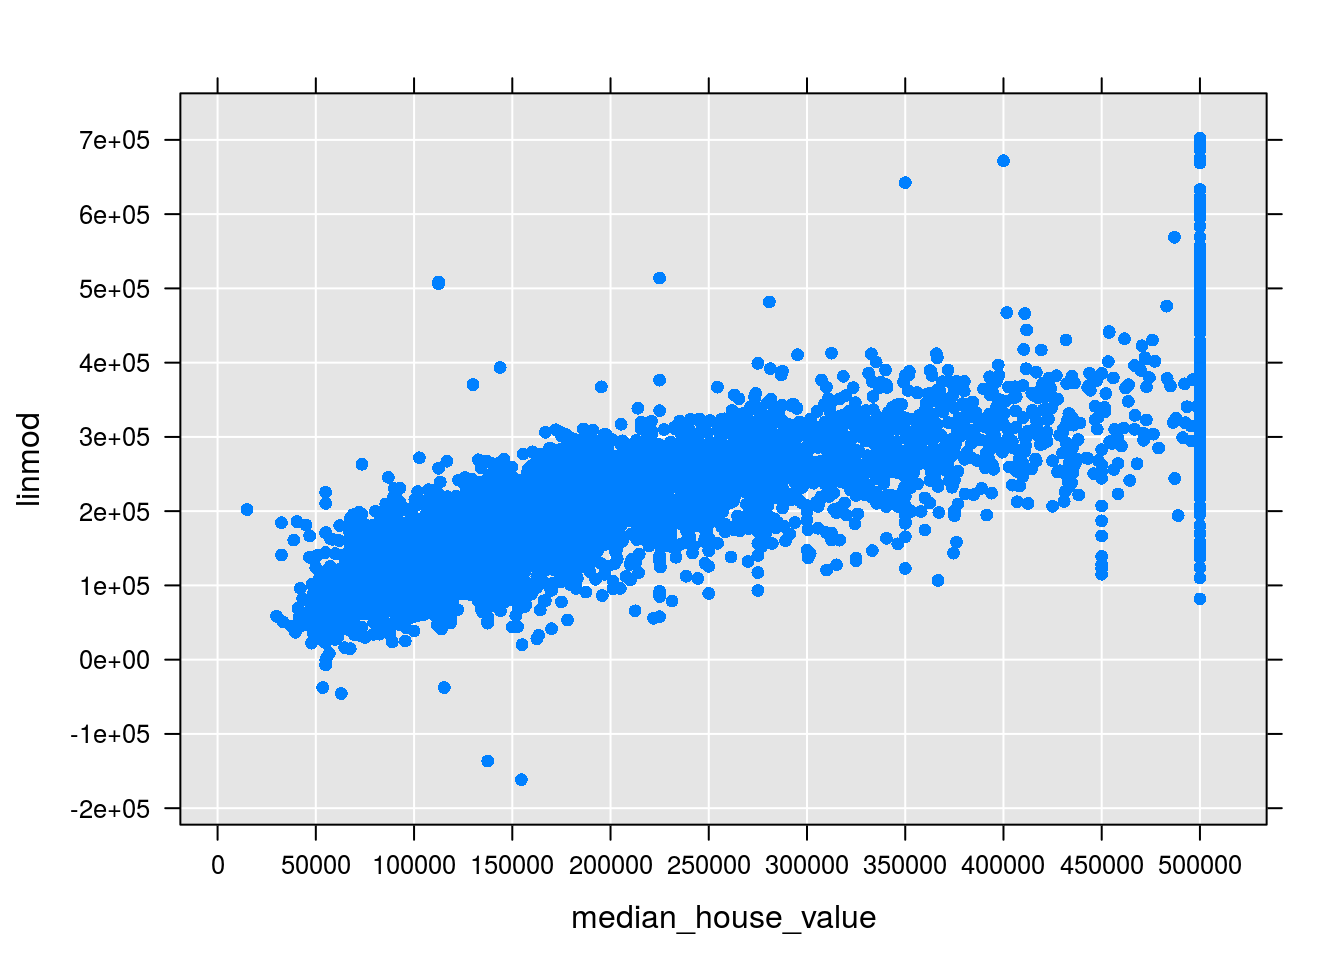
\includegraphics{mml-tutorial_files/figure-latex/predict-1.pdf}

Let's also score our SDCA model:

\begin{Shaded}
\begin{Highlighting}[]
\KeywordTok{rxPredict}\NormalTok{(sdca, }\DataTypeTok{data =}\NormalTok{ splits}\OperatorTok{$}\NormalTok{test, }
          \DataTypeTok{outData =}\NormalTok{ pred_xdf, }\DataTypeTok{writeModelVars =}\NormalTok{ T)}
\end{Highlighting}
\end{Shaded}

\begin{verbatim}
## Elapsed time: 00:00:00.0249283
\end{verbatim}

\begin{Shaded}
\begin{Highlighting}[]
\CommentTok{# rxGetInfo(pred_xdf, numRows = 2)}
\KeywordTok{rxLinePlot}\NormalTok{(Score }\OperatorTok{~}\StringTok{ }\NormalTok{median_house_value, }\DataTypeTok{data =}\NormalTok{ pred_xdf, }\DataTypeTok{type =} \StringTok{"p"}\NormalTok{)}
\end{Highlighting}
\end{Shaded}

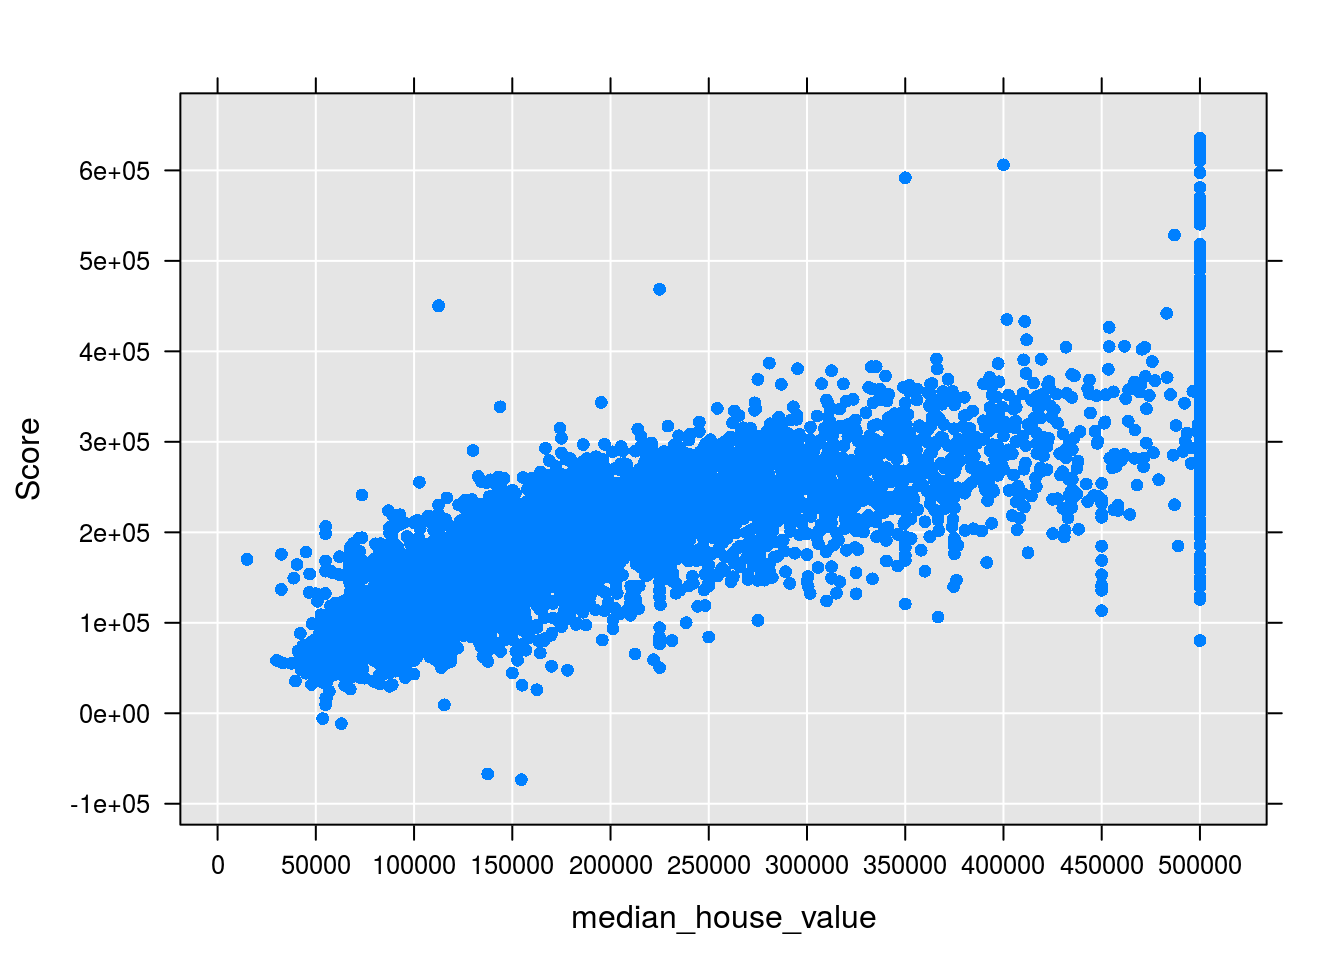
\includegraphics{mml-tutorial_files/figure-latex/sdca-preds-1.pdf}

\section{Training Many Models
Concurrently}\label{training-many-models-concurrently}

Let's take our functions and train multiple models in parallel. We have
already trained two linear models. Let's add two ensemble tree
algorithms to the mix, \texttt{rxBTrees}, and simultaneously train a
random forest using \texttt{rxDForest}.

To run them in parallel, we can use the foreach package with a local
parallel backend.

\begin{Shaded}
\begin{Highlighting}[]
\KeywordTok{rxSetComputeContext}\NormalTok{(}\KeywordTok{RxLocalParallel}\NormalTok{())}
\KeywordTok{registerDoRSR}\NormalTok{(}\DataTypeTok{computeContext =} \KeywordTok{rxGetComputeContext}\NormalTok{())}

\NormalTok{models <-}\StringTok{ }\KeywordTok{list}\NormalTok{(}\StringTok{"btrees"}\NormalTok{ =}\StringTok{ }\NormalTok{rxBTrees, }
               \StringTok{"forest"}\NormalTok{ =}\StringTok{ }\NormalTok{rxDForest)}
\NormalTok{models <-}\StringTok{ }\KeywordTok{foreach}\NormalTok{(}\DataTypeTok{i =}\NormalTok{ models) }\OperatorTok\StringTok{ }\KeywordTok{estimate_model}\NormalTok{(}\DataTypeTok{model =}\NormalTok{ i)}
\KeywordTok{names}\NormalTok{(models) <-}\StringTok{ }\KeywordTok{c}\NormalTok{(}\StringTok{"btrees"}\NormalTok{, }\StringTok{"forest"}\NormalTok{)}
\NormalTok{models}
\end{Highlighting}
\end{Shaded}

\begin{verbatim}
## $btrees
## 
## Call:
## model(formula = form, data = xdf_data)
## 
## 
##       Loss function of boosted trees: bernoulli 
##        Number of boosting iterations: 10 
## No. of variables tried at each split: 2 
## 
##             OOB estimate of deviance: NA 
## 
## $forest
## 
## Call:
## model(formula = form, data = xdf_data)
## 
## 
##              Type of decision forest: anova 
##                      Number of trees: 10 
## No. of variables tried at each split: 2 
## 
##           Mean of squared residuals: 4563008000
##                     % Var explained: 66
\end{verbatim}

\begin{Shaded}
\begin{Highlighting}[]
\KeywordTok{lapply}\NormalTok{(models, summary)}
\end{Highlighting}
\end{Shaded}

\begin{verbatim}
## $btrees
##           Length Class      Mode     
## ntree      1     -none-     numeric  
## mtry       1     -none-     numeric  
## type       1     -none-     character
## forest    10     -none-     list     
## oob.err    4     data.frame list     
## init.pred  1     -none-     numeric  
## params    65     -none-     list     
## formula    3     formula    call     
## call       3     -none-     call     
## 
## $forest
##         Length Class      Mode     
## ntree    1     -none-     numeric  
## mtry     1     -none-     numeric  
## type     1     -none-     character
## forest  10     -none-     list     
## oob.err  4     data.frame list     
## params  65     -none-     list     
## formula  3     formula    call     
## call     3     -none-     call
\end{verbatim}

\section{Exercise}\label{exercise}

\begin{enumerate}
\def\labelenumi{\arabic{enumi}.}
\tightlist
\item
  Use the \texttt{rxDTree} function to sit a single regression tree to
  this dataset.
\item
  Visualize the fit of your decision tree using the
  \texttt{RevoTreeView} library and it's \texttt{createTreeView} and
  \texttt{plot} functions.
\end{enumerate}

\chapter{Classification Models for Computer
Vision}\label{classification-models-for-computer-vision}

\section{Hand-Written Digit
Classifiation}\label{hand-written-digit-classifiation}

In this module, we will examine the
\href{http://yann.lecun.com/exdb/mnist/}{MNIST} dataset, which is a set
of 70,000 images of digits handwritten by high school students and
employees of the US Census Bureau.

MNIST is considered the ``hello-world'' of the machine-learning world,
and is often a good place to start for understanding classification
algorithms.

Let's load the MNIST dataset.

\begin{Shaded}
\begin{Highlighting}[]
\KeywordTok{library}\NormalTok{(MicrosoftML)}
\KeywordTok{library}\NormalTok{(tidyverse)}
\KeywordTok{library}\NormalTok{(magrittr)}
\KeywordTok{library}\NormalTok{(dplyrXdf)}
\KeywordTok{theme_set}\NormalTok{(}\KeywordTok{theme_minimal}\NormalTok{())}

\NormalTok{mnist_xdf <-}\StringTok{ }\KeywordTok{file.path}\NormalTok{(}\StringTok{"data"}\NormalTok{, }\StringTok{"MNIST.xdf"}\NormalTok{)}
\NormalTok{mnist_xdf <-}\StringTok{ }\KeywordTok{RxXdfData}\NormalTok{(mnist_xdf)}
\end{Highlighting}
\end{Shaded}

Let's take a look at the data:

\begin{Shaded}
\begin{Highlighting}[]
\KeywordTok{rxGetInfo}\NormalTok{(mnist_xdf)}
\end{Highlighting}
\end{Shaded}

\begin{verbatim}
## File name: /home/alizaidi/bookdown-demo/data/MNIST.xdf 
## Number of observations: 70000 
## Number of variables: 786 
## Number of blocks: 7 
## Compression type: zlib
\end{verbatim}

Our dataset contains 70K records, and 786 columns. There are actually
784 features, because each image in the dataset is a 28x28 pixel image.
The two additional columns are for the label, and a column with a
pre-sampled train and test split.

\section{Visualizing Digits}\label{visualizing-digits}

Let's make some visualizations to examine the MNIST data and see what we
can use for a classifier to classify the digits.

\begin{Shaded}
\begin{Highlighting}[]
\NormalTok{mnist_df <-}\StringTok{ }\KeywordTok{rxDataStep}\NormalTok{(}\DataTypeTok{inData =}\NormalTok{ mnist_xdf, }\DataTypeTok{outFile =} \OtherTok{NULL}\NormalTok{,}
                       \DataTypeTok{maxRowsByCols =} \KeywordTok{nrow}\NormalTok{(mnist_xdf)}\OperatorTok{*}\KeywordTok{ncol}\NormalTok{(mnist_xdf)) }\OperatorTok\StringTok{ }\NormalTok{tbl_df}
\end{Highlighting}
\end{Shaded}

Let's see the average for each digit:

\begin{Shaded}
\begin{Highlighting}[]
\NormalTok{mnist_df }\OperatorTok\StringTok{ }
\StringTok{  }\KeywordTok{keep}\NormalTok{(is.numeric) }\OperatorTok\StringTok{ }
\StringTok{  }\KeywordTok{rowMeans}\NormalTok{() }\OperatorTok\StringTok{ }\KeywordTok{data.frame}\NormalTok{(}\DataTypeTok{intensity =}\NormalTok{ .) }\OperatorTok\StringTok{ }
\StringTok{  }\NormalTok{tbl_df }\OperatorTok\StringTok{ }
\StringTok{  }\KeywordTok{bind_cols}\NormalTok{(mnist_df) }\OperatorTok\StringTok{ }\NormalTok{print ->}\StringTok{ }\NormalTok{mnist_df}
\end{Highlighting}
\end{Shaded}

\begin{verbatim}
## # A tibble: 70,000 x 787
##    intensity  Label    V2    V3    V4    V5    V6    V7    V8    V9   V10
##        <dbl> <fctr> <int> <int> <int> <int> <int> <int> <int> <int> <int>
##  1  35.10842      5     0     0     0     0     0     0     0     0     0
##  2  39.66199      0     0     0     0     0     0     0     0     0     0
##  3  24.79974      4     0     0     0     0     0     0     0     0     0
##  4  21.85587      1     0     0     0     0     0     0     0     0     0
##  5  29.60969      9     0     0     0     0     0     0     0     0     0
##  6  37.75638      2     0     0     0     0     0     0     0     0     0
##  7  22.50765      1     0     0     0     0     0     0     0     0     0
##  8  45.74872      3     0     0     0     0     0     0     0     0     0
##  9  13.86990      1     0     0     0     0     0     0     0     0     0
## 10  27.93878      4     0     0     0     0     0     0     0     0     0
## # ... with 69,990 more rows, and 776 more variables: V11 <int>, V12 <int>,
## #   V13 <int>, V14 <int>, V15 <int>, V16 <int>, V17 <int>, V18 <int>,
## #   V19 <int>, V20 <int>, V21 <int>, V22 <int>, V23 <int>, V24 <int>,
## #   V25 <int>, V26 <int>, V27 <int>, V28 <int>, V29 <int>, V30 <int>,
## #   V31 <int>, V32 <int>, V33 <int>, V34 <int>, V35 <int>, V36 <int>,
## #   V37 <int>, V38 <int>, V39 <int>, V40 <int>, V41 <int>, V42 <int>,
## #   V43 <int>, V44 <int>, V45 <int>, V46 <int>, V47 <int>, V48 <int>,
## #   V49 <int>, V50 <int>, V51 <int>, V52 <int>, V53 <int>, V54 <int>,
## #   V55 <int>, V56 <int>, V57 <int>, V58 <int>, V59 <int>, V60 <int>,
## #   V61 <int>, V62 <int>, V63 <int>, V64 <int>, V65 <int>, V66 <int>,
## #   V67 <int>, V68 <int>, V69 <int>, V70 <int>, V71 <int>, V72 <int>,
## #   V73 <int>, V74 <int>, V75 <int>, V76 <int>, V77 <int>, V78 <int>,
## #   V79 <int>, V80 <int>, V81 <int>, V82 <int>, V83 <int>, V84 <int>,
## #   V85 <int>, V86 <int>, V87 <int>, V88 <int>, V89 <int>, V90 <int>,
## #   V91 <int>, V92 <int>, V93 <int>, V94 <int>, V95 <int>, V96 <int>,
## #   V97 <int>, V98 <int>, V99 <int>, V100 <int>, V101 <int>, V102 <int>,
## #   V103 <int>, V104 <int>, V105 <int>, V106 <int>, V107 <int>,
## #   V108 <int>, V109 <int>, V110 <int>, ...
\end{verbatim}

Visualize average intensity by label:

\begin{Shaded}
\begin{Highlighting}[]
\KeywordTok{ggplot}\NormalTok{(mnist_df, }\KeywordTok{aes}\NormalTok{(}\DataTypeTok{x =}\NormalTok{ intensity, }\DataTypeTok{y =}\NormalTok{ ..density..)) }\OperatorTok{+}
\StringTok{  }\KeywordTok{geom_density}\NormalTok{(}\KeywordTok{aes}\NormalTok{(}\DataTypeTok{fill =}\NormalTok{ Label), }\DataTypeTok{alpha =} \FloatTok{0.3}\NormalTok{)}
\end{Highlighting}
\end{Shaded}

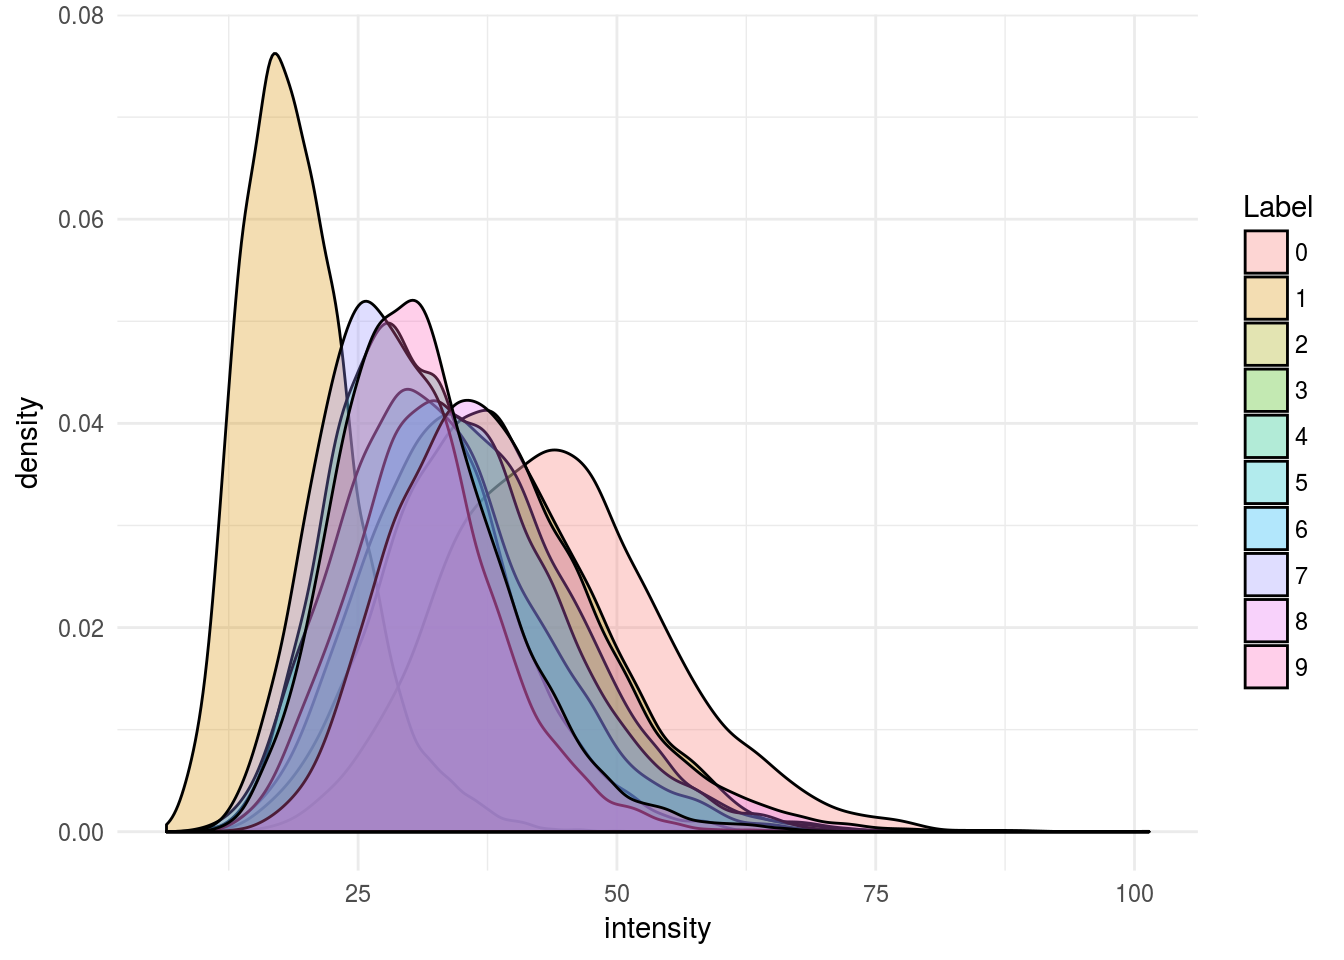
\includegraphics{mml-tutorial_files/figure-latex/density-1.pdf}

Let's try a boxplot:

\begin{Shaded}
\begin{Highlighting}[]
\KeywordTok{ggplot}\NormalTok{(mnist_df, }\KeywordTok{aes}\NormalTok{(}\DataTypeTok{x =}\NormalTok{ Label, }\DataTypeTok{y =}\NormalTok{ intensity)) }\OperatorTok{+}
\StringTok{  }\KeywordTok{geom_boxplot}\NormalTok{(}\KeywordTok{aes}\NormalTok{(}\DataTypeTok{fill =}\NormalTok{ Label), }\DataTypeTok{alpha =} \FloatTok{0.3}\NormalTok{)}
\end{Highlighting}
\end{Shaded}

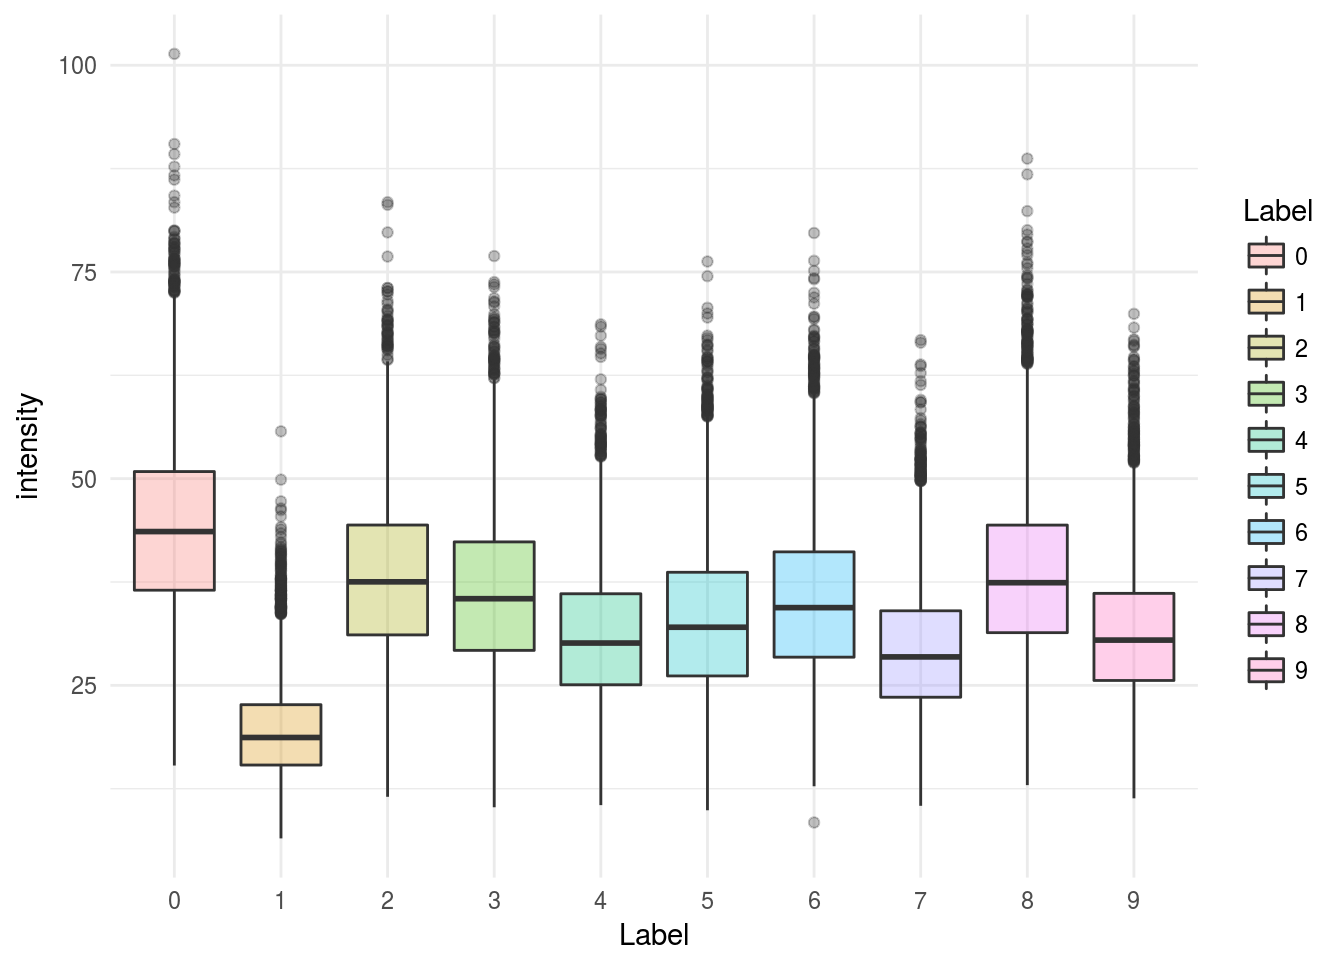
\includegraphics{mml-tutorial_files/figure-latex/boxplot-1.pdf}

\section{Visualize Digits}\label{visualize-digits}

Let's plot a sample set of digits:

\begin{Shaded}
\begin{Highlighting}[]
\NormalTok{flip <-}\StringTok{ }\ControlFlowTok{function}\NormalTok{(matrix) \{}

      \KeywordTok{apply}\NormalTok{(matrix, }\DecValTok{2}\NormalTok{, rev)}
\NormalTok{\}}

\NormalTok{plot_digit <-}\StringTok{ }\ControlFlowTok{function}\NormalTok{(samp) \{}
  
\NormalTok{  digit <-}\StringTok{ }\KeywordTok{unlist}\NormalTok{(samp)}
\NormalTok{  m <-}\StringTok{ }\KeywordTok{flip}\NormalTok{(}\KeywordTok{matrix}\NormalTok{(}\KeywordTok{rev}\NormalTok{(}\KeywordTok{as.numeric}\NormalTok{(digit)), }\DataTypeTok{nrow =} \DecValTok{28}\NormalTok{))}
  \KeywordTok{image}\NormalTok{(m, }\DataTypeTok{col =} \KeywordTok{grey.colors}\NormalTok{(}\DecValTok{255}\NormalTok{))}
  
\NormalTok{\}}

\NormalTok{mnist_df[}\DecValTok{11}\NormalTok{, ] }\OperatorTok\StringTok{ }
\StringTok{  }\KeywordTok{select}\NormalTok{(}\OperatorTok{-}\NormalTok{Label, }\OperatorTok{-}\NormalTok{intensity, }\OperatorTok{-}\NormalTok{splitVar) }\OperatorTok\StringTok{ }
\StringTok{  }\KeywordTok{sample_n}\NormalTok{(}\DecValTok{1}\NormalTok{) }\OperatorTok\StringTok{ }
\StringTok{  }\KeywordTok{rowwise}\NormalTok{() }\OperatorTok\StringTok{ }\NormalTok{plot_digit}
\end{Highlighting}
\end{Shaded}

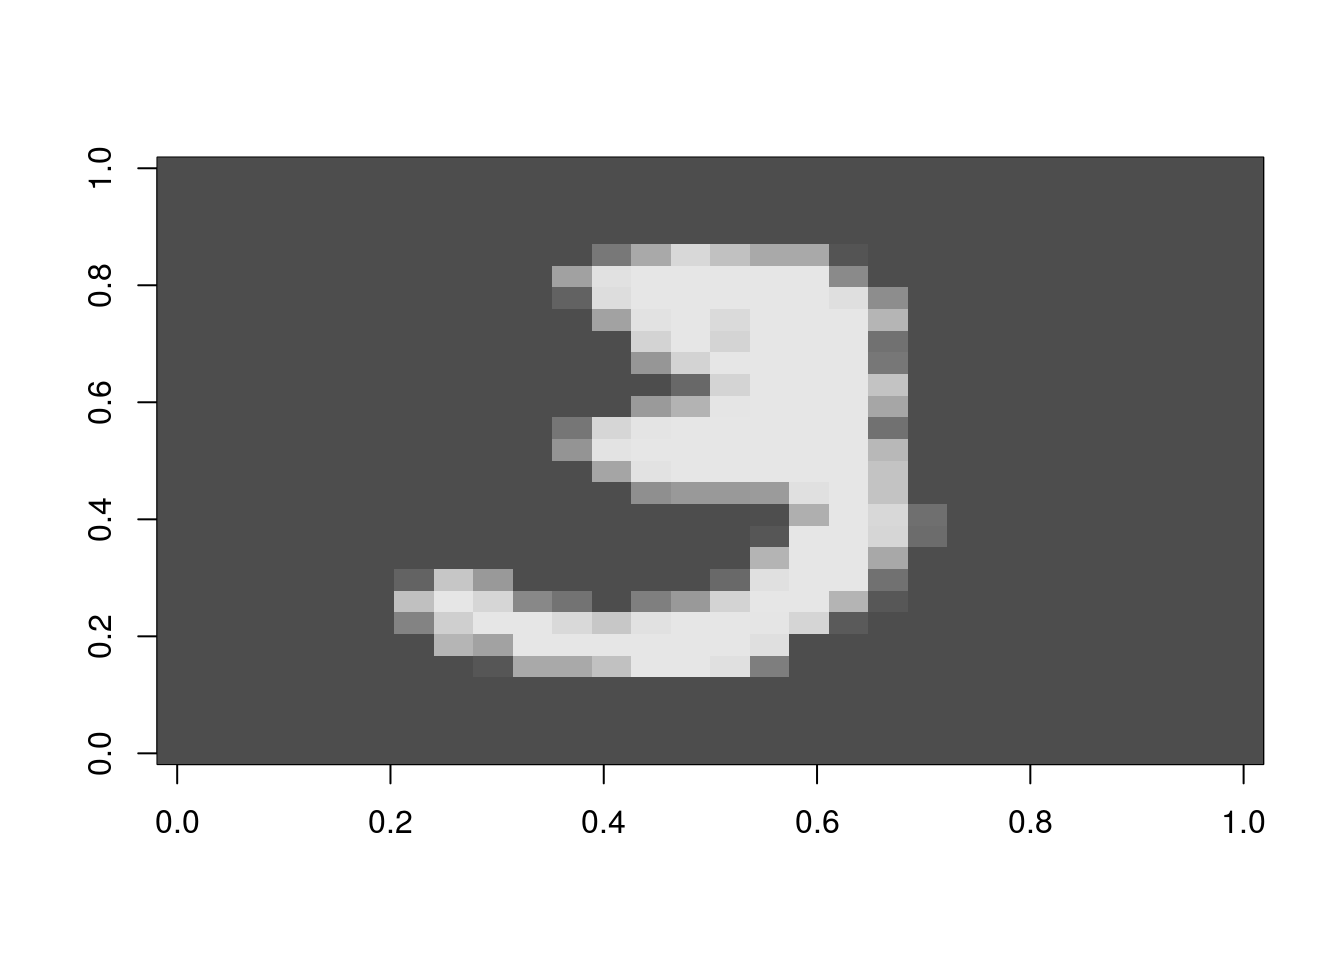
\includegraphics{mml-tutorial_files/figure-latex/displayimage-1.pdf}

\section{Split the Data into Train and Test
Sets}\label{split-the-data-into-train-and-test-sets}

\begin{Shaded}
\begin{Highlighting}[]
\NormalTok{splits <-}\StringTok{ }\KeywordTok{rxSplit}\NormalTok{(mnist_xdf,}
                  \DataTypeTok{splitByFactor =} \StringTok{"splitVar"}\NormalTok{, }
                  \DataTypeTok{overwrite =} \OtherTok{TRUE}\NormalTok{)}
\KeywordTok{names}\NormalTok{(splits) <-}\StringTok{ }\KeywordTok{c}\NormalTok{(}\StringTok{"train"}\NormalTok{, }\StringTok{"test"}\NormalTok{)}
\end{Highlighting}
\end{Shaded}

Let's first train a softmax classifier using the
\texttt{rxLogisticRegression}:

\begin{Shaded}
\begin{Highlighting}[]
\NormalTok{softmax <-}\StringTok{ }\KeywordTok{estimate_model}\NormalTok{(}\DataTypeTok{xdf_data =}\NormalTok{ splits}\OperatorTok{$}\NormalTok{train,}
                          \DataTypeTok{form =} \KeywordTok{make_form}\NormalTok{(splits}\OperatorTok{$}\NormalTok{train, }
                                           \DataTypeTok{resp_var =} \StringTok{"Label"}\NormalTok{, }
                                           \DataTypeTok{vars_to_skip =} \KeywordTok{c}\NormalTok{(}\StringTok{"splitVar"}\NormalTok{)),}
                          \DataTypeTok{model =}\NormalTok{ rxLogisticRegression,}
                          \DataTypeTok{type =} \StringTok{"multiClass"}\NormalTok{)}
\end{Highlighting}
\end{Shaded}

\begin{verbatim}
## Automatically adding a MinMax normalization transform, use 'norm=Warn' or 'norm=No' to turn this behavior off.
## LBFGS multi-threading will attempt to load dataset into memory. In case of out-of-memory issues, turn off multi-threading by setting trainThreads to 1.
## Beginning optimization
## num vars: 7850
## improvement criterion: Mean Improvement
## L1 regularization selected 3699 of 7850 weights.
## Not training a calibrator because it is not needed.
## Elapsed time: 00:00:17.3789513
## Elapsed time: 00:00:00.0199858
\end{verbatim}

Let's see how we did. Let's examine our results on the train set:

\begin{Shaded}
\begin{Highlighting}[]
\NormalTok{softmax_scores <-}\StringTok{ }\KeywordTok{rxPredict}\NormalTok{(}\DataTypeTok{modelObject =}\NormalTok{ softmax, }
                            \DataTypeTok{data =}\NormalTok{ splits}\OperatorTok{$}\NormalTok{test, }
                            \DataTypeTok{outData =} \KeywordTok{tempfile}\NormalTok{(}\DataTypeTok{fileext =} \StringTok{".xdf"}\NormalTok{),}
                            \DataTypeTok{overwrite =} \OtherTok{TRUE}\NormalTok{,}
                            \DataTypeTok{extraVarsToWrite =} \StringTok{"Label"}\NormalTok{)}
\end{Highlighting}
\end{Shaded}

\begin{verbatim}
## Elapsed time: 00:00:00.9645786
\end{verbatim}

We can make a confusion matrix of all our results:

\begin{Shaded}
\begin{Highlighting}[]
\KeywordTok{rxCube}\NormalTok{( }\OperatorTok{~}\StringTok{ }\NormalTok{Label }\OperatorTok{:}\StringTok{ }\NormalTok{PredictedLabel , }\DataTypeTok{data =}\NormalTok{ softmax_scores,}
       \DataTypeTok{returnDataFrame =} \OtherTok{TRUE}\NormalTok{) ->}\StringTok{ }\NormalTok{softmax_scores_df}

\NormalTok{softmax_scores_df }\OperatorTok\StringTok{ }\KeywordTok{ggplot}\NormalTok{(}\KeywordTok{aes}\NormalTok{(}\DataTypeTok{x =}\NormalTok{ Label, }\DataTypeTok{y =}\NormalTok{ PredictedLabel,}
                                 \DataTypeTok{fill =}\NormalTok{ Counts)) }\OperatorTok{+}
\StringTok{  }\KeywordTok{geom_raster}\NormalTok{() }\OperatorTok{+}
\StringTok{  }\KeywordTok{scale_fill_continuous}\NormalTok{(}\DataTypeTok{low =} \StringTok{"steelblue2"}\NormalTok{, }\DataTypeTok{high =} \StringTok{"mediumblue"}\NormalTok{)}
\end{Highlighting}
\end{Shaded}

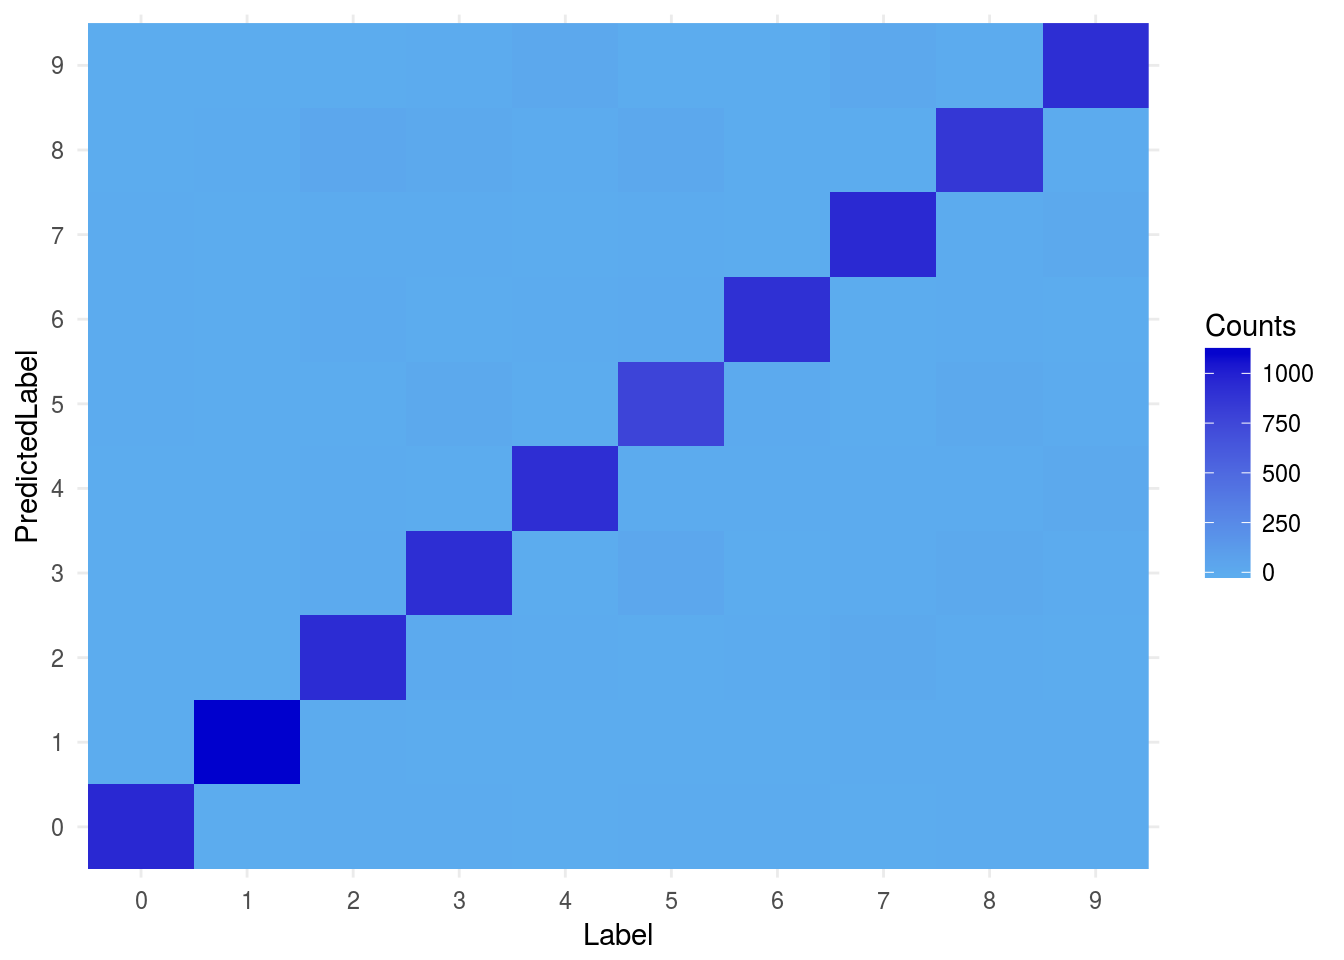
\includegraphics{mml-tutorial_files/figure-latex/conf_softmax-1.pdf}

Here we are plotting the raw counts. This might unfairly represent the
more populated classes. Let's weight each count by the total number of
samples in that class:

\begin{Shaded}
\begin{Highlighting}[]
\NormalTok{label_rates <-}\StringTok{ }\NormalTok{softmax_scores_df }\OperatorTok\StringTok{ }
\StringTok{  }\NormalTok{tbl_df }\OperatorTok\StringTok{ }
\StringTok{  }\KeywordTok{group_by}\NormalTok{(Label) }\OperatorTok\StringTok{ }
\StringTok{  }\KeywordTok{mutate}\NormalTok{(}\DataTypeTok{rate =}\NormalTok{ Counts}\OperatorTok{/}\KeywordTok{sum}\NormalTok{(Counts))}

\NormalTok{label_rates }\OperatorTok\StringTok{ }\KeywordTok{ggplot}\NormalTok{(}\KeywordTok{aes}\NormalTok{(}\DataTypeTok{x =}\NormalTok{ Label, }\DataTypeTok{y =}\NormalTok{ PredictedLabel, }\DataTypeTok{fill =}\NormalTok{ rate)) }\OperatorTok{+}
\StringTok{  }\KeywordTok{geom_raster}\NormalTok{() }\OperatorTok{+}
\StringTok{  }\KeywordTok{scale_fill_continuous}\NormalTok{(}\DataTypeTok{low =} \StringTok{"steelblue2"}\NormalTok{, }\DataTypeTok{high =} \StringTok{"mediumblue"}\NormalTok{)}
\end{Highlighting}
\end{Shaded}

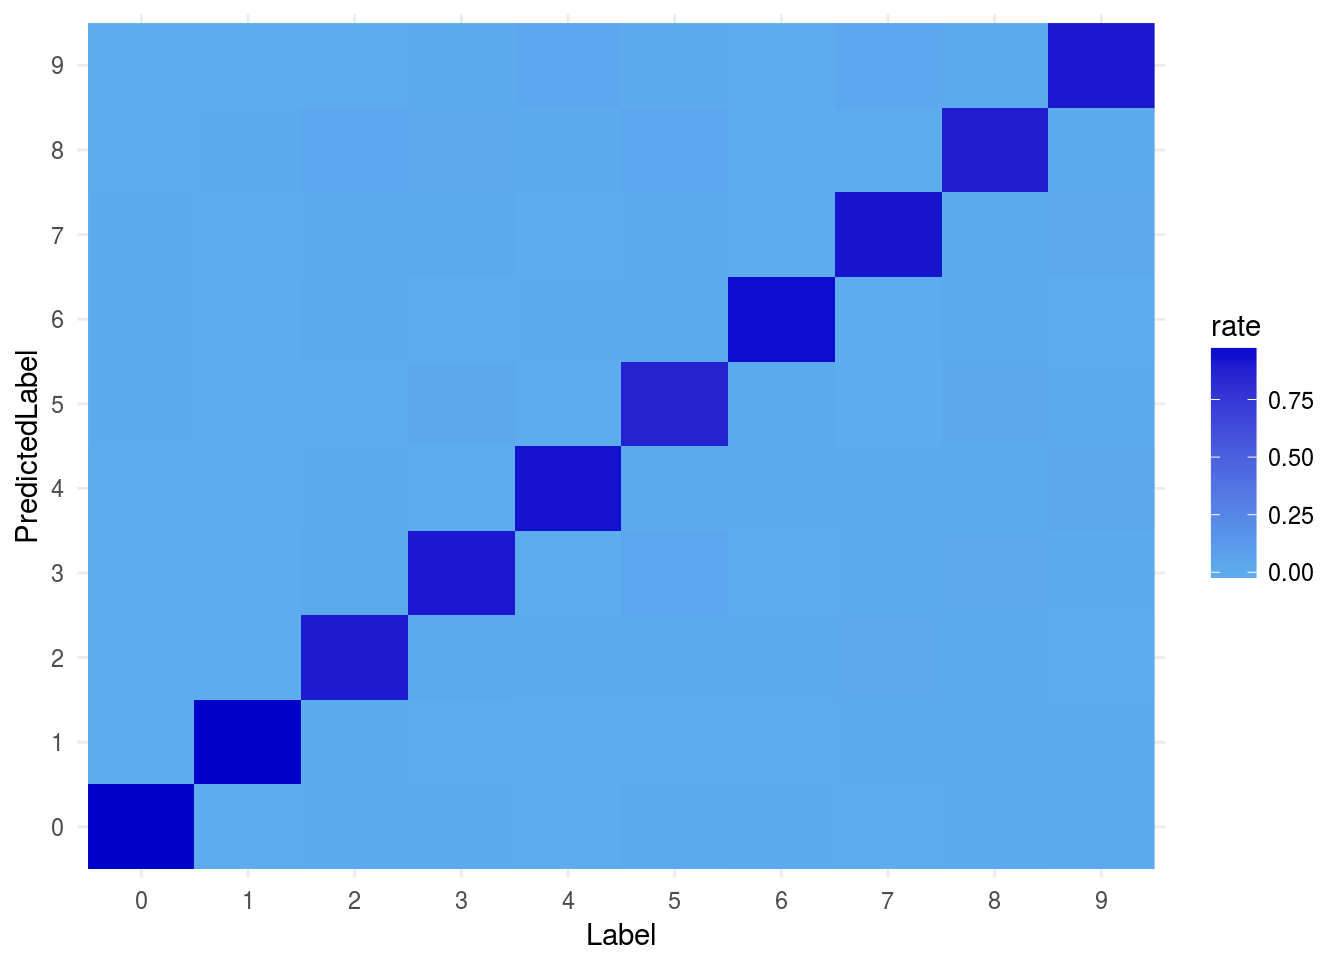
\includegraphics{mml-tutorial_files/figure-latex/rates-1.pdf}

Let's fill out all the correct scores with zeros so we can see the
errors more clearly:

\begin{Shaded}
\begin{Highlighting}[]
\NormalTok{label_rates }\OperatorTok
\StringTok{  }\KeywordTok{mutate}\NormalTok{(}\DataTypeTok{error_rate =} \KeywordTok{ifelse}\NormalTok{(Label }\OperatorTok{==}\StringTok{ }\NormalTok{PredictedLabel,}
                             \DecValTok{0}\NormalTok{, rate)) }\OperatorTok\StringTok{ }
\StringTok{  }\KeywordTok{ggplot}\NormalTok{(}\KeywordTok{aes}\NormalTok{(}\DataTypeTok{x =}\NormalTok{ Label, }\DataTypeTok{y =}\NormalTok{ PredictedLabel, }\DataTypeTok{fill =}\NormalTok{ error_rate)) }\OperatorTok{+}
\StringTok{  }\KeywordTok{geom_raster}\NormalTok{() }\OperatorTok{+}
\StringTok{  }\KeywordTok{scale_fill_continuous}\NormalTok{(}\DataTypeTok{low =} \StringTok{"steelblue2"}\NormalTok{, }\DataTypeTok{high =} \StringTok{"mediumblue"}\NormalTok{,}
                        \DataTypeTok{labels =}\NormalTok{ scales}\OperatorTok{::}\NormalTok{percent)}
\end{Highlighting}
\end{Shaded}

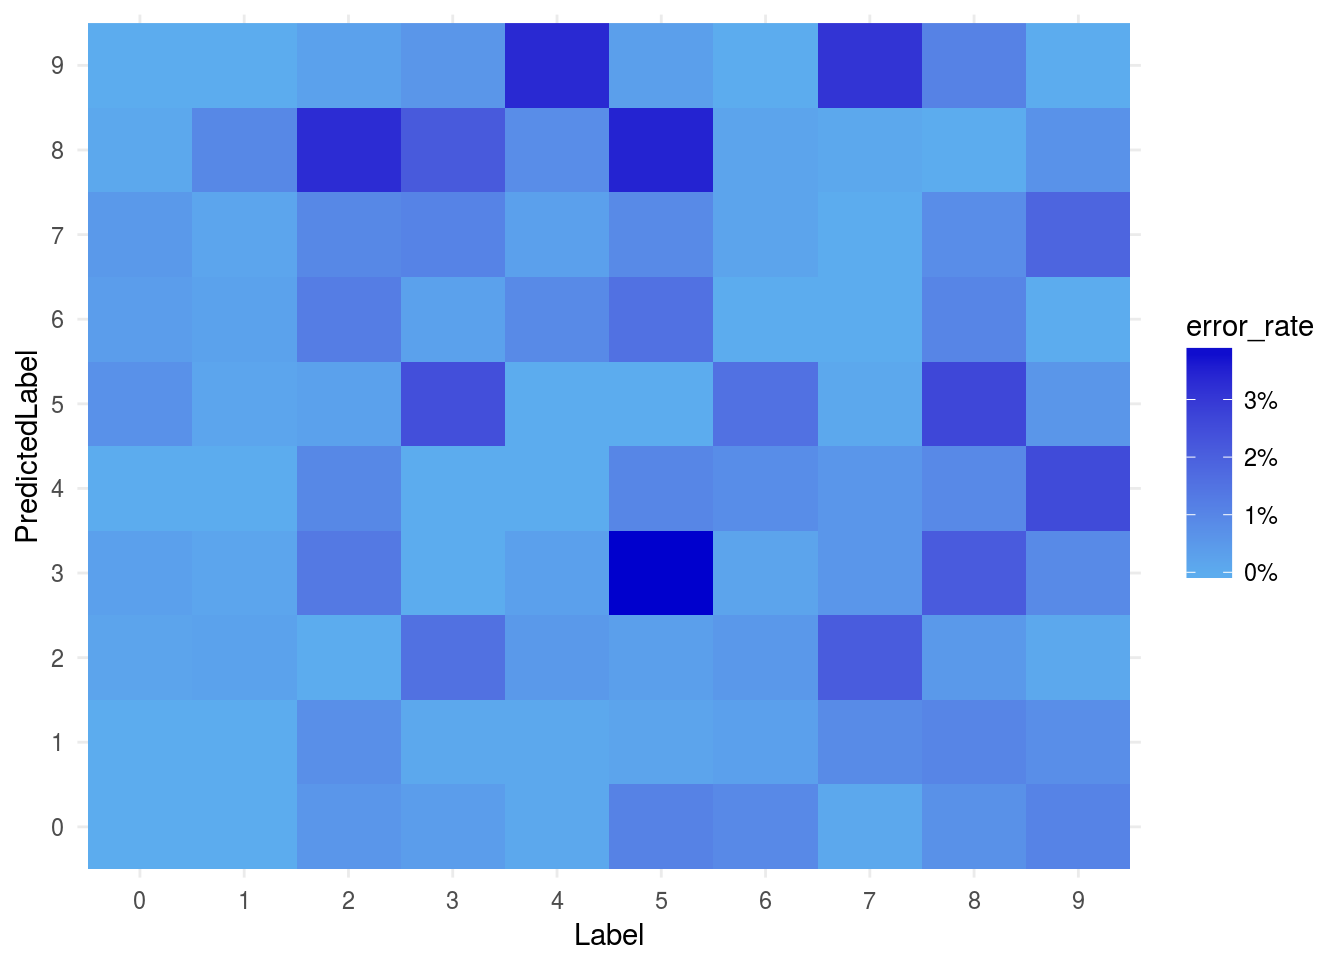
\includegraphics{mml-tutorial_files/figure-latex/errors-1.pdf}

\section{Exercises}\label{exercises-1}

\begin{enumerate}
\def\labelenumi{\arabic{enumi}.}
\tightlist
\item
  Take a look at David Robinson's
  \href{https://twitter.com/drob/status/869991240099549185}{tweet} on
  using a single pixel to distinguish between pairs of digits.
\item
  You can find his
  \href{https://gist.github.com/dgrtwo/aaef94ecc6a60cd50322c0054cc04478}{gist}
  saved in the \href{../Rscripts/8-drob-just-a-pixel.R}{Rscripts
  directory}.
\end{enumerate}

\chapter{Convolutional Neural Networks for Computer
Vision}\label{convolutional-neural-networks-for-computer-vision}

In the previous section we conducted multi-class classification using a
softmax regression algorithm. The most popular approach for image
classification is now convolutional neural networks. This module
describes how to use convolutional networks.

MicrosoftML uses the
\href{https://docs.microsoft.com/en-us/azure/machine-learning/machine-learning-azure-ml-netsharp-reference-guide}{Net\#}
specification for defining neural network architectures. In the
\texttt{../nnet} directory, we have already created the specifications
for you.

Examine the architecture in ``MNIST.nn''. In this network, we have two
convolutional layers and one fully connected layer.

\begin{Shaded}
\begin{Highlighting}[]
\KeywordTok{library}\NormalTok{(tidyverse)}
\KeywordTok{library}\NormalTok{(MicrosoftML)}
\KeywordTok{theme_set}\NormalTok{(}\KeywordTok{theme_minimal}\NormalTok{())}

\NormalTok{rxNeuralNetFile <-}\StringTok{ }\KeywordTok{file.path}\NormalTok{(}\StringTok{"nnet/MNIST.nn"}\NormalTok{)}
\NormalTok{nn <-}\StringTok{ }\KeywordTok{readChar}\NormalTok{(rxNeuralNetFile, }\KeywordTok{file.info}\NormalTok{(rxNeuralNetFile)}\OperatorTok{$}\NormalTok{size)}
\NormalTok{nnet_fit <-}\StringTok{ }\KeywordTok{rxNeuralNet}\NormalTok{(}\KeywordTok{make_form}\NormalTok{(splits}\OperatorTok{$}\NormalTok{train,}
                                  \DataTypeTok{resp_var =} \StringTok{"Label"}\NormalTok{,}
                                  \DataTypeTok{vars_to_skip =} \KeywordTok{c}\NormalTok{(}\StringTok{"splitVar"}\NormalTok{)),}
                              \DataTypeTok{data =}\NormalTok{ splits}\OperatorTok{$}\NormalTok{train,}
                              \DataTypeTok{type =} \StringTok{"multiClass"}\NormalTok{,}
                              \DataTypeTok{numIterations =} \DecValTok{9}\NormalTok{,}
                              \DataTypeTok{netDefinition =}\NormalTok{ nn,}
                              \DataTypeTok{initWtsDiameter =} \FloatTok{1.0}\NormalTok{,}
                              \DataTypeTok{normalize =} \StringTok{"No"}\NormalTok{)}
\end{Highlighting}
\end{Shaded}

\begin{verbatim}
## Not adding a normalizer.
## Using: SSE Math
## Loading net from: 
## ***** Net definition *****
##   const T = true;
##   const F = false;
##   input Picture [28, 28];
##   hidden Convolve1 [5, 12, 12] from Picture convolve {
##     InputShape = [28, 28];
##     KernelShape = [5, 5];
##     Stride = [2, 2];
##     MapCount = 5;
##   }
##   hidden Convolve2 [50, 4, 4] from Convolve1 convolve {
##     InputShape = [5, 12, 12];
##     KernelShape = [1, 5, 5];
##     Stride = [1, 2, 2];
##     Sharing = [F, T, T];
##     MapCount = 10;
##   }
##   hidden Full3 [100] from Convolve2 all;
##   output Result [10] from Full3 all;
## ***** Reduced *****
##   const T = true;
##   const F = false;
##   input Picture [28, 28];
##   hidden Convolve1 [5, 12, 12] from Picture convolve {
##     InputShape = [28, 28];
##     KernelShape = [5, 5];
##     Stride = [2, 2];
##     MapCount = 5;
##   }
##   hidden Convolve2 [50, 4, 4] from Convolve1 convolve {
##     InputShape = [5, 12, 12];
##     KernelShape = [1, 5, 5];
##     Stride = [1, 2, 2];
##     Sharing = [false, true, true];
##     MapCount = 10;
##   }
##   hidden Full3 100 from Convolve2 all;
##   output Result 10 from Full3 all;
## ***** End net definition *****
## Input count: 784
## Output count: 10
## Output Function: SoftMax
## Loss Function: CrossEntropy
## PreTrainer: NoPreTrainer
## ___________________________________________________________________
## Starting training...
## Learning rate: 0.001000
## Momentum: 0.000000
## InitWtsDiameter: 1.000000
## ___________________________________________________________________
## Initializing 3 Hidden Layers, 82540 Weights...
## Estimated Pre-training MeanError = 4.142561
## Iter:1/9, MeanErr=1.582342(-61.80%), 590.01M WeightUpdates/sec
## Iter:2/9, MeanErr=0.651257(-58.84%), 598.09M WeightUpdates/sec
## Iter:3/9, MeanErr=0.474688(-27.11%), 603.13M WeightUpdates/sec
## Iter:4/9, MeanErr=0.390425(-17.75%), 616.42M WeightUpdates/sec
## Iter:5/9, MeanErr=0.344977(-11.64%), 595.88M WeightUpdates/sec
## Iter:6/9, MeanErr=0.314282(-8.90%), 606.88M WeightUpdates/sec
## Iter:7/9, MeanErr=0.290820(-7.47%), 609.71M WeightUpdates/sec
## Iter:8/9, MeanErr=0.273693(-5.89%), 609.05M WeightUpdates/sec
## Iter:9/9, MeanErr=0.256158(-6.41%), 631.54M WeightUpdates/sec
## Done!
## Estimated Post-training MeanError = 0.247149
## ___________________________________________________________________
## Not training a calibrator because it is not needed.
## Elapsed time: 00:01:25.7559992
\end{verbatim}

As in the previous section with linear classifiers, we can create our
confusion matrices:

\begin{Shaded}
\begin{Highlighting}[]
\NormalTok{nnet_score <-}\StringTok{ }\KeywordTok{rxPredict}\NormalTok{(}\DataTypeTok{modelObject =}\NormalTok{ nnet_fit,}
                        \DataTypeTok{data =}\NormalTok{ splits}\OperatorTok{$}\NormalTok{test,}
                        \DataTypeTok{outData =} \KeywordTok{tempfile}\NormalTok{(}\DataTypeTok{fileext =} \StringTok{".xdf"}\NormalTok{),}
                        \DataTypeTok{overwrite =} \OtherTok{TRUE}\NormalTok{,}
                        \DataTypeTok{extraVarsToWrite =} \StringTok{"Label"}\NormalTok{)}
\end{Highlighting}
\end{Shaded}

\begin{verbatim}
## Elapsed time: 00:00:01.3485847
\end{verbatim}

Now that we have our scored results, let's put them in a confusion
matrix:

\begin{Shaded}
\begin{Highlighting}[]
\KeywordTok{rxCube}\NormalTok{( }\OperatorTok{~}\StringTok{ }\NormalTok{Label }\OperatorTok{:}\StringTok{ }\NormalTok{PredictedLabel , }\DataTypeTok{data =}\NormalTok{ nnet_score,}
       \DataTypeTok{returnDataFrame =} \OtherTok{TRUE}\NormalTok{) ->}\StringTok{ }\NormalTok{nnet_scores_df}

\NormalTok{nnet_scores_df }\OperatorTok\StringTok{ }
\StringTok{  }\NormalTok{tbl_df }\OperatorTok\StringTok{ }
\StringTok{  }\KeywordTok{group_by}\NormalTok{(Label) }\OperatorTok\StringTok{ }
\StringTok{  }\KeywordTok{mutate}\NormalTok{(}\DataTypeTok{rate =}\NormalTok{ Counts}\OperatorTok{/}\KeywordTok{sum}\NormalTok{(Counts)) }\OperatorTok
\StringTok{  }\KeywordTok{mutate}\NormalTok{(}\DataTypeTok{error_rate =} \KeywordTok{ifelse}\NormalTok{(Label }\OperatorTok{==}\StringTok{ }\NormalTok{PredictedLabel,}
                             \DecValTok{0}\NormalTok{, rate)) }\OperatorTok\StringTok{ }
\StringTok{  }\KeywordTok{ggplot}\NormalTok{(}\KeywordTok{aes}\NormalTok{(}\DataTypeTok{x =}\NormalTok{ Label, }\DataTypeTok{y =}\NormalTok{ PredictedLabel, }\DataTypeTok{fill =}\NormalTok{ error_rate)) }\OperatorTok{+}
\StringTok{  }\KeywordTok{geom_raster}\NormalTok{() }\OperatorTok{+}
\StringTok{  }\KeywordTok{scale_fill_continuous}\NormalTok{(}\DataTypeTok{low =} \StringTok{"steelblue2"}\NormalTok{, }\DataTypeTok{high =} \StringTok{"mediumblue"}\NormalTok{,}
                        \DataTypeTok{labels =}\NormalTok{ scales}\OperatorTok{::}\NormalTok{percent)}
\end{Highlighting}
\end{Shaded}

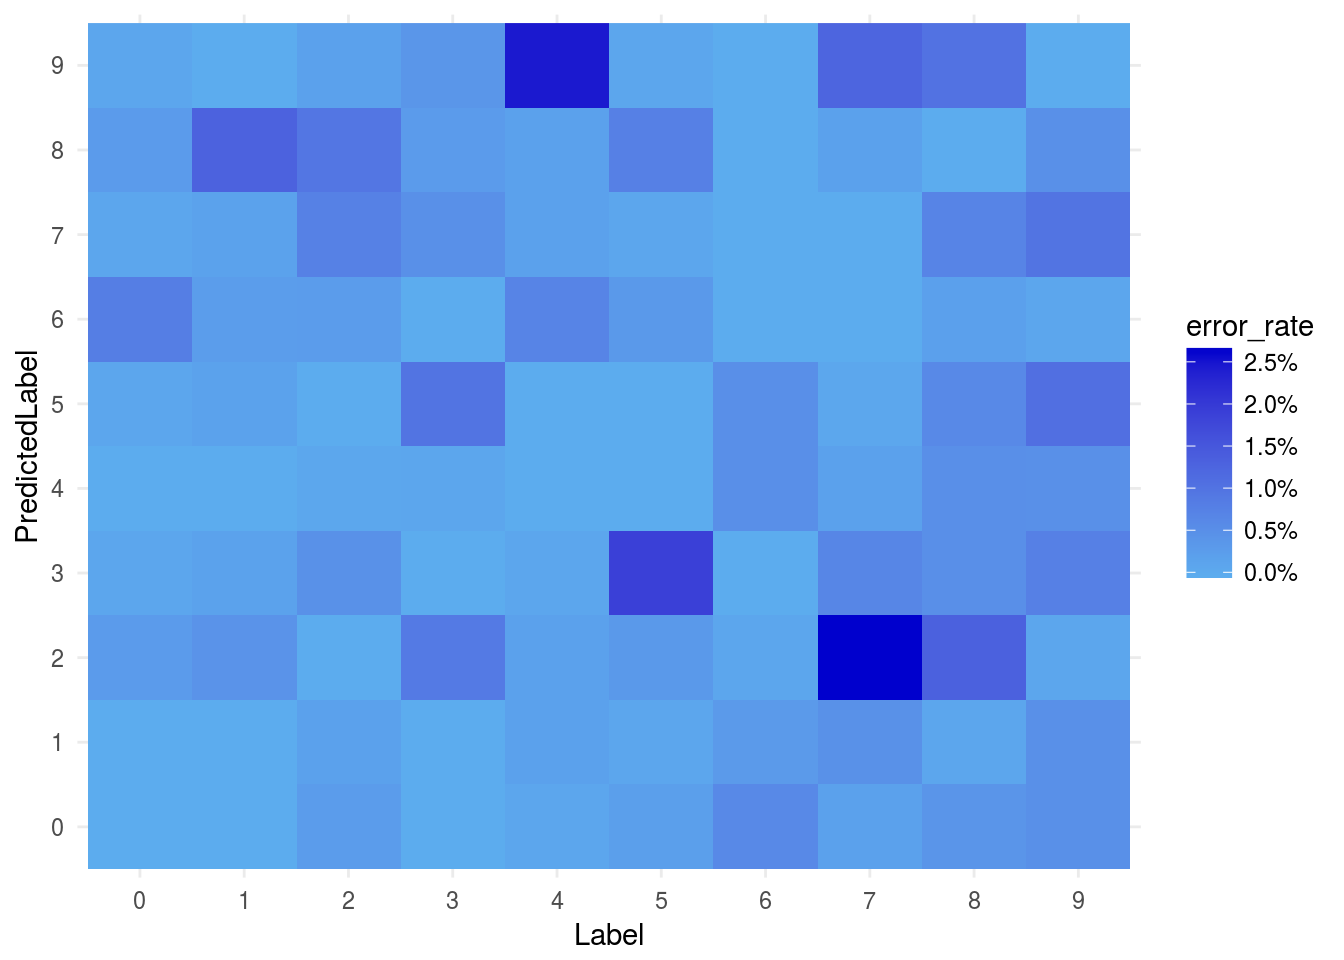
\includegraphics{mml-tutorial_files/figure-latex/nnet_confusion-1.pdf}

Just judging from the label it looks we have already done better than
the linear classifier.

\section{LeNet-5}\label{lenet-5}

Convolutional neural networks were popularized by Yann LeCun. In this
section, we'll fit his model from 1998, effectionately called
\href{http://yann.lecun.com/exdb/publis/pdf/lecun-98.pdf}{LeNet-5}.

The network differs from the previous implementation in that there are
now more layers, but in between layers there is a pooling/sampling
layer. This helps preventing the neural network from overfitting in
between layers and allows for extracting higher-order representations
from the data.

Because this neural network has significantly more weights to learn,
it'll take a while longer, especially if we aren't using GPUs (which
would give us at least 5-7x speed improvement). If you're especially
impatient, you can lower the \texttt{numIterations} parameter.

\begin{Shaded}
\begin{Highlighting}[]
\NormalTok{rxNeuralNetFile <-}\StringTok{ }\KeywordTok{file.path}\NormalTok{(}\StringTok{"nnet/LeCun5.nn"}\NormalTok{)}
\NormalTok{lecun <-}\StringTok{ }\KeywordTok{readChar}\NormalTok{(rxNeuralNetFile, }\KeywordTok{file.info}\NormalTok{(rxNeuralNetFile)}\OperatorTok{$}\NormalTok{size)}
\KeywordTok{system.time}\NormalTok{(lenet_fit <-}\StringTok{ }\KeywordTok{rxNeuralNet}\NormalTok{(}\KeywordTok{make_form}\NormalTok{(splits}\OperatorTok{$}\NormalTok{train,}
                                               \DataTypeTok{resp_var =} \StringTok{"Label"}\NormalTok{,}
                                               \DataTypeTok{vars_to_skip =} \KeywordTok{c}\NormalTok{(}\StringTok{"splitVar"}\NormalTok{)),}
                                     \DataTypeTok{data =}\NormalTok{ splits}\OperatorTok{$}\NormalTok{train,}
                                     \DataTypeTok{type =} \StringTok{"multiClass"}\NormalTok{,}
                                     \DataTypeTok{numIterations =} \DecValTok{9}\NormalTok{,}
                                     \DataTypeTok{netDefinition =}\NormalTok{ lecun,}
                                     \DataTypeTok{initWtsDiameter =} \FloatTok{1.0}\NormalTok{,}
                                     \DataTypeTok{normalize =} \StringTok{"No"}\NormalTok{))}
\end{Highlighting}
\end{Shaded}

\begin{verbatim}
## Not adding a normalizer.
## Using: SSE Math
## Loading net from: 
## ***** Net definition *****
##   const T = true;
##   const F = false;
##   input Picture [28, 28];
##   hidden Convolve1 [6, 28, 28] from Picture convolve {
##     Padding = T;
##     InputShape = [28, 28];
##     KernelShape = [5, 5];
##     MapCount = 6;
##   }
##   hidden Subsample2 [6, 14, 14] linear from Convolve1 convolve {
##     InputShape = [6, 28, 28];
##     KernelShape = [1, 2, 2];
##     Stride = [1, 2, 2];
##     Sharing = [F, T, T];
##   }
##   hidden Convolve3 [16, 10, 10] from Subsample2 convolve {
##     InputShape = [6, 14, 14];
##     KernelShape = [6, 5, 5];
##     MapCount = 16;
##   }
##   hidden Subsample4 [16, 5, 5] linear from Convolve3 convolve {
##     InputShape = [16, 10, 10];
##     KernelShape = [1, 2, 2];
##     Stride = [1, 2, 2];
##     Sharing = [F, T, T];
##   }
##   hidden Convolve5 [120] from Subsample4 convolve {
##     InputShape = [16, 5, 5];
##     KernelShape = [16, 5, 5];
##     MapCount = 120;
##   }
##   hidden Full6 [84] from Convolve5 all;
##   output Result [10] softmax from Full6 all;
## ***** Reduced *****
##   const T = true;
##   const F = false;
##   input Picture [28, 28];
##   hidden Convolve1 [6, 28, 28] from Picture convolve {
##     Padding = true;
##     InputShape = [28, 28];
##     KernelShape = [5, 5];
##     MapCount = 6;
##   }
##   hidden Subsample2 [6, 14, 14] linear from Convolve1 convolve {
##     InputShape = [6, 28, 28];
##     KernelShape = [1, 2, 2];
##     Stride = [1, 2, 2];
##     Sharing = [false, true, true];
##   }
##   hidden Convolve3 [16, 10, 10] from Subsample2 convolve {
##     InputShape = [6, 14, 14];
##     KernelShape = [6, 5, 5];
##     MapCount = 16;
##   }
##   hidden Subsample4 [16, 5, 5] linear from Convolve3 convolve {
##     InputShape = [16, 10, 10];
##     KernelShape = [1, 2, 2];
##     Stride = [1, 2, 2];
##     Sharing = [false, true, true];
##   }
##   hidden Convolve5 120 from Subsample4 convolve {
##     InputShape = [16, 5, 5];
##     KernelShape = [16, 5, 5];
##     MapCount = 120;
##   }
##   hidden Full6 84 from Convolve5 all;
##   output Result 10 softmax from Full6 all;
## ***** End net definition *****
## Input count: 784
## Output count: 10
## Output Function: SoftMax
## Loss Function: CrossEntropy
## PreTrainer: NoPreTrainer
## ___________________________________________________________________
## Starting training...
## Learning rate: 0.001000
## Momentum: 0.000000
## InitWtsDiameter: 1.000000
## ___________________________________________________________________
## Initializing 6 Hidden Layers, 61816 Weights...
## Estimated Pre-training MeanError = 4.016721
## Iter:1/9, MeanErr=1.566115(-61.01%), 78.16M WeightUpdates/sec
## Iter:2/9, MeanErr=0.508592(-67.53%), 80.91M WeightUpdates/sec
## Iter:3/9, MeanErr=0.350416(-31.10%), 81.29M WeightUpdates/sec
## Iter:4/9, MeanErr=0.274144(-21.77%), 81.72M WeightUpdates/sec
## Iter:5/9, MeanErr=0.231398(-15.59%), 80.61M WeightUpdates/sec
## Iter:6/9, MeanErr=0.200124(-13.52%), 80.79M WeightUpdates/sec
## Iter:7/9, MeanErr=0.180827(-9.64%), 80.66M WeightUpdates/sec
## Iter:8/9, MeanErr=0.165253(-8.61%), 80.67M WeightUpdates/sec
## Iter:9/9, MeanErr=0.154163(-6.71%), 80.19M WeightUpdates/sec
## Done!
## Estimated Post-training MeanError = 0.140622
## ___________________________________________________________________
## Not training a calibrator because it is not needed.
## Elapsed time: 00:07:32.4435112
\end{verbatim}

\begin{verbatim}
##    user  system elapsed 
##    0.04    0.00  452.57
\end{verbatim}

As before, let's score our pretty model:

\begin{Shaded}
\begin{Highlighting}[]
\NormalTok{lescores <-}\StringTok{ }\KeywordTok{rxPredict}\NormalTok{(}\DataTypeTok{modelObject =}\NormalTok{ lenet_fit,}
                      \DataTypeTok{data =}\NormalTok{ splits}\OperatorTok{$}\NormalTok{test,}
                      \DataTypeTok{outData =} \KeywordTok{tempfile}\NormalTok{(}\DataTypeTok{fileext =} \StringTok{".xdf"}\NormalTok{),}
                      \DataTypeTok{overwrite =} \OtherTok{TRUE}\NormalTok{,}
                      \DataTypeTok{extraVarsToWrite =} \StringTok{"Label"}\NormalTok{)}
\end{Highlighting}
\end{Shaded}

\begin{verbatim}
## Elapsed time: 00:00:03.4389931
\end{verbatim}

and visualize our error rates:

\begin{Shaded}
\begin{Highlighting}[]
\KeywordTok{rxCube}\NormalTok{( }\OperatorTok{~}\StringTok{ }\NormalTok{Label }\OperatorTok{:}\StringTok{ }\NormalTok{PredictedLabel , }\DataTypeTok{data =}\NormalTok{ lescores,}
       \DataTypeTok{returnDataFrame =} \OtherTok{TRUE}\NormalTok{) ->}\StringTok{ }\NormalTok{le_scores_df}

\NormalTok{le_scores_df }\OperatorTok\StringTok{ }
\StringTok{  }\NormalTok{tbl_df }\OperatorTok\StringTok{ }
\StringTok{  }\KeywordTok{group_by}\NormalTok{(Label) }\OperatorTok\StringTok{ }
\StringTok{  }\KeywordTok{mutate}\NormalTok{(}\DataTypeTok{rate =}\NormalTok{ Counts}\OperatorTok{/}\KeywordTok{sum}\NormalTok{(Counts)) }\OperatorTok
\StringTok{  }\KeywordTok{mutate}\NormalTok{(}\DataTypeTok{error_rate =} \KeywordTok{ifelse}\NormalTok{(Label }\OperatorTok{==}\StringTok{ }\NormalTok{PredictedLabel,}
                             \DecValTok{0}\NormalTok{, rate)) }\OperatorTok\StringTok{ }
\StringTok{  }\KeywordTok{ggplot}\NormalTok{(}\KeywordTok{aes}\NormalTok{(}\DataTypeTok{x =}\NormalTok{ Label, }\DataTypeTok{y =}\NormalTok{ PredictedLabel, }\DataTypeTok{fill =}\NormalTok{ error_rate)) }\OperatorTok{+}
\StringTok{  }\KeywordTok{geom_raster}\NormalTok{() }\OperatorTok{+}
\StringTok{  }\KeywordTok{scale_fill_continuous}\NormalTok{(}\DataTypeTok{low =} \StringTok{"steelblue2"}\NormalTok{, }\DataTypeTok{high =} \StringTok{"mediumblue"}\NormalTok{,}
                        \DataTypeTok{labels =}\NormalTok{ scales}\OperatorTok{::}\NormalTok{percent)}
\end{Highlighting}
\end{Shaded}

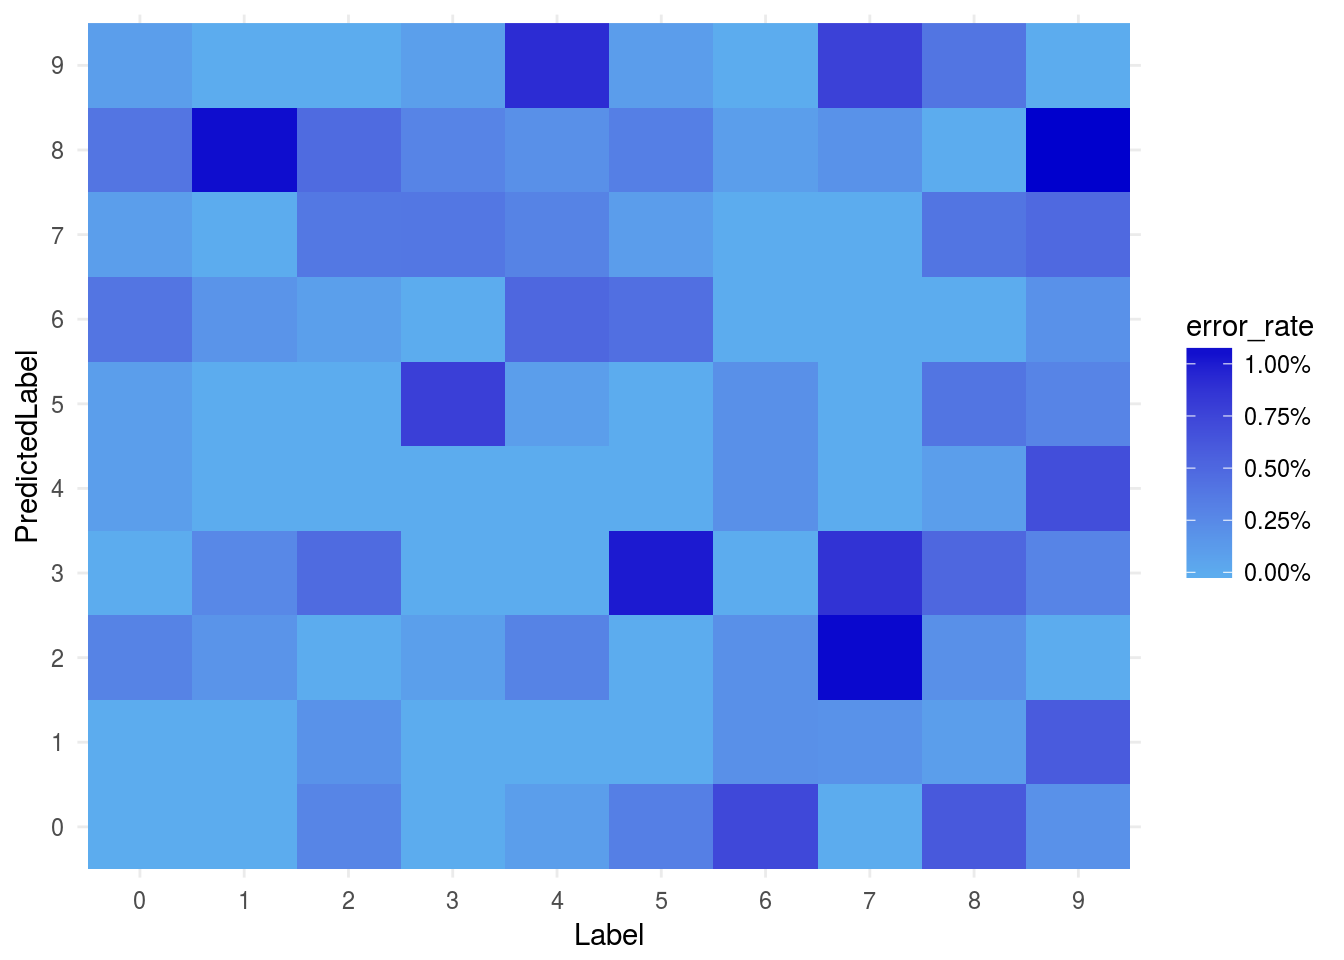
\includegraphics{mml-tutorial_files/figure-latex/leconfusion-1.pdf}

Looks even better!

\section{Model Metrics}\label{model-metrics}

While our visualizations provide some insight into our model's
improvement, let's try to calculate empricial metrics of our models'
performacne.

The three metrics we'll focus on are ``accuracy'', ``precision'', and
``recall''. Accuracy simply measures how many of our estimates we
classified correctly. While simple and intuitive, it does not account
for class-imbalances. For example, if 99\% of our data is in class A,
and we simply use the rule that everything is class A, we'll get an
accuracy of 99\%. Sounds impressive, but probably not going to win any
Turing tests.

\subsection{Accuracy}\label{accuracy}

To calculate accuracy, we can simply measure the sum of our confusion
matrix's diagonal over all values. Our data was in a long format to make
it amenable for visualizations using ggplot2. Here we'll use
\texttt{tidyr} to put it into a wide format amenable for calculating
model metrics quickly and efficiently.

\begin{Shaded}
\begin{Highlighting}[]
\NormalTok{calc_accuracy <-}\StringTok{ }\ControlFlowTok{function}\NormalTok{(scores_df) \{}
  
  \KeywordTok{library}\NormalTok{(tidyr)}
  
\NormalTok{  scores_df <-}\StringTok{ }\KeywordTok{as.data.frame}\NormalTok{(scores_df)}
\NormalTok{  scores_conf <-}\StringTok{ }\NormalTok{scores_df }\OperatorTok\StringTok{ }\KeywordTok{spread}\NormalTok{(PredictedLabel, Counts)}
  
\NormalTok{  scores_conf <-}\StringTok{ }\KeywordTok{as.matrix}\NormalTok{(scores_conf[, }\DecValTok{2}\OperatorTok{:}\KeywordTok{ncol}\NormalTok{(scores_conf)])}
  \KeywordTok{sum}\NormalTok{(}\KeywordTok{diag}\NormalTok{(scores_conf))}\OperatorTok{/}\KeywordTok{sum}\NormalTok{(scores_conf)}
  
\NormalTok{\}}

\KeywordTok{sprintf}\NormalTok{(}\StringTok{"Accuracy of the softmax model is %s"}\NormalTok{, }\KeywordTok{calc_accuracy}\NormalTok{(softmax_scores_df))}
\end{Highlighting}
\end{Shaded}

\begin{verbatim}
## [1] "Accuracy of the softmax model is 0.927"
\end{verbatim}

\begin{Shaded}
\begin{Highlighting}[]
\KeywordTok{sprintf}\NormalTok{(}\StringTok{"Accuracy of the convolutional model is %s"}\NormalTok{, }\KeywordTok{calc_accuracy}\NormalTok{(nnet_scores_df))}
\end{Highlighting}
\end{Shaded}

\begin{verbatim}
## [1] "Accuracy of the convolutional model is 0.9628"
\end{verbatim}

\begin{Shaded}
\begin{Highlighting}[]
\KeywordTok{sprintf}\NormalTok{(}\StringTok{"Accuracy of the LeCun-5 model is %s"}\NormalTok{, }\KeywordTok{calc_accuracy}\NormalTok{(le_scores_df))}
\end{Highlighting}
\end{Shaded}

\begin{verbatim}
## [1] "Accuracy of the LeCun-5 model is 0.977"
\end{verbatim}

\subsection{Precision}\label{precision}

Precision is another measure of model performance. It calculates the
ratio of true positives to all values, i.e., how precise your model is
in classifying any digit. To calculate precision, we'll take the
diagonal of our confusion matrix over the sum of that column.

\begin{Shaded}
\begin{Highlighting}[]
\NormalTok{calc_precision <-}\StringTok{ }\ControlFlowTok{function}\NormalTok{(scores_df) \{}
  
  \KeywordTok{library}\NormalTok{(tidyr)}
  
\NormalTok{  scores_df <-}\StringTok{ }\KeywordTok{as.data.frame}\NormalTok{(scores_df)}
\NormalTok{  scores_conf <-}\StringTok{ }\NormalTok{scores_df }\OperatorTok\StringTok{ }\KeywordTok{spread}\NormalTok{(PredictedLabel, Counts)}
  
\NormalTok{  scores_conf <-}\StringTok{ }\KeywordTok{as.matrix}\NormalTok{(scores_conf[, }\DecValTok{2}\OperatorTok{:}\KeywordTok{ncol}\NormalTok{(scores_conf)])}
  \KeywordTok{diag}\NormalTok{(scores_conf)}\OperatorTok{/}\KeywordTok{colSums}\NormalTok{(scores_conf)}
  
\NormalTok{\}}

\KeywordTok{calc_precision}\NormalTok{(softmax_scores_df)}
\end{Highlighting}
\end{Shaded}

\begin{verbatim}
##         0         1         2         3         4         5         6 
## 0.9513406 0.9636049 0.9375629 0.9065880 0.9311044 0.9013921 0.9421488 
##         7         8         9 
## 0.9332024 0.8810976 0.9128713
\end{verbatim}

\subsection{Recall}\label{recall}

Lastly, we can calculate recall. Recall is a measure of how relevant the
predictions are for the given class, i.e., how many of the actual
classes were properly predicted. In this case, we'll sum over the
predicted labels rather than the actual labels:

\begin{Shaded}
\begin{Highlighting}[]
\NormalTok{calc_recall <-}\StringTok{ }\ControlFlowTok{function}\NormalTok{(scores_df) \{}
  
  \KeywordTok{library}\NormalTok{(tidyr)}
  
\NormalTok{  scores_df <-}\StringTok{ }\KeywordTok{as.data.frame}\NormalTok{(scores_df)}
\NormalTok{  scores_conf <-}\StringTok{ }\NormalTok{scores_df }\OperatorTok\StringTok{ }\KeywordTok{spread}\NormalTok{(PredictedLabel, Counts)}
  
\NormalTok{  scores_conf <-}\StringTok{ }\KeywordTok{as.matrix}\NormalTok{(scores_conf[, }\DecValTok{2}\OperatorTok{:}\KeywordTok{ncol}\NormalTok{(scores_conf)])}
  \KeywordTok{diag}\NormalTok{(scores_conf)}\OperatorTok{/}\KeywordTok{rowSums}\NormalTok{(scores_conf)}
  
\NormalTok{\}}

\KeywordTok{calc_recall}\NormalTok{(softmax_scores_df)}
\end{Highlighting}
\end{Shaded}

\begin{verbatim}
##         1         2         3         4         5         6         7 
## 0.9775510 0.9797357 0.9021318 0.9128713 0.9358452 0.8710762 0.9519833 
##         8         9        10 
## 0.9241245 0.8901437 0.9137760
\end{verbatim}

\subsection{Visualzing our Metrics}\label{visualzing-our-metrics}

Let's calculate the metrics for all three of our mdoels and visualize
them.

\begin{Shaded}
\begin{Highlighting}[]
\NormalTok{results <-}\StringTok{ }\KeywordTok{list}\NormalTok{(}\DataTypeTok{softmax =}\NormalTok{ softmax_scores_df,}
                \DataTypeTok{nnet =}\NormalTok{ nnet_scores_df,}
                \DataTypeTok{lecun5 =}\NormalTok{ le_scores_df)}

\NormalTok{metrics_df <-}\StringTok{ }\KeywordTok{data.frame}\NormalTok{(}
  \KeywordTok{map_df}\NormalTok{(results, calc_precision),}
  \DataTypeTok{digits =} \DecValTok{0}\OperatorTok{:}\DecValTok{9}\NormalTok{,}
  \DataTypeTok{metric =} \KeywordTok{rep}\NormalTok{(}\StringTok{"precision"}\NormalTok{, }\DecValTok{10}\NormalTok{)}
\NormalTok{) }\OperatorTok\StringTok{ }
\StringTok{  }\KeywordTok{bind_rows}\NormalTok{(}\KeywordTok{data.frame}\NormalTok{(}
    \KeywordTok{map_df}\NormalTok{(results, calc_recall),}
    \DataTypeTok{digits =} \DecValTok{0}\OperatorTok{:}\DecValTok{9}\NormalTok{,}
    \DataTypeTok{metric =} \KeywordTok{rep}\NormalTok{(}\StringTok{"recall"}\NormalTok{, }\DecValTok{10}\NormalTok{))}
\NormalTok{  )}
\end{Highlighting}
\end{Shaded}

\begin{verbatim}
## Warning in bind_rows_(x, .id): Unequal factor levels: coercing to character
\end{verbatim}

\begin{verbatim}
## Warning in bind_rows_(x, .id): binding character and factor vector,
## coercing into character vector

## Warning in bind_rows_(x, .id): binding character and factor vector,
## coercing into character vector
\end{verbatim}

\begin{Shaded}
\begin{Highlighting}[]
\NormalTok{metrics_df }\OperatorTok\StringTok{ }\KeywordTok{gather}\NormalTok{(model, metrics, }\OperatorTok{-}\NormalTok{digits, }\OperatorTok{-}\NormalTok{metric) }\OperatorTok\StringTok{ }
\StringTok{  }\KeywordTok{ggplot}\NormalTok{(}\KeywordTok{aes}\NormalTok{(}\DataTypeTok{x =} \KeywordTok{factor}\NormalTok{(digits),}
             \DataTypeTok{y =}\NormalTok{ metrics,}
             \DataTypeTok{fill =}\NormalTok{ model)) }\OperatorTok{+}\StringTok{ }
\StringTok{  }\KeywordTok{geom_bar}\NormalTok{(}\DataTypeTok{stat =} \StringTok{'identity'}\NormalTok{, }\DataTypeTok{position =} \StringTok{"dodge"}\NormalTok{) }\OperatorTok{+}\StringTok{ }
\StringTok{  }\KeywordTok{facet_wrap}\NormalTok{(}\OperatorTok{~}\NormalTok{metric) }\OperatorTok{+}\StringTok{ }\KeywordTok{theme_minimal}\NormalTok{()}
\end{Highlighting}
\end{Shaded}

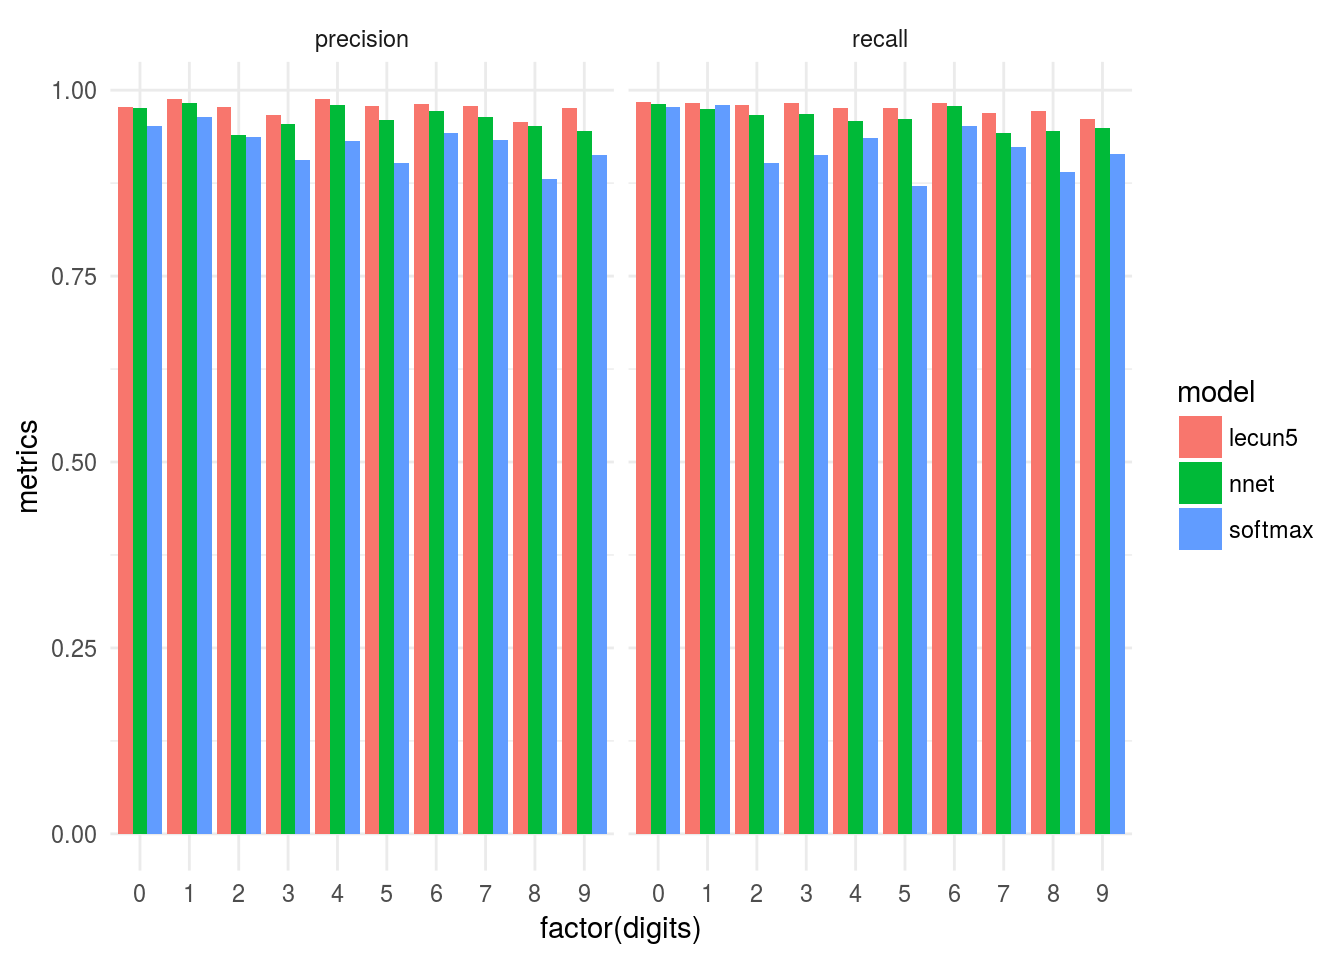
\includegraphics{mml-tutorial_files/figure-latex/calc_metrics-1.pdf}

\chapter{Natural Language Processing}\label{natural-language-processing}

\section{Text Classification}\label{text-classification}

Let's take a look at using \texttt{MML} to estimate a model that would
be very hard to do with \texttt{RevoScaleR}.

In particular, there are virtually no functionality in
\texttt{RevoScaleR} for handling large text data. We will use
\texttt{MML} to transform text data into useful features that we can use
in a logistic regression learner. In order to deal with the high
cardinality of text data, we will use the penalized regression models in
\texttt{MML}.

\subsection{IMDB Data}\label{imdb-data}

Our data is taken from the paper \textbf{Learning Word Vectors for
Sentiment Analysis} written in 2011 by Andrew L. Maas, Raymond E. Daly,
Peter T. Pham, Dan Huang, Andrew Y. Ng, and Christopher Potts. The paper
and data are available here:
\url{http://ai.stanford.edu/~amaas/data/sentiment/}. I've already
downloaded and converted the data into an XDF. Please see the
\texttt{1-ingest-data.R} script if you are interested in the ingestion
process.

\begin{Shaded}
\begin{Highlighting}[]
\KeywordTok{library}\NormalTok{(MicrosoftML)}
\KeywordTok{library}\NormalTok{(tidyverse)}
\KeywordTok{library}\NormalTok{(d3wordcloud)}
\NormalTok{train_xdf <-}\StringTok{ }\KeywordTok{RxXdfData}\NormalTok{(}\StringTok{"data/imdb-train.xdf"}\NormalTok{)}
\NormalTok{test_xdf <-}\StringTok{ }\KeywordTok{RxXdfData}\NormalTok{(}\StringTok{"data/imdb-test.xdf"}\NormalTok{)}
\end{Highlighting}
\end{Shaded}

\subsection{Feature Transformers}\label{feature-transformers}

MicrosoftML has a set of functions for feature engineering. In this
example, let's take a look at creating sparse word vectors.

We'll use the \texttt{featurizeText} function to convert our text data
into numeric columns. In particular, we'll ask for new columns with
tri-grams after removing stopwords, punctuations, and numbers.

We can do this transform directly in our modeling call, and in
particular, we'll train logistic regression models and a fast gradient
boosted tree model:

\begin{Shaded}
\begin{Highlighting}[]
\KeywordTok{system.time}\NormalTok{(logit_model <-}\StringTok{ }\KeywordTok{rxLogisticRegression}\NormalTok{(sentiment }\OperatorTok{~}\StringTok{ }\NormalTok{reviewTran,}
                                                \DataTypeTok{data =}\NormalTok{ train_xdf,}
                                                \DataTypeTok{l1Weight =} \FloatTok{0.05}\NormalTok{,}
                                                \DataTypeTok{l2Weight =} \FloatTok{0.01}\NormalTok{,}
                                                \DataTypeTok{mlTransforms =} 
                                                  \KeywordTok{list}\NormalTok{(}\KeywordTok{featurizeText}\NormalTok{(}
                                                    \DataTypeTok{vars =} \KeywordTok{c}\NormalTok{(}\DataTypeTok{reviewTran =} \StringTok{"review"}\NormalTok{),}
                                                    \DataTypeTok{language =} \StringTok{"English"}\NormalTok{,}
                                                    \DataTypeTok{stopwordsRemover =} \KeywordTok{stopwordsDefault}\NormalTok{(),}
                                                    \DataTypeTok{wordFeatureExtractor =} 
                                                      \KeywordTok{ngramCount}\NormalTok{(}\DataTypeTok{ngramLength =} \DecValTok{3}\NormalTok{,}
                                                                 \DataTypeTok{weighting =} \StringTok{"tfidf"}\NormalTok{,}
                                                                 \DataTypeTok{maxNumTerms =} \FloatTok{1e+09}\NormalTok{),}
                                                    \DataTypeTok{keepNumbers =} \OtherTok{FALSE}\NormalTok{,}
                                                    \DataTypeTok{keepPunctuations =} \OtherTok{FALSE}\NormalTok{)}
\NormalTok{                                                    )}
\NormalTok{                                                )}
\NormalTok{            )}
\end{Highlighting}
\end{Shaded}

\begin{verbatim}
## Not adding a normalizer.
## Automatically converting column 'sentiment' into a factor.
## LBFGS multi-threading will attempt to load dataset into memory. In case of out-of-memory issues, turn off multi-threading by setting trainThreads to 1.
## Beginning optimization
## num vars: 4308438
## improvement criterion: Mean Improvement
## L1 regularization selected 28533 of 4308438 weights.
## Not training a calibrator because it is not needed.
## Elapsed time: 00:02:56.9912387
## Elapsed time: 00:00:52.3671094
\end{verbatim}

\begin{verbatim}
##    user  system elapsed 
##   0.184   0.104 230.296
\end{verbatim}

\begin{Shaded}
\begin{Highlighting}[]
\KeywordTok{system.time}\NormalTok{(fast_trees <-}\StringTok{ }\KeywordTok{rxFastTrees}\NormalTok{(sentiment }\OperatorTok{~}\StringTok{ }\NormalTok{reviewTran,}
                                       \DataTypeTok{data =}\NormalTok{ train_xdf,}
                                       \DataTypeTok{mlTransforms =} 
                                                  \KeywordTok{list}\NormalTok{(}\KeywordTok{featurizeText}\NormalTok{(}
                                                    \DataTypeTok{vars =} \KeywordTok{c}\NormalTok{(}\DataTypeTok{reviewTran =} \StringTok{"review"}\NormalTok{),}
                                                    \DataTypeTok{language =} \StringTok{"English"}\NormalTok{,}
                                                    \DataTypeTok{stopwordsRemover =} \KeywordTok{stopwordsDefault}\NormalTok{(),}
                                                    \DataTypeTok{wordFeatureExtractor =} 
                                                      \KeywordTok{ngramCount}\NormalTok{(}\DataTypeTok{ngramLength =} \DecValTok{3}\NormalTok{,}
                                                                 \DataTypeTok{weighting =} \StringTok{"tfidf"}\NormalTok{,}
                                                                 \DataTypeTok{maxNumTerms =} \FloatTok{1e+09}\NormalTok{),}
                                                    \DataTypeTok{keepNumbers =} \OtherTok{FALSE}\NormalTok{,}
                                                    \DataTypeTok{keepPunctuations =} \OtherTok{FALSE}\NormalTok{)}
\NormalTok{                                                    )}
\NormalTok{                                      )}
\NormalTok{            )}
\end{Highlighting}
\end{Shaded}

\begin{verbatim}
## Not adding a normalizer.
## Automatically converting column 'sentiment' into a factor.
## Making per-feature arrays
## Changing data from row-wise to column-wise
## Processed 25000 instances
## Binning and forming Feature objects
## Reserved memory for tree learner: 304827068 bytes
## Starting to train ...
## Not training a calibrator because it is not needed.
## Elapsed time: 00:01:09.6558035
\end{verbatim}

\begin{verbatim}
##    user  system elapsed 
##   0.020   0.068  69.839
\end{verbatim}

Now that we have our trained model, we can do some visualizations. For
example, for the elastic net, we can visualize the coefficients.

\begin{Shaded}
\begin{Highlighting}[]
\NormalTok{logit_cof <-}\StringTok{ }\KeywordTok{coefficients}\NormalTok{(logit_model)}
\NormalTok{coefs <-}\StringTok{ }\KeywordTok{data.frame}\NormalTok{(}\DataTypeTok{coef =}\NormalTok{ logit_cof, }\DataTypeTok{word =} \KeywordTok{names}\NormalTok{(logit_cof))}
\NormalTok{coefs <-}\StringTok{ }\KeywordTok{tbl_df}\NormalTok{(coefs)}

\NormalTok{coefs <-}\StringTok{ }\NormalTok{coefs }\OperatorTok
\StringTok{  }\KeywordTok{filter}\NormalTok{(word }\OperatorTok{!=}\StringTok{ "(Bias)"}\NormalTok{) }\OperatorTok\StringTok{ }
\StringTok{  }\KeywordTok{mutate}\NormalTok{(}\DataTypeTok{abs_value =} \KeywordTok{abs}\NormalTok{(coef), }
         \DataTypeTok{sentiment =} \KeywordTok{ifelse}\NormalTok{(coef }\OperatorTok{>}\StringTok{ }\DecValTok{0}\NormalTok{, }\StringTok{"Positive"}\NormalTok{, }\StringTok{"Negative"}\NormalTok{), }
         \DataTypeTok{score =} \KeywordTok{round}\NormalTok{(abs_value, }\DecValTok{0}\NormalTok{)) }\OperatorTok\StringTok{ }
\StringTok{  }\KeywordTok{arrange}\NormalTok{(}\KeywordTok{desc}\NormalTok{(abs_value)) }\OperatorTok\StringTok{ }\KeywordTok{slice}\NormalTok{(}\DecValTok{1}\OperatorTok{:}\DecValTok{100}\NormalTok{) }


\KeywordTok{library}\NormalTok{(ggplot2)}
\KeywordTok{library}\NormalTok{(ggrepel)}

\NormalTok{coefs }\OperatorTok\StringTok{ }
\StringTok{  }\NormalTok{ggplot }\OperatorTok{+}
\StringTok{    }\KeywordTok{aes}\NormalTok{(}\DataTypeTok{x =} \DecValTok{1}\NormalTok{, }\DataTypeTok{y =} \DecValTok{1}\NormalTok{, }\DataTypeTok{colour =}\NormalTok{ sentiment, }\DataTypeTok{size =}\NormalTok{ score, }\DataTypeTok{label =}\NormalTok{ word) }\OperatorTok{+}
\StringTok{    }\KeywordTok{geom_text_repel}\NormalTok{(}\DataTypeTok{segment.size =} \DecValTok{0}\NormalTok{, }\DataTypeTok{force =} \DecValTok{10}\NormalTok{) }\OperatorTok{+}
\StringTok{    }\KeywordTok{scale_size}\NormalTok{(}\DataTypeTok{range =} \KeywordTok{c}\NormalTok{(}\DecValTok{2}\NormalTok{, }\DecValTok{15}\NormalTok{), }\DataTypeTok{guide =} \OtherTok{FALSE}\NormalTok{) }\OperatorTok{+}
\StringTok{    }\KeywordTok{scale_y_continuous}\NormalTok{(}\DataTypeTok{breaks =} \OtherTok{NULL}\NormalTok{) }\OperatorTok{+}
\StringTok{    }\KeywordTok{scale_x_continuous}\NormalTok{(}\DataTypeTok{breaks =} \OtherTok{NULL}\NormalTok{) }\OperatorTok{+}
\StringTok{    }\KeywordTok{labs}\NormalTok{(}\DataTypeTok{x =} \StringTok{''}\NormalTok{, }\DataTypeTok{y =} \StringTok{''}\NormalTok{) }\OperatorTok{+}
\StringTok{    }\KeywordTok{theme_classic}\NormalTok{() }\OperatorTok{+}
\StringTok{    }\KeywordTok{facet_wrap}\NormalTok{(}\OperatorTok{~}\NormalTok{sentiment)}
\end{Highlighting}
\end{Shaded}

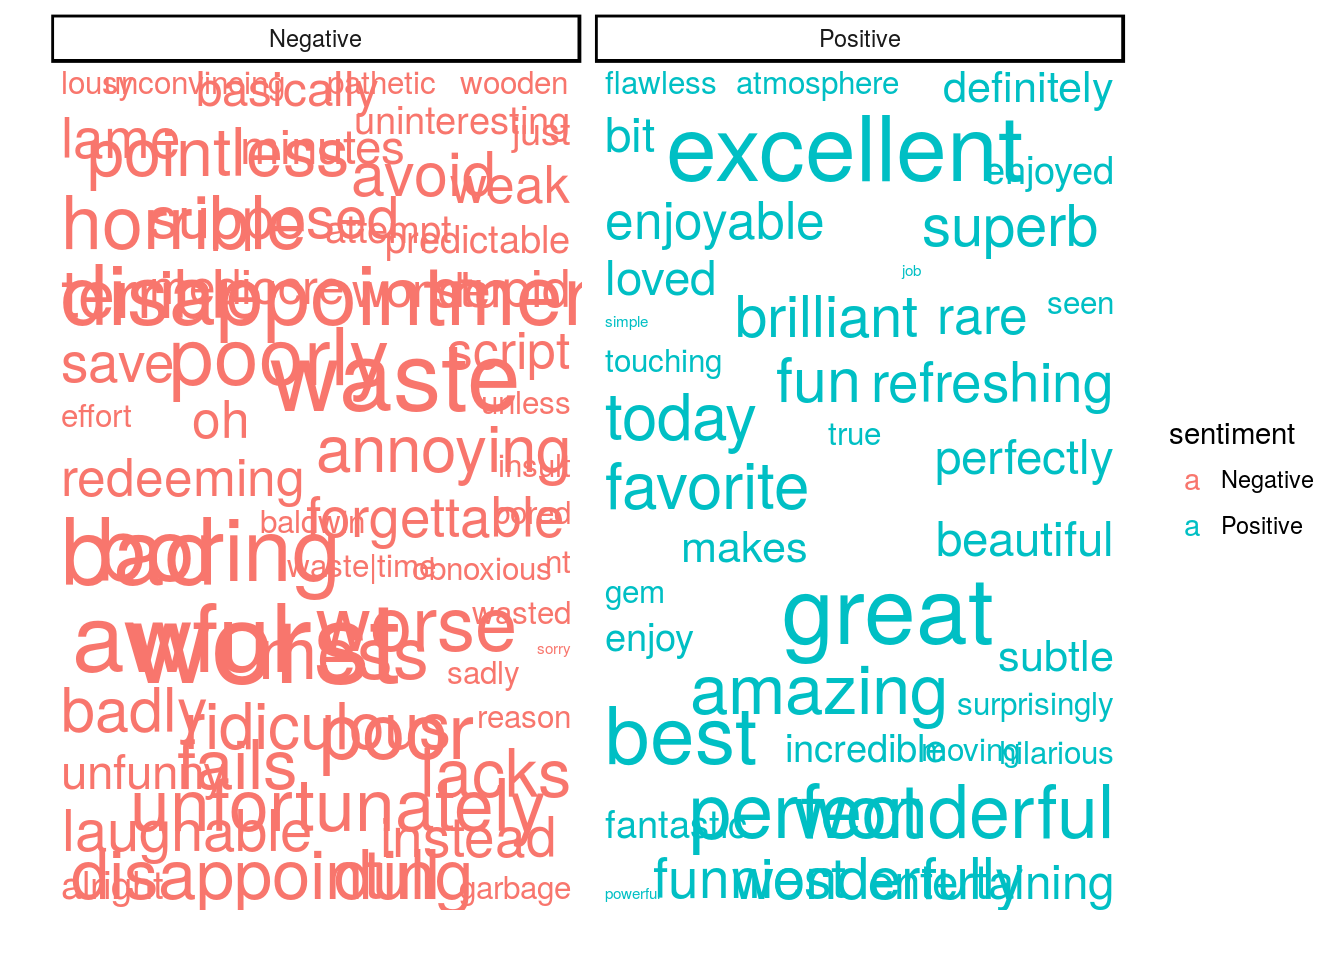
\includegraphics{mml-tutorial_files/figure-latex/coefs-1.pdf}

Let's try and makea more interactive visual. We'll use \texttt{purrr}
again to map our coefficients to the beautiful
\href{https://github.com/jbkunst/d3wordcloud}{d3wordcloud} package

\begin{Shaded}
\begin{Highlighting}[]
\NormalTok{coefs }\OperatorTok\StringTok{ }
\StringTok{  }\KeywordTok{split}\NormalTok{(.}\OperatorTok{$}\NormalTok{sentiment) }\OperatorTok\StringTok{ }
\StringTok{  }\NormalTok{purrr}\OperatorTok{::}\KeywordTok{map}\NormalTok{( }\OperatorTok{~}\StringTok{ }\KeywordTok{d3wordcloud}\NormalTok{(.}\OperatorTok{$}\NormalTok{word, .}\OperatorTok{$}\NormalTok{score, }\DataTypeTok{tooltip =} \OtherTok{TRUE}\NormalTok{)) ->}\StringTok{ }\NormalTok{d3_graphs}

\NormalTok{d3_graphs[[}\DecValTok{1}\NormalTok{]]}
\end{Highlighting}
\end{Shaded}

\hypertarget{htmlwidget-336dfbd44998e6742520}{}

\begin{Shaded}
\begin{Highlighting}[]
\NormalTok{d3_graphs[[}\DecValTok{2}\NormalTok{]]}
\end{Highlighting}
\end{Shaded}

\hypertarget{htmlwidget-06bc5f93d3d0df1cf391}{}

\subsection{Testing the Logit Model}\label{testing-the-logit-model}

In order to predict our classifer on test data, we will use the
\texttt{mxPredict} function from the \texttt{MML} package.

\begin{Shaded}
\begin{Highlighting}[]
\NormalTok{predictions <-}\StringTok{ }\KeywordTok{rxPredict}\NormalTok{(logit_model, }\DataTypeTok{data =}\NormalTok{ test_xdf, }\DataTypeTok{extraVarsToWrite =} \StringTok{"sentiment"}\NormalTok{)}
\end{Highlighting}
\end{Shaded}

\begin{verbatim}
## Elapsed time: 00:00:26.5864958
\end{verbatim}

\begin{Shaded}
\begin{Highlighting}[]
\NormalTok{roc_results <-}\StringTok{ }\KeywordTok{rxRoc}\NormalTok{(}\DataTypeTok{actualVarName =} \StringTok{"sentiment"}\NormalTok{, }\DataTypeTok{predVarNames =} \StringTok{"Probability.1"}\NormalTok{, }\DataTypeTok{data =}\NormalTok{ predictions)}
\NormalTok{roc_results}\OperatorTok{$}\NormalTok{predVarName <-}\StringTok{ }\KeywordTok{factor}\NormalTok{(roc_results}\OperatorTok{$}\NormalTok{predVarName)}
\KeywordTok{plot}\NormalTok{(roc_results)}
\end{Highlighting}
\end{Shaded}

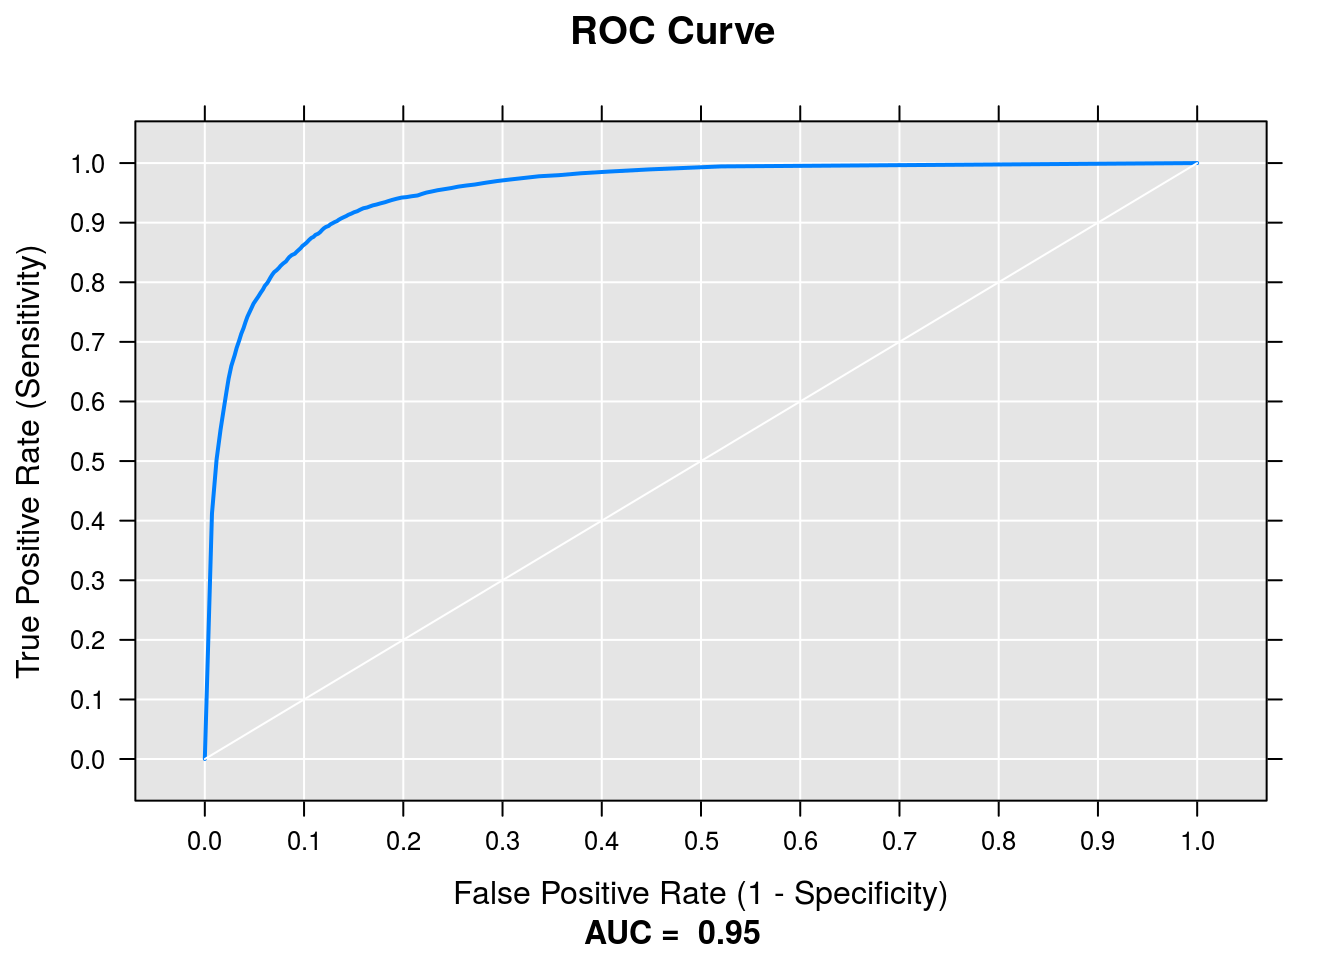
\includegraphics{mml-tutorial_files/figure-latex/scorelogit-1.pdf}

\subsection{Testing the Fast Trees
Model}\label{testing-the-fast-trees-model}

\begin{Shaded}
\begin{Highlighting}[]
\NormalTok{predictions <-}\StringTok{ }\KeywordTok{rxPredict}\NormalTok{(fast_trees, }\DataTypeTok{data =}\NormalTok{ test_xdf, }\DataTypeTok{extraVarsToWrite =} \StringTok{"sentiment"}\NormalTok{)}
\end{Highlighting}
\end{Shaded}

\begin{verbatim}
## Elapsed time: 00:00:29.4280653
\end{verbatim}

\begin{Shaded}
\begin{Highlighting}[]
\NormalTok{roc_results <-}\StringTok{ }\KeywordTok{rxRoc}\NormalTok{(}\DataTypeTok{actualVarName =} \StringTok{"sentiment"}\NormalTok{, }\DataTypeTok{predVarNames =} \StringTok{"Probability.1"}\NormalTok{, }\DataTypeTok{data =}\NormalTok{ predictions)}
\NormalTok{roc_results}\OperatorTok{$}\NormalTok{predVarName <-}\StringTok{ }\KeywordTok{factor}\NormalTok{(roc_results}\OperatorTok{$}\NormalTok{predVarName)}
\KeywordTok{plot}\NormalTok{(roc_results)}
\end{Highlighting}
\end{Shaded}

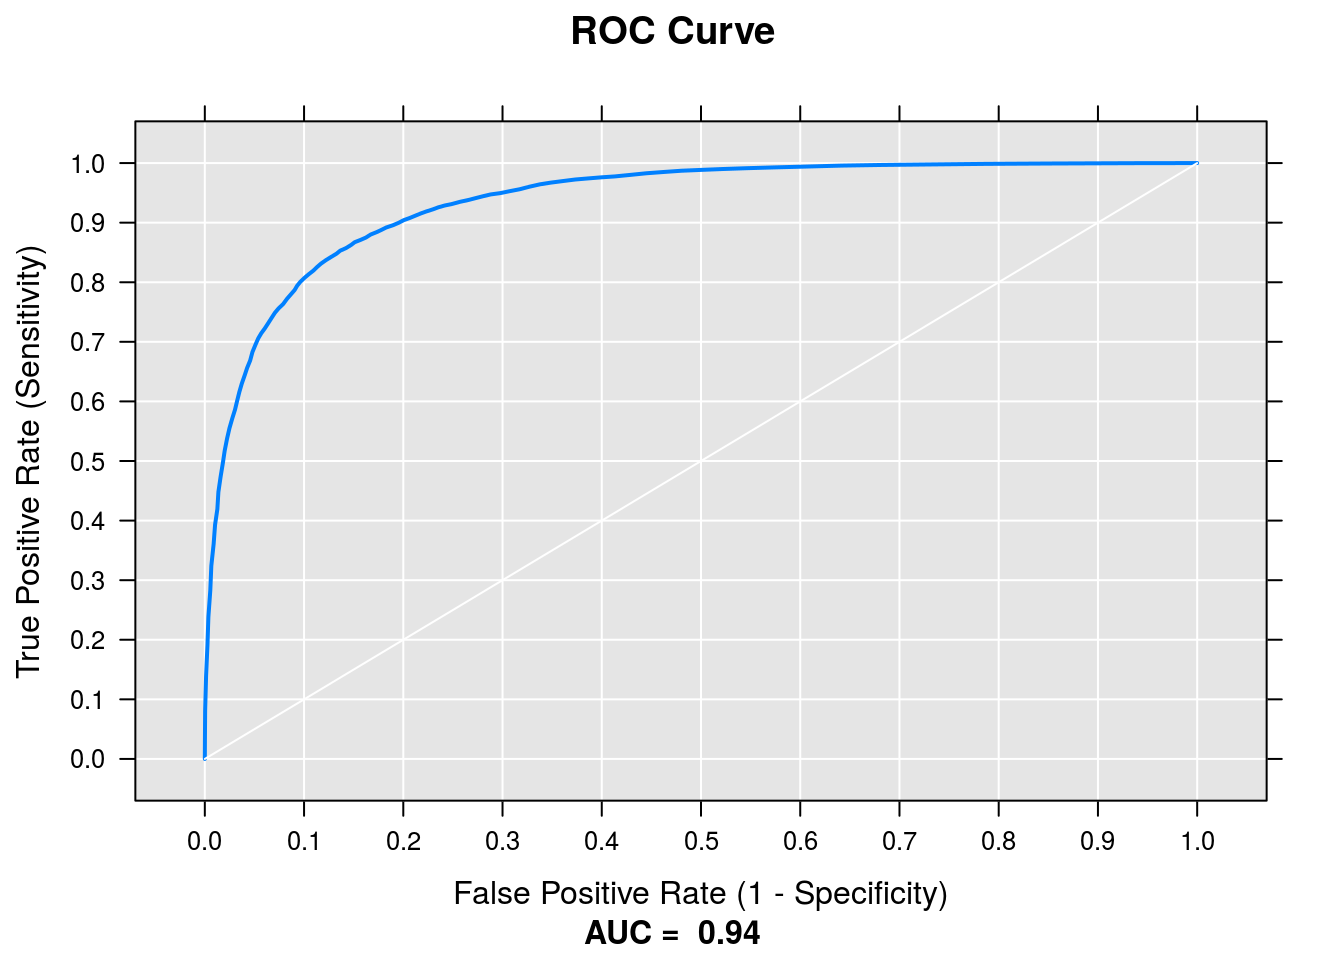
\includegraphics{mml-tutorial_files/figure-latex/score_sdca-1.pdf}

\section{Neural Networks}\label{neural-networks}

Let's try to estimate another binary classifier from this dataset, but
with a Neural Network architecture rather than a logistic regression
model.

In the following chunk, we call our neural network model, and set the
optimizer to be a stochastic gradient descent optimizer with a learning
rate of 0.2. Furthermore, we use the \texttt{type} argument to ensure we
are learning a binary classifier. By default our network architecture
will have 100 hidden nodes.

\begin{Shaded}
\begin{Highlighting}[]
\NormalTok{nn_sentiment <-}\StringTok{ }\KeywordTok{rxNeuralNet}\NormalTok{(sentiment }\OperatorTok{~}\StringTok{ }\NormalTok{reviewTran,}
                            \DataTypeTok{data =}\NormalTok{ train_xdf,}
                            \DataTypeTok{type =} \StringTok{"binary"}\NormalTok{,}
                            \DataTypeTok{mlTransforms =} \KeywordTok{list}\NormalTok{(}\KeywordTok{featurizeText}\NormalTok{(}\DataTypeTok{vars =} \KeywordTok{c}\NormalTok{(}\DataTypeTok{reviewTran =} \StringTok{"review"}\NormalTok{),}
                                                         \DataTypeTok{language =} \StringTok{"English"}\NormalTok{,}
                                                         \DataTypeTok{stopwordsRemover =} \KeywordTok{stopwordsDefault}\NormalTok{(),}
                                                         \DataTypeTok{keepPunctuations =} \OtherTok{FALSE}\NormalTok{)),}
                          \CommentTok{# acceleration = "gpu",}
                          \DataTypeTok{miniBatchSize =} \DecValTok{4}\NormalTok{)}
\end{Highlighting}
\end{Shaded}

\begin{verbatim}
## Not adding a normalizer.
## Automatically converting column 'sentiment' into a factor.
## Using: SSE Math
## Warning: Math acceleration mode not compatible with mini-batches. Setting batch size to 1.
## ***** Net definition *****
##   input Data [74398];
##   hidden H [100] sigmoid { // Depth 1
##     from Data all;
##   }
##   output Result [1] sigmoid { // Depth 0
##     from H all;
##   }
## ***** End net definition *****
## Input count: 74398
## Output count: 1
## Output Function: Sigmoid
## Loss Function: CrossEntropy
## PreTrainer: NoPreTrainer
## ___________________________________________________________________
## Starting training...
## Learning rate: 0.001000
## Momentum: 0.000000
## InitWtsDiameter: 0.100000
## ___________________________________________________________________
## Initializing 1 Hidden Layers, 7440001 Weights...
## Estimated Pre-training MeanError = 0.704585
## Iter:1/100, MeanErr=0.694443(-1.44%), 125415.57M WeightUpdates/sec
## Iter:2/100, MeanErr=0.694329(-0.02%), 130494.76M WeightUpdates/sec
## Iter:3/100, MeanErr=0.694192(-0.02%), 132241.61M WeightUpdates/sec
## Iter:4/100, MeanErr=0.694030(-0.02%), 131118.71M WeightUpdates/sec
## Iter:5/100, MeanErr=0.694215(0.03%), 128647.66M WeightUpdates/sec
## Iter:6/100, MeanErr=0.693894(-0.05%), 126401.64M WeightUpdates/sec
## Iter:7/100, MeanErr=0.693471(-0.06%), 128879.81M WeightUpdates/sec
## Iter:8/100, MeanErr=0.692859(-0.09%), 134158.70M WeightUpdates/sec
## Iter:9/100, MeanErr=0.692376(-0.07%), 127289.61M WeightUpdates/sec
## Iter:10/100, MeanErr=0.691277(-0.16%), 125183.79M WeightUpdates/sec
## Iter:11/100, MeanErr=0.690757(-0.08%), 124604.89M WeightUpdates/sec
## Iter:12/100, MeanErr=0.689446(-0.19%), 127705.30M WeightUpdates/sec
## Iter:13/100, MeanErr=0.687619(-0.26%), 128392.39M WeightUpdates/sec
## Iter:14/100, MeanErr=0.685640(-0.29%), 130021.94M WeightUpdates/sec
## Iter:15/100, MeanErr=0.683191(-0.36%), 131894.86M WeightUpdates/sec
## Iter:16/100, MeanErr=0.680226(-0.43%), 136040.52M WeightUpdates/sec
## Iter:17/100, MeanErr=0.676299(-0.58%), 134689.88M WeightUpdates/sec
## Iter:18/100, MeanErr=0.671884(-0.65%), 126922.87M WeightUpdates/sec
## Iter:19/100, MeanErr=0.666806(-0.76%), 126259.57M WeightUpdates/sec
## Iter:20/100, MeanErr=0.660784(-0.90%), 128367.22M WeightUpdates/sec
## Iter:21/100, MeanErr=0.653908(-1.04%), 127823.27M WeightUpdates/sec
## Iter:22/100, MeanErr=0.645968(-1.21%), 125449.66M WeightUpdates/sec
## Iter:23/100, MeanErr=0.637465(-1.32%), 128992.18M WeightUpdates/sec
## Iter:24/100, MeanErr=0.628361(-1.43%), 128921.78M WeightUpdates/sec
## Iter:25/100, MeanErr=0.618374(-1.59%), 128686.66M WeightUpdates/sec
## Iter:26/100, MeanErr=0.607630(-1.74%), 125625.10M WeightUpdates/sec
## Iter:27/100, MeanErr=0.596812(-1.78%), 126844.28M WeightUpdates/sec
## Iter:28/100, MeanErr=0.585189(-1.95%), 127762.36M WeightUpdates/sec
## Iter:29/100, MeanErr=0.573419(-2.01%), 136768.58M WeightUpdates/sec
## Iter:30/100, MeanErr=0.561505(-2.08%), 136910.76M WeightUpdates/sec
## Iter:31/100, MeanErr=0.549777(-2.09%), 135253.79M WeightUpdates/sec
## Iter:32/100, MeanErr=0.538191(-2.11%), 138856.24M WeightUpdates/sec
## Iter:33/100, MeanErr=0.526569(-2.16%), 133778.06M WeightUpdates/sec
## Iter:34/100, MeanErr=0.515547(-2.09%), 126691.70M WeightUpdates/sec
## Iter:35/100, MeanErr=0.504761(-2.09%), 130933.52M WeightUpdates/sec
## Iter:36/100, MeanErr=0.494128(-2.11%), 126065.20M WeightUpdates/sec
## Iter:37/100, MeanErr=0.484511(-1.95%), 127670.71M WeightUpdates/sec
## Iter:38/100, MeanErr=0.474862(-1.99%), 126004.34M WeightUpdates/sec
## Iter:39/100, MeanErr=0.465674(-1.93%), 128223.43M WeightUpdates/sec
## Iter:40/100, MeanErr=0.456896(-1.88%), 129744.36M WeightUpdates/sec
## Iter:41/100, MeanErr=0.448901(-1.75%), 131564.48M WeightUpdates/sec
## Iter:42/100, MeanErr=0.441171(-1.72%), 128833.48M WeightUpdates/sec
## Iter:43/100, MeanErr=0.433480(-1.74%), 130683.41M WeightUpdates/sec
## Iter:44/100, MeanErr=0.426293(-1.66%), 132297.95M WeightUpdates/sec
## Iter:45/100, MeanErr=0.419575(-1.58%), 126329.45M WeightUpdates/sec
## Iter:46/100, MeanErr=0.413401(-1.47%), 127071.73M WeightUpdates/sec
## Iter:47/100, MeanErr=0.406957(-1.56%), 124416.71M WeightUpdates/sec
## Iter:48/100, MeanErr=0.401313(-1.39%), 125157.72M WeightUpdates/sec
## Iter:49/100, MeanErr=0.395543(-1.44%), 125105.73M WeightUpdates/sec
## Iter:50/100, MeanErr=0.390251(-1.34%), 126154.53M WeightUpdates/sec
## Iter:51/100, MeanErr=0.385156(-1.31%), 122496.72M WeightUpdates/sec
## Iter:52/100, MeanErr=0.380155(-1.30%), 134559.53M WeightUpdates/sec
## Iter:53/100, MeanErr=0.375252(-1.29%), 124359.93M WeightUpdates/sec
## Iter:54/100, MeanErr=0.371025(-1.13%), 127304.69M WeightUpdates/sec
## Iter:55/100, MeanErr=0.366597(-1.19%), 125388.90M WeightUpdates/sec
## Iter:56/100, MeanErr=0.362269(-1.18%), 126106.61M WeightUpdates/sec
## Iter:57/100, MeanErr=0.358292(-1.10%), 133691.33M WeightUpdates/sec
## Iter:58/100, MeanErr=0.354345(-1.10%), 132204.62M WeightUpdates/sec
## Iter:59/100, MeanErr=0.350553(-1.07%), 125161.28M WeightUpdates/sec
## Iter:60/100, MeanErr=0.346730(-1.09%), 137173.58M WeightUpdates/sec
## Iter:61/100, MeanErr=0.343272(-1.00%), 126914.94M WeightUpdates/sec
## Iter:62/100, MeanErr=0.339770(-1.02%), 135821.28M WeightUpdates/sec
## Iter:63/100, MeanErr=0.336230(-1.04%), 134923.71M WeightUpdates/sec
## Iter:64/100, MeanErr=0.333191(-0.90%), 126294.75M WeightUpdates/sec
## Iter:65/100, MeanErr=0.330051(-0.94%), 126416.33M WeightUpdates/sec
## Iter:66/100, MeanErr=0.326981(-0.93%), 124905.46M WeightUpdates/sec
## Iter:67/100, MeanErr=0.323995(-0.91%), 124701.09M WeightUpdates/sec
## Iter:68/100, MeanErr=0.321182(-0.87%), 125438.43M WeightUpdates/sec
## Iter:69/100, MeanErr=0.318367(-0.88%), 127085.70M WeightUpdates/sec
## Iter:70/100, MeanErr=0.315463(-0.91%), 122849.20M WeightUpdates/sec
## Iter:71/100, MeanErr=0.313039(-0.77%), 125325.57M WeightUpdates/sec
## Iter:72/100, MeanErr=0.310367(-0.85%), 126297.57M WeightUpdates/sec
## Iter:73/100, MeanErr=0.307799(-0.83%), 125278.45M WeightUpdates/sec
## Iter:74/100, MeanErr=0.305068(-0.89%), 127582.72M WeightUpdates/sec
## Iter:75/100, MeanErr=0.302958(-0.69%), 128067.18M WeightUpdates/sec
## Iter:76/100, MeanErr=0.300405(-0.84%), 127380.58M WeightUpdates/sec
## Iter:77/100, MeanErr=0.297983(-0.81%), 125099.27M WeightUpdates/sec
## Iter:78/100, MeanErr=0.295944(-0.68%), 127625.57M WeightUpdates/sec
## Iter:79/100, MeanErr=0.293907(-0.69%), 125770.09M WeightUpdates/sec
## Iter:80/100, MeanErr=0.291620(-0.78%), 132136.38M WeightUpdates/sec
## Iter:81/100, MeanErr=0.289745(-0.64%), 125433.57M WeightUpdates/sec
## Iter:82/100, MeanErr=0.287662(-0.72%), 127810.74M WeightUpdates/sec
## Iter:83/100, MeanErr=0.285591(-0.72%), 128472.66M WeightUpdates/sec
## Iter:84/100, MeanErr=0.283583(-0.70%), 126612.25M WeightUpdates/sec
## Iter:85/100, MeanErr=0.281815(-0.62%), 127929.90M WeightUpdates/sec
## Iter:86/100, MeanErr=0.279837(-0.70%), 126589.35M WeightUpdates/sec
## Iter:87/100, MeanErr=0.278120(-0.61%), 130552.71M WeightUpdates/sec
## Iter:88/100, MeanErr=0.276277(-0.66%), 127951.54M WeightUpdates/sec
## Iter:89/100, MeanErr=0.274533(-0.63%), 130041.89M WeightUpdates/sec
## Iter:90/100, MeanErr=0.272938(-0.58%), 127955.84M WeightUpdates/sec
## Iter:91/100, MeanErr=0.270917(-0.74%), 126596.53M WeightUpdates/sec
## Iter:92/100, MeanErr=0.269519(-0.52%), 127407.53M WeightUpdates/sec
## Iter:93/100, MeanErr=0.267711(-0.67%), 128363.02M WeightUpdates/sec
## Iter:94/100, MeanErr=0.266137(-0.59%), 125147.07M WeightUpdates/sec
## Iter:95/100, MeanErr=0.264770(-0.51%), 126902.31M WeightUpdates/sec
## Iter:96/100, MeanErr=0.262845(-0.73%), 128173.66M WeightUpdates/sec
## Iter:97/100, MeanErr=0.261513(-0.51%), 127248.96M WeightUpdates/sec
## Iter:98/100, MeanErr=0.259934(-0.60%), 126299.90M WeightUpdates/sec
## Iter:99/100, MeanErr=0.258394(-0.59%), 126134.74M WeightUpdates/sec
## Iter:100/100, MeanErr=0.257150(-0.48%), 134732.80M WeightUpdates/sec
## Done!
## Estimated Post-training MeanError = 0.256146
## ___________________________________________________________________
## Not training a calibrator because it is not needed.
## Elapsed time: 00:02:34.9539664
\end{verbatim}

\subsection{Scoring the Neural Net}\label{scoring-the-neural-net}

We can similary score our results from the neural network model

\begin{Shaded}
\begin{Highlighting}[]
\NormalTok{predictions <-}\StringTok{ }\KeywordTok{rxPredict}\NormalTok{(nn_sentiment, }\DataTypeTok{data =}\NormalTok{ test_xdf, }\DataTypeTok{extraVarsToWrite =} \StringTok{"sentiment"}\NormalTok{)}
\end{Highlighting}
\end{Shaded}

\begin{verbatim}
## Elapsed time: 00:00:12.8994661
\end{verbatim}

\begin{Shaded}
\begin{Highlighting}[]
\NormalTok{roc_results <-}\StringTok{ }\KeywordTok{rxRoc}\NormalTok{(}\DataTypeTok{actualVarName =} \StringTok{"sentiment"}\NormalTok{, }\DataTypeTok{predVarNames =} \StringTok{"Probability.1"}\NormalTok{, }\DataTypeTok{data =}\NormalTok{ predictions)}
\NormalTok{roc_results}\OperatorTok{$}\NormalTok{predVarName <-}\StringTok{ }\KeywordTok{factor}\NormalTok{(roc_results}\OperatorTok{$}\NormalTok{predVarName)}
\KeywordTok{plot}\NormalTok{(roc_results)}
\end{Highlighting}
\end{Shaded}

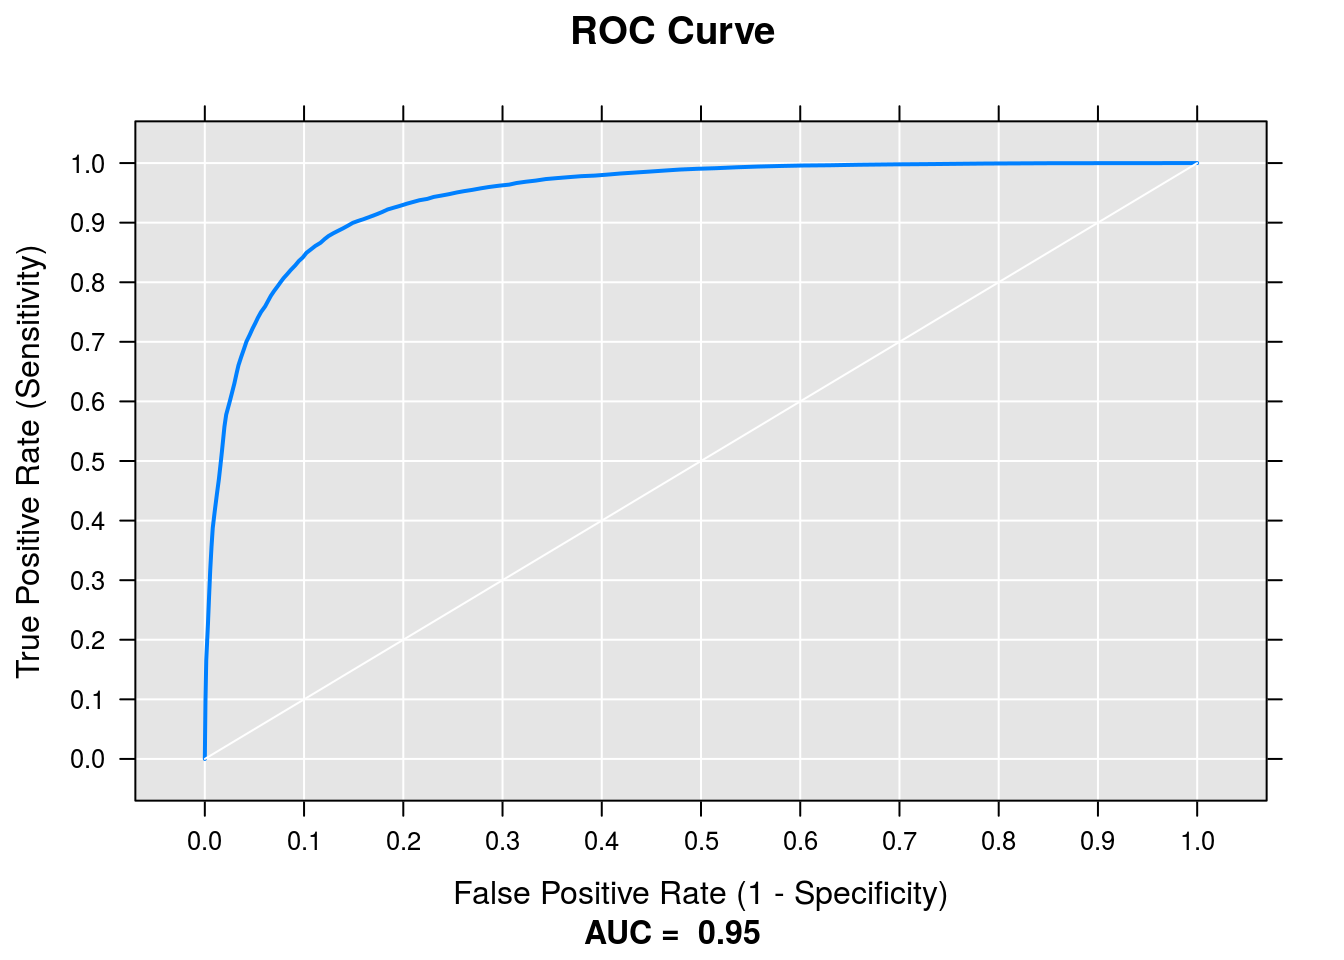
\includegraphics{mml-tutorial_files/figure-latex/predsentiment-1.pdf}

\section{Exercises}\label{exercises-2}

\begin{enumerate}
\def\labelenumi{\arabic{enumi}.}
\tightlist
\item
  The Rscript
  \href{../Rscripts/9-Other-Sentiment-Datasets.R}{Rscripts/9-Other-Sentiment-Datasets.R}
  has two additional datasets with reviews and ratings (binarized). Try
  the above analysis on the other two datasets.
\end{enumerate}

\chapter{Transfer Learning with Pre-Trained Deep Neural Network
Architectures -- The Shallow End of Deep
Learning}\label{transfer-learning-with-pre-trained-deep-neural-network-architectures-the-shallow-end-of-deep-learning}

\section{Pre-Trained Models}\label{pre-trained-models}

Transfer learning is a pretty incredible method for learning expressive
models without having to train a deep architecture from scratch. In some
ways, it's nearly a ``free-lunch'': take a pre-built model trained for
weeks on a large image corpus, and reuse the features from that model
for your domain-specific task.

\texttt{MicrosoftML} ships with a number of pre-trained DNNs on the
\href{http://www.image-net.org/}{ImageNet} challenge dataset.

\begin{Shaded}
\begin{Highlighting}[]
\NormalTok{AlexNetFeatures <-}\StringTok{ }\KeywordTok{read.csv}\NormalTok{(}\KeywordTok{system.file}\NormalTok{(}
  \StringTok{"extdata/ImageAnalyticsTestData/featurizeImage_alexnet_output.csv"}\NormalTok{,}
  \DataTypeTok{package =} \StringTok{"MicrosoftML"}\NormalTok{), }
  \DataTypeTok{header =} \OtherTok{FALSE}\NormalTok{)}

\NormalTok{ResNet18Features <-}\StringTok{ }\KeywordTok{read.csv}\NormalTok{(}\KeywordTok{system.file}\NormalTok{(}
  \StringTok{"extdata/ImageAnalyticsTestData/featurizeImage_resnet18_output.csv"}\NormalTok{,}
  \DataTypeTok{package =} \StringTok{"MicrosoftML"}\NormalTok{),}
  \DataTypeTok{header =} \OtherTok{FALSE}\NormalTok{)}

\NormalTok{ResNet50Features <-}\StringTok{ }\KeywordTok{read.csv}\NormalTok{(}\KeywordTok{system.file}\NormalTok{(}
  \StringTok{"extdata/ImageAnalyticsTestData/featurizeImage_resnet50_output.csv"}\NormalTok{,}
  \DataTypeTok{package =} \StringTok{"MicrosoftML"}\NormalTok{), }
  \DataTypeTok{header =} \OtherTok{FALSE}\NormalTok{)}

\NormalTok{ResNet101Features <-}\StringTok{ }\KeywordTok{read.csv}\NormalTok{(}\KeywordTok{system.file}\NormalTok{(}
  \StringTok{"extdata/ImageAnalyticsTestData/featurizeImage_resnet101_output.csv"}\NormalTok{,}
  \DataTypeTok{package =} \StringTok{"MicrosoftML"}\NormalTok{), }
  \DataTypeTok{header =} \OtherTok{FALSE}\NormalTok{)}

\KeywordTok{lapply}\NormalTok{(}\KeywordTok{list}\NormalTok{(AlexNetFeatures, ResNet18Features, ResNet50Features, ResNet101Features),}
\NormalTok{       dim)}
\end{Highlighting}
\end{Shaded}

\begin{verbatim}
## [[1]]
## [1]    2 4097
## 
## [[2]]
## [1]   2 513
## 
## [[3]]
## [1]    2 2049
## 
## [[4]]
## [1]    2 2049
\end{verbatim}

\section{CMU Faces Dataset}\label{cmu-faces-dataset}

For this notebook, we'll use the
\href{http://archive.ics.uci.edu/ml/datasets/CMU+Face+Images}{CMU Faces
dataset} compiled by Tom Mitchell and his students way back in 1999.

\begin{Shaded}
\begin{Highlighting}[]
\CommentTok{# get paths to full-resolution images, regex"[[:alpha:]_]+.pgm"}
\CommentTok{# see: http://archive.ics.uci.edu/ml/machine-learning-databases/faces-mld/faces.data.html for image resolution info}
\CommentTok{# prepare training and testing data, extract labels: left VS right}
\NormalTok{l <-}\StringTok{ "left"}
\NormalTok{r <-}\StringTok{ "right"}
\NormalTok{imgs_l <-}\StringTok{ }\KeywordTok{list.files}\NormalTok{(}\StringTok{"data/faces"}\NormalTok{,}
                     \DataTypeTok{pattern =} \KeywordTok{paste0}\NormalTok{(l, }\StringTok{"[[:alpha:]_]+.pgm"}\NormalTok{),}
                     \DataTypeTok{recursive =} \OtherTok{TRUE}\NormalTok{, }\DataTypeTok{full.names =} \OtherTok{TRUE}\NormalTok{)}
\NormalTok{imgs_r <-}\StringTok{ }\KeywordTok{list.files}\NormalTok{(}\StringTok{"data/faces"}\NormalTok{,}
                     \DataTypeTok{pattern =} \KeywordTok{paste0}\NormalTok{(r, }\StringTok{"[[:alpha:]_]+.pgm"}\NormalTok{), }
                     \DataTypeTok{recursive =} \OtherTok{TRUE}\NormalTok{, }\DataTypeTok{full.names =} \OtherTok{TRUE}\NormalTok{)}

\NormalTok{l_l <-}\StringTok{ }\KeywordTok{length}\NormalTok{(imgs_l)}
\NormalTok{l_r <-}\StringTok{ }\KeywordTok{length}\NormalTok{(imgs_r)}

\NormalTok{train_l_l <-}\StringTok{ }\KeywordTok{ceiling}\NormalTok{(l_l }\OperatorTok{/}\StringTok{ }\DecValTok{2}\NormalTok{) }\CommentTok{#get balanced train and test set, split each class by half}
\NormalTok{train_l_r <-}\StringTok{ }\KeywordTok{ceiling}\NormalTok{(l_r }\OperatorTok{/}\StringTok{ }\DecValTok{2}\NormalTok{)}

\NormalTok{trainIndex_l <-}\StringTok{ }\KeywordTok{sample}\NormalTok{(l_l, train_l_l)}
\NormalTok{trainIndex_r <-}\StringTok{ }\KeywordTok{sample}\NormalTok{(l_r, train_l_r)}

\NormalTok{train_df <-}\StringTok{ }\KeywordTok{data.frame}\NormalTok{(}\DataTypeTok{Path =} \KeywordTok{c}\NormalTok{(imgs_l[trainIndex_l], imgs_r[trainIndex_r]),}
                       \DataTypeTok{Label =} \KeywordTok{c}\NormalTok{(}\KeywordTok{rep}\NormalTok{(}\OtherTok{TRUE}\NormalTok{, train_l_l), }\KeywordTok{rep}\NormalTok{(}\OtherTok{FALSE}\NormalTok{, train_l_r)),}
                       \DataTypeTok{stringsAsFactors =} \OtherTok{FALSE}\NormalTok{)}

\NormalTok{test_df <-}\StringTok{ }\KeywordTok{data.frame}\NormalTok{(}\DataTypeTok{Path =} \KeywordTok{c}\NormalTok{(imgs_l[}\OperatorTok{-}\NormalTok{trainIndex_l], imgs_r[}\OperatorTok{-}\NormalTok{trainIndex_r]),}
                      \DataTypeTok{Label =} \KeywordTok{c}\NormalTok{(}\KeywordTok{rep}\NormalTok{(}\OtherTok{TRUE}\NormalTok{, l_l}\OperatorTok{-}\NormalTok{train_l_l), }\KeywordTok{rep}\NormalTok{(}\OtherTok{FALSE}\NormalTok{, l_r}\OperatorTok{-}\NormalTok{train_l_r)),}
                      \DataTypeTok{stringsAsFactors =} \OtherTok{FALSE}\NormalTok{)}

\NormalTok{train_df <-}\StringTok{ }\NormalTok{train_df[}\KeywordTok{sample}\NormalTok{(}\KeywordTok{nrow}\NormalTok{(train_df)),]}
\NormalTok{test_df <-}\StringTok{ }\NormalTok{test_df[}\KeywordTok{sample}\NormalTok{(}\KeywordTok{nrow}\NormalTok{(test_df)),]}

\KeywordTok{lapply}\NormalTok{(}\KeywordTok{list}\NormalTok{(train_df, test_df), dim)}
\end{Highlighting}
\end{Shaded}

\begin{verbatim}
## [[1]]
## [1] 157   2
## 
## [[2]]
## [1] 155   2
\end{verbatim}

\section{On-the Fly Featurization}\label{on-the-fly-featurization}

We can develop features on-the-fly and embed them into any of the
\texttt{MicrosoftML} learners. This is especially useful if we want to
train on data that is too large to fit in memory, so instead we work in
batches.

\begin{Shaded}
\begin{Highlighting}[]
\NormalTok{mlTransform <-}\StringTok{ }\KeywordTok{list}\NormalTok{(}\KeywordTok{loadImage}\NormalTok{(}\DataTypeTok{vars =} \KeywordTok{list}\NormalTok{(}\DataTypeTok{Image =} \StringTok{"Path"}\NormalTok{)),}
                    \KeywordTok{resizeImage}\NormalTok{(}\DataTypeTok{vars =} \StringTok{"Image"}\NormalTok{, }
                                \DataTypeTok{width =} \DecValTok{224}\NormalTok{, }\DataTypeTok{height =} \DecValTok{224}\NormalTok{, }
                                \DataTypeTok{resizingOption =} \StringTok{"IsoPad"}\NormalTok{),}
                    \KeywordTok{extractPixels}\NormalTok{(}\DataTypeTok{vars =} \KeywordTok{list}\NormalTok{(}\DataTypeTok{Pixels =} \StringTok{"Image"}\NormalTok{)),}
                    \KeywordTok{featurizeImage}\NormalTok{(}\DataTypeTok{var =} \StringTok{"Pixels"}\NormalTok{, }\DataTypeTok{outVar =} \StringTok{"Feature"}\NormalTok{, }
                                   \DataTypeTok{dnnModel =} \StringTok{"resnet101"}\NormalTok{))}

\NormalTok{model <-}\StringTok{ }\KeywordTok{rxLogisticRegression}\NormalTok{(Label }\OperatorTok{~}\StringTok{ }\NormalTok{Feature, }
                              \DataTypeTok{data =}\NormalTok{ train_df,}
                              \DataTypeTok{mlTransforms =}\NormalTok{ mlTransform, }\DataTypeTok{mlTransformVars =} \StringTok{"Path"}\NormalTok{)}
\end{Highlighting}
\end{Shaded}

\begin{verbatim}
## Automatically adding a MinMax normalization transform, use 'norm=Warn' or 'norm=No' to turn this behavior off.
## LBFGS multi-threading will attempt to load dataset into memory. In case of out-of-memory issues, turn off multi-threading by setting trainThreads to 1.
## Warning: Too few instances to use 32 threads, decreasing to 1 thread(s)
## Beginning optimization
## num vars: 2049
## improvement criterion: Mean Improvement
## L1 regularization selected 144 of 2049 weights.
## Not training a calibrator because it is not needed.
## Elapsed time: 00:04:08.9797577
## Elapsed time: 00:00:00.0024762
\end{verbatim}

\begin{Shaded}
\begin{Highlighting}[]
\KeywordTok{summary}\NormalTok{(model)}
\end{Highlighting}
\end{Shaded}

\begin{verbatim}
## Call:
## rxLogisticRegression(formula = Label ~ Feature, data = train_df, 
##     mlTransforms = mlTransform, mlTransformVars = "Path")
## 
## LogisticRegression (BinaryClassifierTrainer) for: Label~Feature
## Data: train_df 
## 
## 
## First 20 of 144 Non-zero Coefficients:
## (Bias): 0.2561404
## f765: 0.9757374
## f1789: -0.8494654
## f1752: -0.7844995
## f396: 0.6964862
## f1837: -0.6718948
## f1496: -0.614819
## f1173: 0.614722
## f530: -0.6073583
## f78: 0.5863273
## f851: 0.5443665
## f39: -0.5386707
## f1961: -0.5299587
## f1409: -0.4981045
## f529: 0.4914077
## f573: 0.4909203
## f619: -0.4871628
## f2011: 0.4459811
## f779: -0.4267508
## f596: 0.4123578
\end{verbatim}

\begin{Shaded}
\begin{Highlighting}[]
\NormalTok{score  <-}\StringTok{ }\KeywordTok{rxPredict}\NormalTok{(model, test_df, }\DataTypeTok{extraVarsToWrite =} \StringTok{"Label"}\NormalTok{)}
\end{Highlighting}
\end{Shaded}

\begin{verbatim}
## Elapsed time: 00:04:03.4518699
\end{verbatim}

\begin{Shaded}
\begin{Highlighting}[]
\KeywordTok{sum}\NormalTok{(score}\OperatorTok{$}\NormalTok{Label}\OperatorTok{==}\NormalTok{score}\OperatorTok{$}\NormalTok{PredictedLabel)}\OperatorTok{/}\KeywordTok{nrow}\NormalTok{(score)}
\end{Highlighting}
\end{Shaded}

\begin{verbatim}
## [1] 0.9612903
\end{verbatim}

\begin{Shaded}
\begin{Highlighting}[]
\KeywordTok{rxRocCurve}\NormalTok{(}\StringTok{"Label"}\NormalTok{,}\StringTok{"Probability"}\NormalTok{, score)}
\end{Highlighting}
\end{Shaded}

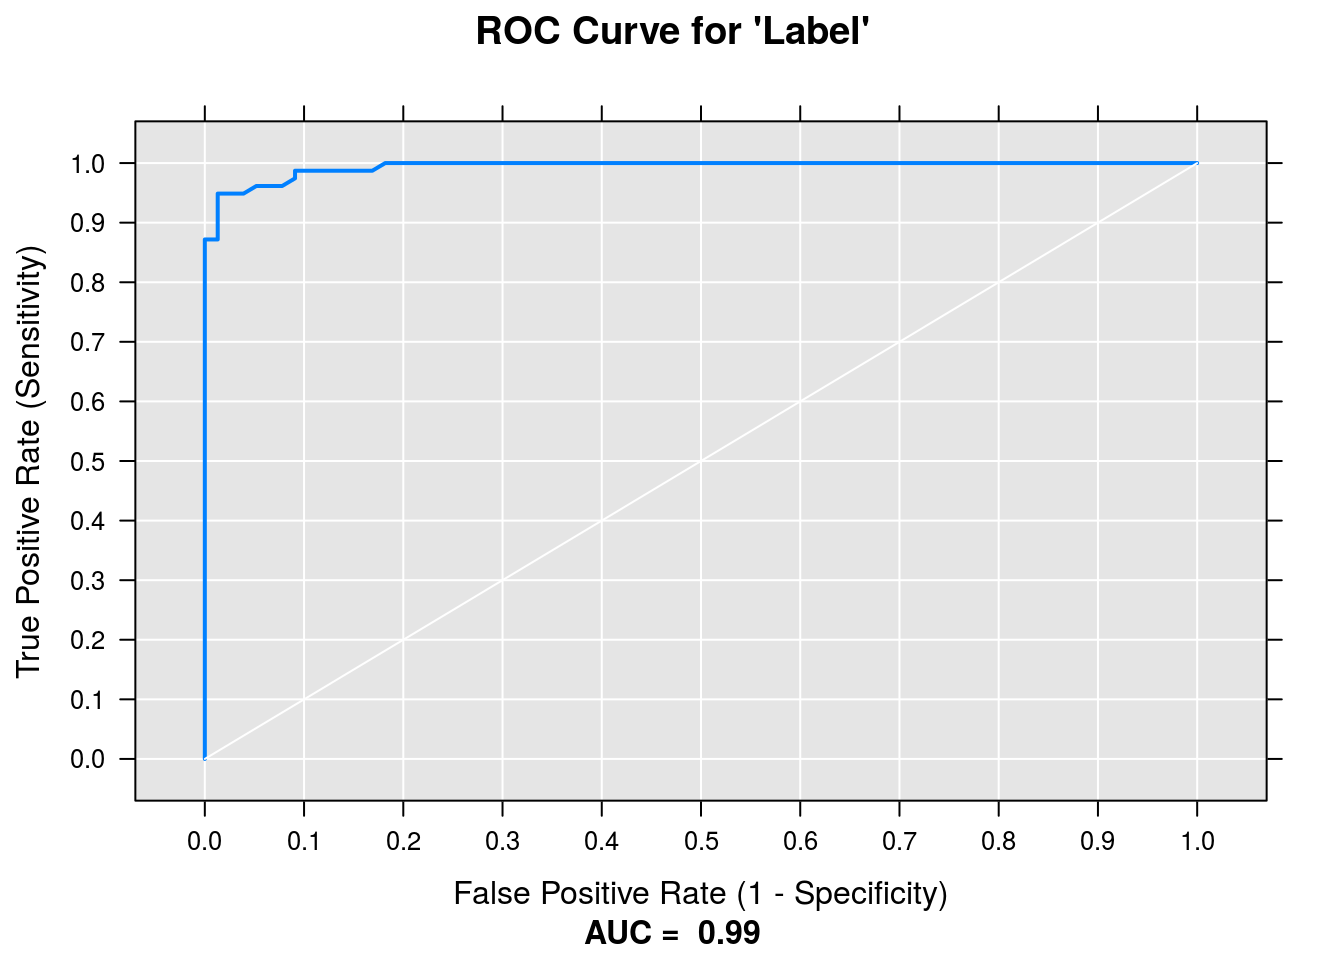
\includegraphics{mml-tutorial_files/figure-latex/featurizeTransforms-1.pdf}

\section{Retaining Features}\label{retaining-features}

While the above approach is scalable beyond datasets that can fit in
memory, it has the drawback of not being reusable. In paricular, we
can't ``pull-out'' the features we trained on our dataset for later use.

If you would like to retain the features you trained on, you can do so
by using the \texttt{featurizeImage} function in MicrosoftML directly.
It is analogous to the \texttt{mlTransforms} argumenet above.

\begin{Shaded}
\begin{Highlighting}[]
\KeywordTok{rxFeaturize}\NormalTok{(}\DataTypeTok{data =}\NormalTok{ train_df, }
            \DataTypeTok{outData =} \StringTok{"data/train.xdf"}\NormalTok{, }
            \DataTypeTok{overwrite =} \OtherTok{TRUE}\NormalTok{,}
            \DataTypeTok{mlTransforms =} \KeywordTok{list}\NormalTok{(}\KeywordTok{loadImage}\NormalTok{(}\DataTypeTok{vars =} \KeywordTok{list}\NormalTok{(}\DataTypeTok{Image =} \StringTok{"Path"}\NormalTok{)),}
                                \KeywordTok{resizeImage}\NormalTok{(}\DataTypeTok{vars =} \StringTok{"Image"}\NormalTok{, }
                                            \DataTypeTok{width =} \DecValTok{224}\NormalTok{, }\DataTypeTok{height =} \DecValTok{224}\NormalTok{, }
                                            \DataTypeTok{resizingOption =} \StringTok{"IsoPad"}\NormalTok{),}
                                \KeywordTok{extractPixels}\NormalTok{(}\DataTypeTok{vars =} \KeywordTok{list}\NormalTok{(}\DataTypeTok{Pixels =} \StringTok{"Image"}\NormalTok{)),}
                                \KeywordTok{featurizeImage}\NormalTok{(}\DataTypeTok{var =} \StringTok{"Pixels"}\NormalTok{, }
                                               \DataTypeTok{outVar =} \StringTok{"Feature"}\NormalTok{, }
                                               \DataTypeTok{dnnModel =} \StringTok{"resnet18"}\NormalTok{)),}
            \DataTypeTok{mlTransformVars =} \KeywordTok{c}\NormalTok{(}\StringTok{"Path"}\NormalTok{, }\StringTok{"Label"}\NormalTok{)) ->}\StringTok{ }\NormalTok{train_xdf}
\end{Highlighting}
\end{Shaded}

\begin{verbatim}
## Elapsed time: 00:00:22.1955525
\end{verbatim}

\begin{Shaded}
\begin{Highlighting}[]
\KeywordTok{rxFeaturize}\NormalTok{(}\DataTypeTok{data =}\NormalTok{ test_df, }\DataTypeTok{outData =} \StringTok{"data/test.xdf"}\NormalTok{, }\DataTypeTok{overwrite =} \OtherTok{TRUE}\NormalTok{,}
            \DataTypeTok{mlTransforms =} \KeywordTok{list}\NormalTok{(}\KeywordTok{loadImage}\NormalTok{(}\DataTypeTok{vars =} \KeywordTok{list}\NormalTok{(}\DataTypeTok{Image =} \StringTok{"Path"}\NormalTok{)),}
                                \KeywordTok{resizeImage}\NormalTok{(}\DataTypeTok{vars =} \StringTok{"Image"}\NormalTok{, }\DataTypeTok{width =} \DecValTok{224}\NormalTok{, }\DataTypeTok{height =} \DecValTok{224}\NormalTok{,}
                                            \DataTypeTok{resizingOption =} \StringTok{"IsoPad"}\NormalTok{),}
                                \KeywordTok{extractPixels}\NormalTok{(}\DataTypeTok{vars =} \KeywordTok{list}\NormalTok{(}\DataTypeTok{Pixels =} \StringTok{"Image"}\NormalTok{)),}
                                \KeywordTok{featurizeImage}\NormalTok{(}\DataTypeTok{var =} \StringTok{"Pixels"}\NormalTok{, }
                                               \DataTypeTok{outVar =} \StringTok{"Feature"}\NormalTok{, }
                                               \DataTypeTok{dnnModel =} \StringTok{"resnet18"}\NormalTok{)),}
            \DataTypeTok{mlTransformVars =} \KeywordTok{c}\NormalTok{(}\StringTok{"Path"}\NormalTok{, }\StringTok{"Label"}\NormalTok{)) ->}\StringTok{ }\NormalTok{test_xdf}
\end{Highlighting}
\end{Shaded}

\begin{verbatim}
## Elapsed time: 00:00:22.2479056
\end{verbatim}

\begin{Shaded}
\begin{Highlighting}[]
\NormalTok{varInfo <-}\StringTok{ }\KeywordTok{rxGetVarInfo}\NormalTok{(train_xdf)}

\NormalTok{features <-}\StringTok{ }\KeywordTok{paste}\NormalTok{(}\StringTok{"Feature"}\NormalTok{, }\DecValTok{0}\OperatorTok{:}\DecValTok{511}\NormalTok{, }\DataTypeTok{sep=}\StringTok{"."}\NormalTok{, }\DataTypeTok{collapse =} \StringTok{" + "}\NormalTok{)}
\NormalTok{form <-}\StringTok{ }\KeywordTok{as.formula}\NormalTok{(}\KeywordTok{paste}\NormalTok{(}\StringTok{"Label"}\NormalTok{, features, }\DataTypeTok{sep=}\StringTok{"~"}\NormalTok{))}
\NormalTok{model <-}\StringTok{ }\KeywordTok{rxLogisticRegression}\NormalTok{(}\DataTypeTok{formula =}\NormalTok{ form, }\DataTypeTok{data =}\NormalTok{ train_xdf)}
\end{Highlighting}
\end{Shaded}

\begin{verbatim}
## Automatically adding a MinMax normalization transform, use 'norm=Warn' or 'norm=No' to turn this behavior off.
## LBFGS multi-threading will attempt to load dataset into memory. In case of out-of-memory issues, turn off multi-threading by setting trainThreads to 1.
## Warning: Too few instances to use 32 threads, decreasing to 1 thread(s)
## Beginning optimization
## num vars: 513
## improvement criterion: Mean Improvement
## L1 regularization selected 97 of 513 weights.
## Not training a calibrator because it is not needed.
## Elapsed time: 00:00:00.6830235
## Elapsed time: 00:00:00.0022631
\end{verbatim}

\begin{Shaded}
\begin{Highlighting}[]
\KeywordTok{summary}\NormalTok{(model)}
\end{Highlighting}
\end{Shaded}

\begin{verbatim}
## Call:
## rxLogisticRegression(formula = form, data = train_xdf)
## 
## LogisticRegression (BinaryClassifierTrainer) for: Label~Feature.0+Feature.1+Feature.2+Feature.3+Feature.4+Feature.5+Feature.6+Feature.7+Feature.8+Feature.9+Feature.10+Feature.11+Feature.12+Feature.13+Feature.14+Feature.15+Feature.16+Feature.17+Feature.18+Feature.19+Feature.20+Feature.21+Feature.22+Feature.23+Feature.24+Feature.25+Feature.26+Feature.27+Feature.28+Feature.29+Feature.30+Feature.31+Feature.32+Feature.33+Feature.34+Feature.35+Feature.36+Feature.37+Feature.38+Feature.39+Feature.40+Feature.41+Feature.42+Feature.43+Feature.44+Feature.45+Feature.46+Feature.47+Feature.48+Feature.49+Feature.50+Feature.51+Feature.52+Feature.53+Feature.54+Feature.55+Feature.56+Feature.57+Feature.58+Feature.59+Feature.60+Feature.61+Feature.62+Feature.63+Feature.64+Feature.65+Feature.66+Feature.67+Feature.68+Feature.69+Feature.70+Feature.71+Feature.72+Feature.73+Feature.74+Feature.75+Feature.76+Feature.77+Feature.78+Feature.79+Feature.80+Feature.81+Feature.82+Feature.83+Feature.84+Feature.85+Feature.86+Feature.87+Feature.88+Feature.89+Feature.90+Feature.91+Feature.92+Feature.93+Feature.94+Feature.95+Feature.96+Feature.97+Feature.98+Feature.99+Feature.100+Feature.101+Feature.102+Feature.103+Feature.104+Feature.105+Feature.106+Feature.107+Feature.108+Feature.109+Feature.110+Feature.111+Feature.112+Feature.113+Feature.114+Feature.115+Feature.116+Feature.117+Feature.118+Feature.119+Feature.120+Feature.121+Feature.122+Feature.123+Feature.124+Feature.125+Feature.126+Feature.127+Feature.128+Feature.129+Feature.130+Feature.131+Feature.132+Feature.133+Feature.134+Feature.135+Feature.136+Feature.137+Feature.138+Feature.139+Feature.140+Feature.141+Feature.142+Feature.143+Feature.144+Feature.145+Feature.146+Feature.147+Feature.148+Feature.149+Feature.150+Feature.151+Feature.152+Feature.153+Feature.154+Feature.155+Feature.156+Feature.157+Feature.158+Feature.159+Feature.160+Feature.161+Feature.162+Feature.163+Feature.164+Feature.165+Feature.166+Feature.167+Feature.168+Feature.169+Feature.170+Feature.171+Feature.172+Feature.173+Feature.174+Feature.175+Feature.176+Feature.177+Feature.178+Feature.179+Feature.180+Feature.181+Feature.182+Feature.183+Feature.184+Feature.185+Feature.186+Feature.187+Feature.188+Feature.189+Feature.190+Feature.191+Feature.192+Feature.193+Feature.194+Feature.195+Feature.196+Feature.197+Feature.198+Feature.199+Feature.200+Feature.201+Feature.202+Feature.203+Feature.204+Feature.205+Feature.206+Feature.207+Feature.208+Feature.209+Feature.210+Feature.211+Feature.212+Feature.213+Feature.214+Feature.215+Feature.216+Feature.217+Feature.218+Feature.219+Feature.220+Feature.221+Feature.222+Feature.223+Feature.224+Feature.225+Feature.226+Feature.227+Feature.228+Feature.229+Feature.230+Feature.231+Feature.232+Feature.233+Feature.234+Feature.235+Feature.236+Feature.237+Feature.238+Feature.239+Feature.240+Feature.241+Feature.242+Feature.243+Feature.244+Feature.245+Feature.246+Feature.247+Feature.248+Feature.249+Feature.250+Feature.251+Feature.252+Feature.253+Feature.254+Feature.255+Feature.256+Feature.257+Feature.258+Feature.259+Feature.260+Feature.261+Feature.262+Feature.263+Feature.264+Feature.265+Feature.266+Feature.267+Feature.268+Feature.269+Feature.270+Feature.271+Feature.272+Feature.273+Feature.274+Feature.275+Feature.276+Feature.277+Feature.278+Feature.279+Feature.280+Feature.281+Feature.282+Feature.283+Feature.284+Feature.285+Feature.286+Feature.287+Feature.288+Feature.289+Feature.290+Feature.291+Feature.292+Feature.293+Feature.294+Feature.295+Feature.296+Feature.297+Feature.298+Feature.299+Feature.300+Feature.301+Feature.302+Feature.303+Feature.304+Feature.305+Feature.306+Feature.307+Feature.308+Feature.309+Feature.310+Feature.311+Feature.312+Feature.313+Feature.314+Feature.315+Feature.316+Feature.317+Feature.318+Feature.319+Feature.320+Feature.321+Feature.322+Feature.323+Feature.324+Feature.325+Feature.326+Feature.327+Feature.328+Feature.329+Feature.330+Feature.331+Feature.332+Feature.333+Feature.334+Feature.335+Feature.336+Feature.337+Feature.338+Feature.339+Feature.340+Feature.341+Feature.342+Feature.343+Feature.344+Feature.345+Feature.346+Feature.347+Feature.348+Feature.349+Feature.350+Feature.351+Feature.352+Feature.353+Feature.354+Feature.355+Feature.356+Feature.357+Feature.358+Feature.359+Feature.360+Feature.361+Feature.362+Feature.363+Feature.364+Feature.365+Feature.366+Feature.367+Feature.368+Feature.369+Feature.370+Feature.371+Feature.372+Feature.373+Feature.374+Feature.375+Feature.376+Feature.377+Feature.378+Feature.379+Feature.380+Feature.381+Feature.382+Feature.383+Feature.384+Feature.385+Feature.386+Feature.387+Feature.388+Feature.389+Feature.390+Feature.391+Feature.392+Feature.393+Feature.394+Feature.395+Feature.396+Feature.397+Feature.398+Feature.399+Feature.400+Feature.401+Feature.402+Feature.403+Feature.404+Feature.405+Feature.406+Feature.407+Feature.408+Feature.409+Feature.410+Feature.411+Feature.412+Feature.413+Feature.414+Feature.415+Feature.416+Feature.417+Feature.418+Feature.419+Feature.420+Feature.421+Feature.422+Feature.423+Feature.424+Feature.425+Feature.426+Feature.427+Feature.428+Feature.429+Feature.430+Feature.431+Feature.432+Feature.433+Feature.434+Feature.435+Feature.436+Feature.437+Feature.438+Feature.439+Feature.440+Feature.441+Feature.442+Feature.443+Feature.444+Feature.445+Feature.446+Feature.447+Feature.448+Feature.449+Feature.450+Feature.451+Feature.452+Feature.453+Feature.454+Feature.455+Feature.456+Feature.457+Feature.458+Feature.459+Feature.460+Feature.461+Feature.462+Feature.463+Feature.464+Feature.465+Feature.466+Feature.467+Feature.468+Feature.469+Feature.470+Feature.471+Feature.472+Feature.473+Feature.474+Feature.475+Feature.476+Feature.477+Feature.478+Feature.479+Feature.480+Feature.481+Feature.482+Feature.483+Feature.484+Feature.485+Feature.486+Feature.487+Feature.488+Feature.489+Feature.490+Feature.491+Feature.492+Feature.493+Feature.494+Feature.495+Feature.496+Feature.497+Feature.498+Feature.499+Feature.500+Feature.501+Feature.502+Feature.503+Feature.504+Feature.505+Feature.506+Feature.507+Feature.508+Feature.509+Feature.510+Feature.511
## Data: train_xdf (RxXdfData Data Source)
## File name: data/train.xdf 
## 
## 
## First 20 of 97 Non-zero Coefficients:
## (Bias): 0.2091156
## Feature.487: -1.327465
## Feature.431: 0.9092103
## Feature.460: -0.8586729
## Feature.157: 0.7992205
## Feature.47: -0.7986112
## Feature.511: -0.6897881
## Feature.315: -0.6197985
## Feature.270: 0.6049663
## Feature.233: -0.5948368
## Feature.62: 0.5754997
## Feature.456: 0.56534
## Feature.293: 0.5637971
## Feature.269: -0.5151423
## Feature.441: -0.493934
## Feature.88: 0.483808
## Feature.406: -0.4684003
## Feature.93: 0.465048
## Feature.145: -0.4564239
## Feature.224: -0.4489715
\end{verbatim}

\begin{Shaded}
\begin{Highlighting}[]
\NormalTok{score <-}\KeywordTok{rxPredict}\NormalTok{(model, test_xdf, }\DataTypeTok{extraVarsToWrite =} \StringTok{"Label"}\NormalTok{)}
\end{Highlighting}
\end{Shaded}

\begin{verbatim}
## Elapsed time: 00:00:00.1706593
\end{verbatim}

\begin{Shaded}
\begin{Highlighting}[]
\KeywordTok{sum}\NormalTok{(score}\OperatorTok{$}\NormalTok{Label}\OperatorTok{==}\NormalTok{score}\OperatorTok{$}\NormalTok{PredictedLabel)}\OperatorTok{/}\KeywordTok{nrow}\NormalTok{(score)}
\end{Highlighting}
\end{Shaded}

\begin{verbatim}
## [1] 0.9870968
\end{verbatim}

\begin{Shaded}
\begin{Highlighting}[]
\KeywordTok{rxRocCurve}\NormalTok{(}\StringTok{"Label"}\NormalTok{,}\StringTok{"Probability"}\NormalTok{,score)}
\end{Highlighting}
\end{Shaded}

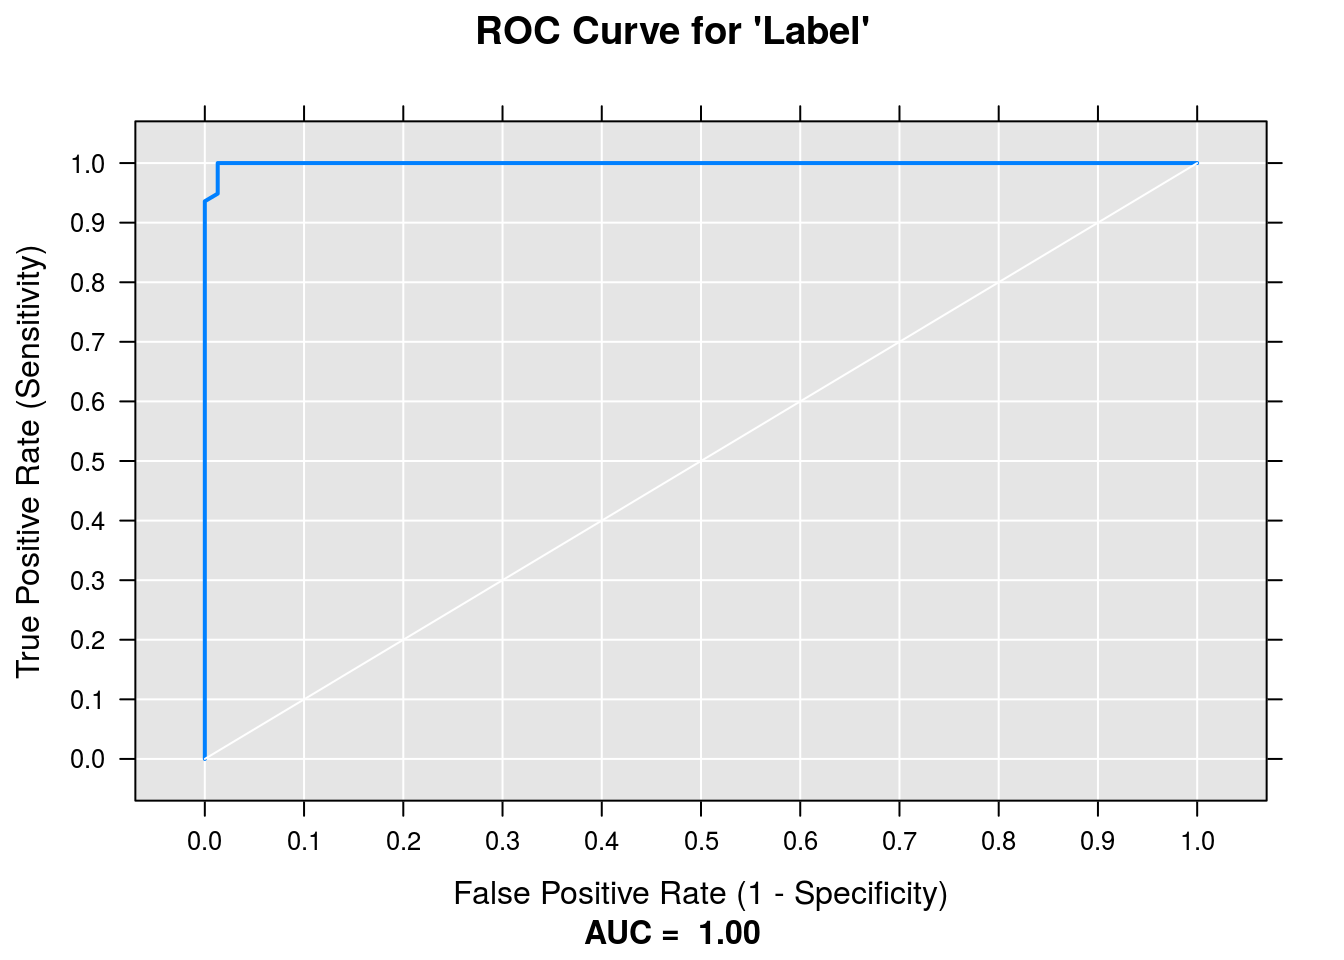
\includegraphics{mml-tutorial_files/figure-latex/featurizeImage-1.pdf}

\bibliography{book.bib}


\end{document}
